\documentclass[aspectratio=43]{beamer}
\usepackage[space,hyperref,UTF8]{ctex}
\usepackage{graphicx}
\usepackage{amsmath}
\usepackage{amssymb}
\usepackage{booktabs}%表格
\graphicspath{{图片/}}%可以不用写路径
\setbeamertemplate{navigation symbols}{}%不出现导航栏
\setbeamerfont{toc}{size=\small}
\usepackage{multicol}%双栏排版
\usepackage{subfigure}%插入子图
\usefonttheme[onlymath]{serif}%数学公式无衬线字体
\usepackage{color}%字体背景颜色
\usepackage{framed}
\definecolor{shadecolor}{RGB}{242, 242, 255}
\usetheme{Madrid}
\usecolortheme{rose}







%\useoutertheme{smoothbars}
%\useoutertheme{smoothbars}:
%infolines,miniframes,sidebar,split,shadow,tree,smoothtree
\mode<presentation>
\title{基于机器视觉的物品抓取视觉标定方法设计}
%\subtitle{毕业设计}
\author{王云龙}
\institute{机电工程学院}
\date{\today}
%显示二级标题
\AtBeginSubsection[]
{
	\begin{frame}[shrink]
		\frametitle{Table of Contents}
		\tableofcontents[currentsubsection]
	\end{frame}
}

\begin{document}
	%标题页

	\begin{frame}
		\titlepage
		\begin{figure}[htbp]
			\begin{center}
				
\includegraphics[scale=0.1]{logo2.jpg}
			\end{center}
		\end{figure}
	\end{frame}

	%目录页
	\begin{frame}[shrink]%3:使其字体缩小,同样使用其它页
		%1:[allowframebreaks]%一页不够,显示两页
		\frametitle{Table of Contents}
%		\begin{multicols}{2}%2:目录分栏显示
			\tableofcontents
%		\end{multicols}
	\end{frame}
	
\section{任务概览}

\begin{frame}
	\frametitle{任务思路}

\end{frame}






\begin{frame}
	\frametitle{什么是相机标定}
	拍照$\longrightarrow$二维图像1$\xrightarrow{\text{图像处理}}$二维图像2$\xrightarrow{{\color[RGB]{240, 0, 0} \text{相机标定}}}$实际意义数据
	\begin{itemize}
		\item 外参矩阵:摄像机在三维世界的坐标关系
		\item 内参矩阵:相机内部的几何和光学特性
		\item 畸变系数:像素点没有落在理论位置上,产生了偏移和变形
		\item ${\color{blue} \text{结构参数:左右相机的位置关系}}$
	\end{itemize}
\end{frame}

\begin{frame}
	\frametitle{相机标定方法分类}
	\begin{figure}
	\begin{center}
		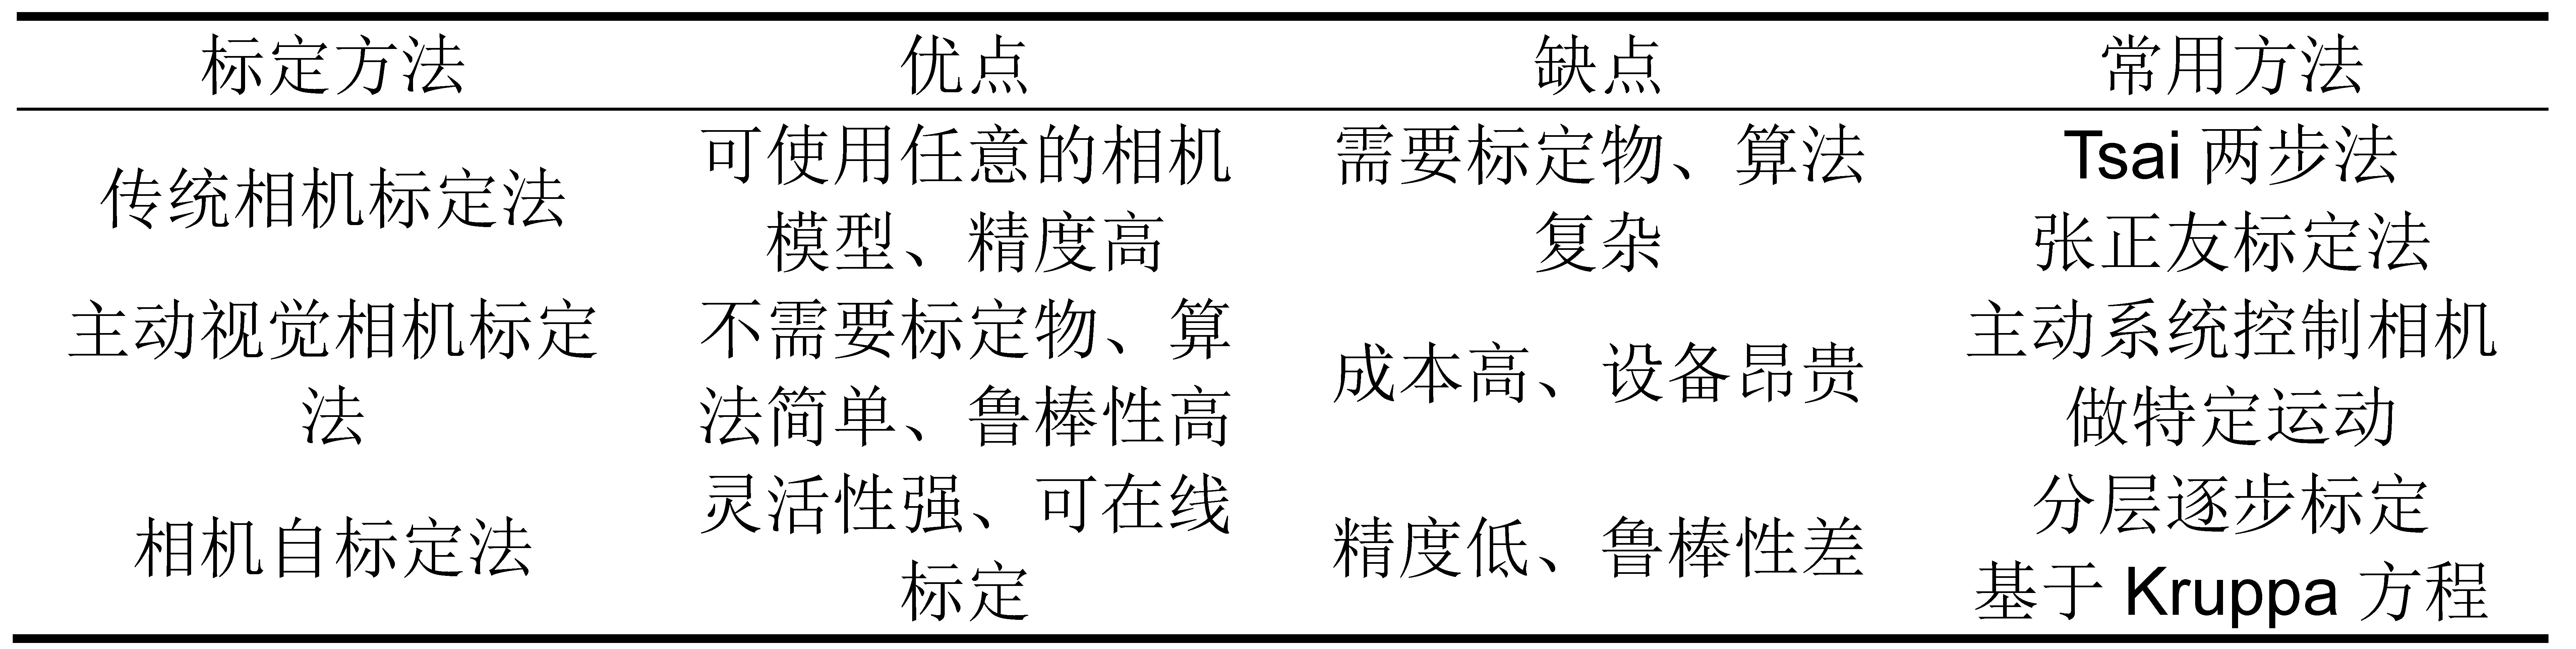
\includegraphics[scale=0.765]{相机标定方法}
	\end{center}
	\end{figure}
\end{frame}

	
\section{工具选择}

\subsection{硬件选择}

\begin{frame}
	\frametitle{硬件选择}
	\begin{itemize}
		\item 摄像头
		\item 标定板
		\item 电脑
	\end{itemize}
\end{frame}

\begin{frame}
	\frametitle{摄像头比较及选择}	
	\begin{itemize}
		\item 单目摄像头
		\item 双目摄像头
		\item 鱼眼摄像头
		\item 深度摄像头	
	\end{itemize}	
\end{frame}	

\begin{frame}
	\frametitle{单目摄像头}	
\end{frame}	

\begin{frame}
	\frametitle{双目摄像头}	
\end{frame}	

\begin{frame}
	\frametitle{鱼眼摄像头}	
\end{frame}	

\begin{frame}
	\frametitle{深度摄像头}	
\end{frame}	

\begin{frame}
	\frametitle{标定板}
	\begin{columns}
	\column{5cm}
	\begin{figure}\label{标定板}
	\begin{center}
		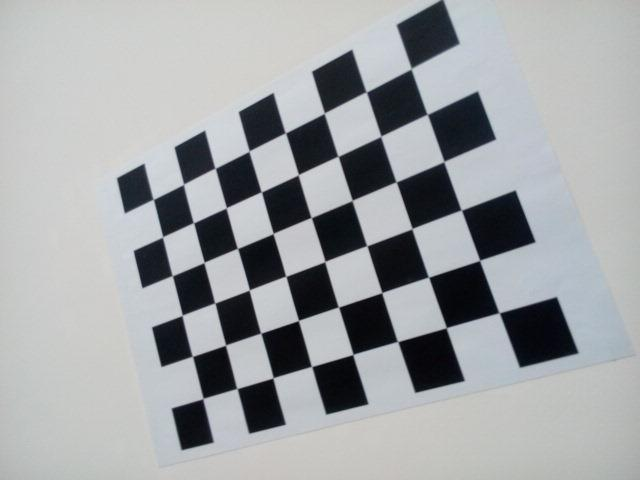
\includegraphics[scale=0.25]{标定板}
		\caption{方格标定板}
	\end{center}
	\end{figure}
	\column{5cm}
	\begin{itemize}
		\item 黑白方块间隔组成的二维平面
		\item 更简单,容易处理
		\item 二维图像相比三维物体会缺少部分信息
		\item 不同方位,多次拍摄
	\end{itemize}	
	\end{columns}
		
\end{frame}	






\subsection{软件选择}


\begin{frame}
	\frametitle{软件选择}
	\begin{itemize}
		\item 图像处理软件
		\begin{itemize}
			\item Halcon
			\item OpenCV
			\item VisionPro
		\end{itemize}
		\item 上位机软件(可选)
	\end{itemize}
\end{frame}

\begin{frame}
	\frametitle{Halcon}	
\end{frame}	

\begin{frame}
	\frametitle{OpenCV}	
\end{frame}

\begin{frame}
	\frametitle{VisionPro}	
\end{frame}		


\begin{frame}
	\frametitle{编程语言选择}
	\begin{itemize}
		\item Python
		\item C++
		\item C\#
		\item Matlab
	\end{itemize}
\end{frame}




\begin{frame}
	\frametitle{最终选择}
	\begin{itemize}
		\item 双目摄像头
		\item 标定板
		\item 编程语言:C++
		\item 图像处理:OpenCV
		\item 上位机软件:Github获取
	\end{itemize}
\end{frame}			


\section{研究内容}



%	\begin{frame}
	%	\frametitle{棱镜模型}
	%	\begin{center}
		%		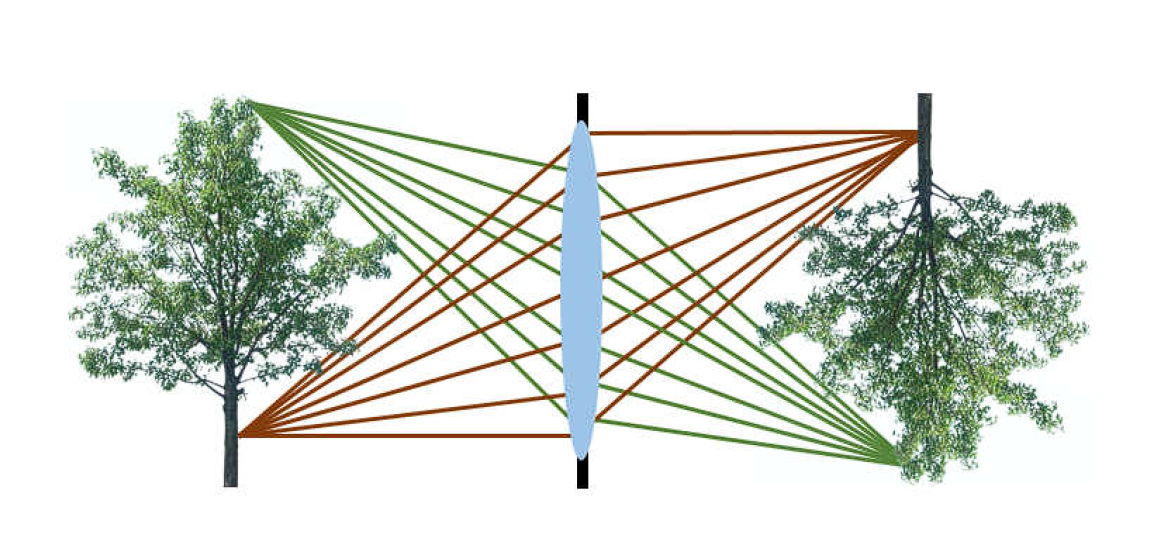
\includegraphics[scale=0.3]{棱镜模型}
		%	\end{center}	
	%	\end{frame}	
\subsection{相机模型}
\begin{frame}
	\frametitle{小孔成像模型}
	%	一个问题:棱镜模型可以汇聚所有的光线,但是小孔成像只能将其汇聚到孔内,其它的光线怎么办?
	\begin{center}
		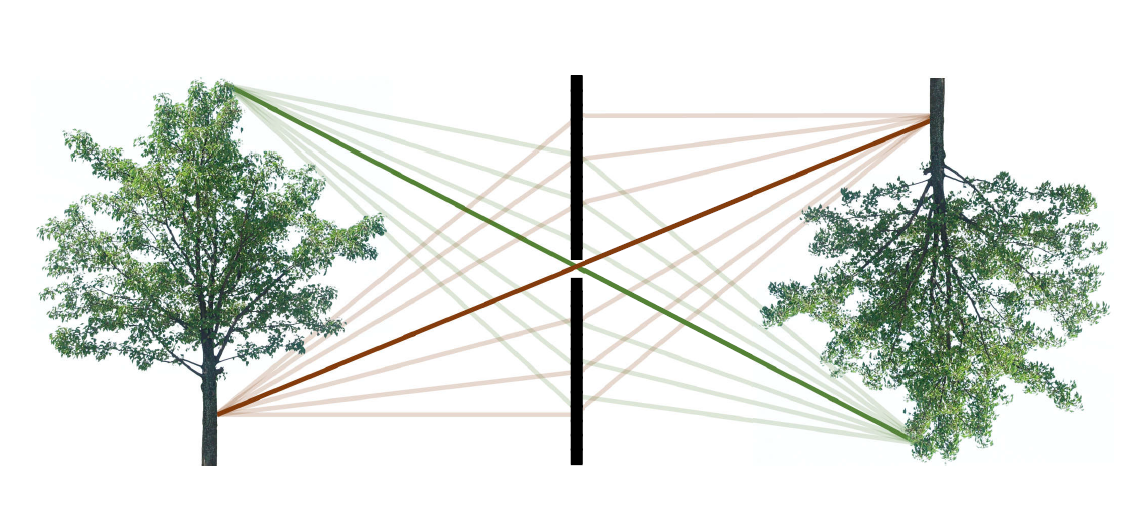
\includegraphics[scale=0.3]{小孔成像模型1}
	\end{center}
	\begin{center}
		\begin{itemize}
			\item 简单没有镜头
			\item 有一个小的光圈
			\item 真实世界的物体发出光线通过光圈
		\end{itemize}
	\end{center}
	
\end{frame}

\begin{frame}
	\frametitle{小孔成像模型简化}
	\begin{figure}
		\begin{center}
			\subfigure[实际物体投影]
			{
				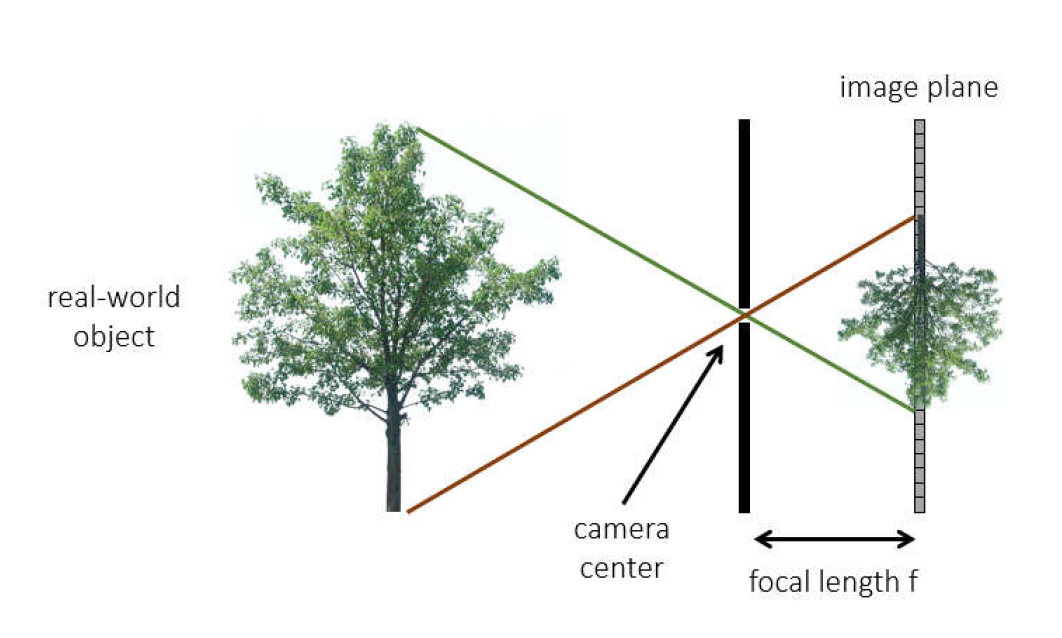
\includegraphics[scale=0.22]{小孔成像模型2}
			}
			\subfigure[简化示意图]
			{
				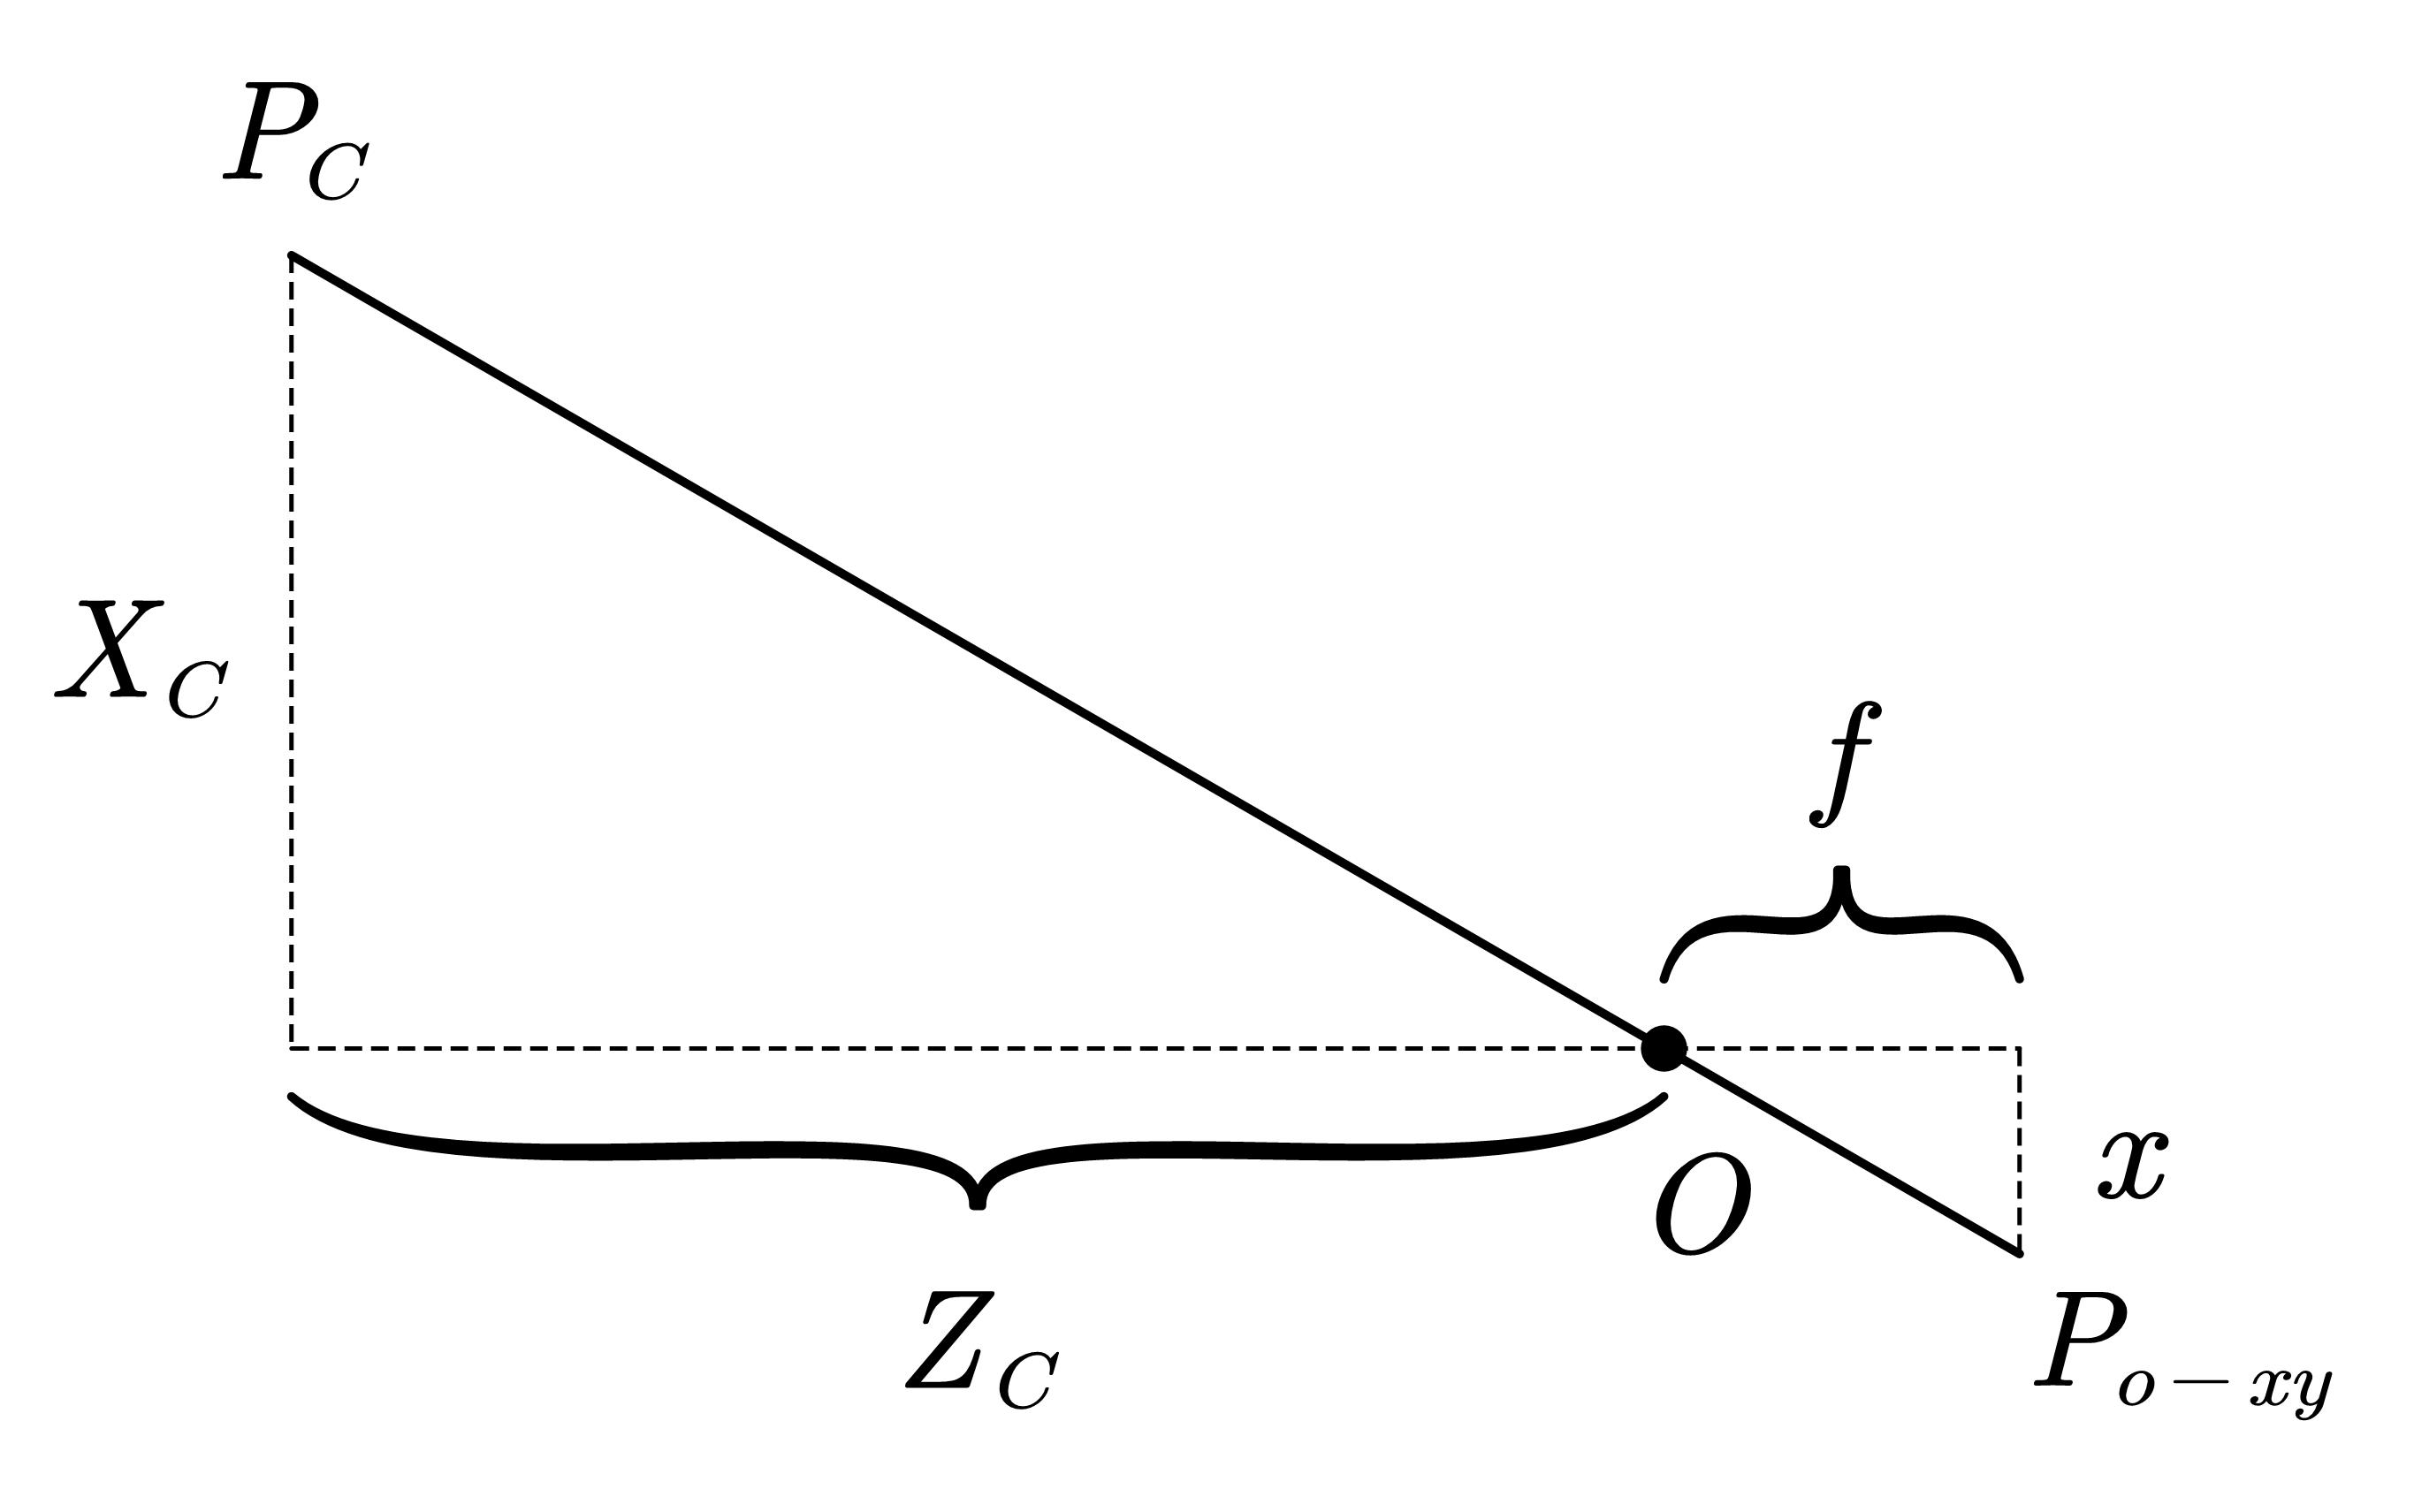
\includegraphics[scale=0.55]{小孔成像模型原理1}
			}
		\end{center}	
	\end{figure}
	
	\begin{gather}
		\left\{ \begin{array}{c}
			x=-f\cdot \frac{X_c}{Z_c}\\
			\\
			y=-f\cdot \frac{Y_c}{Z_c}\\
		\end{array} \right. 	
	\end{gather}
\end{frame}

\begin{frame}
	\frametitle{小孔成像模型的改进}
	\begin{figure}
		\setcounter{subfigure}{0}
		\begin{center}
			\subfigure[实际物体投影]
			{
				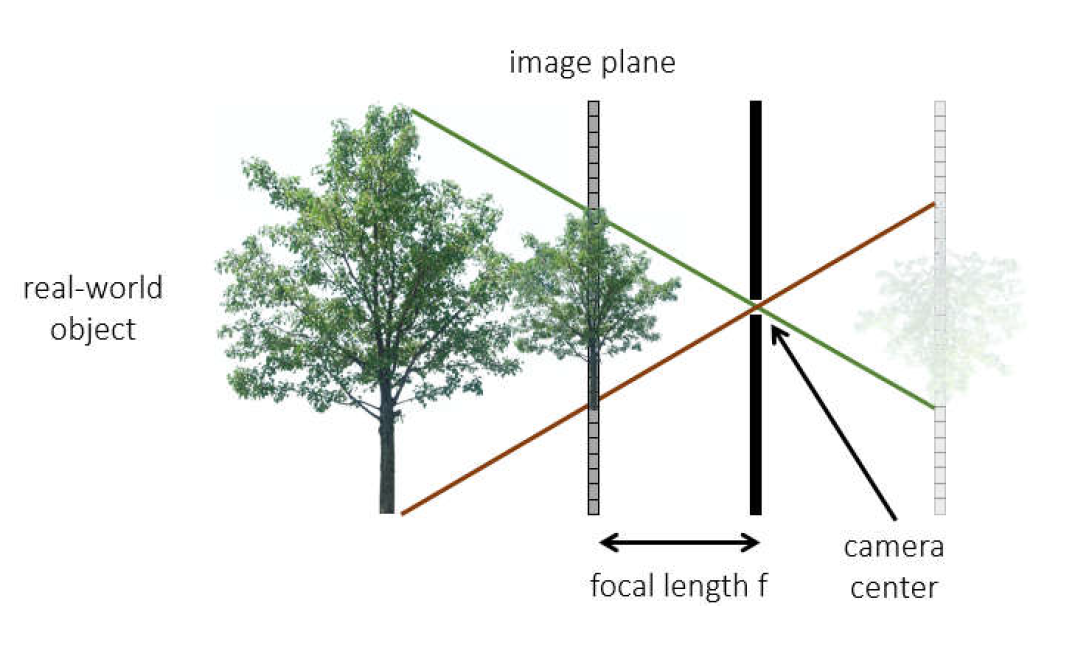
\includegraphics[scale=0.22]{小孔成像模型3}
			}
			\subfigure[简化示意图]
			{
				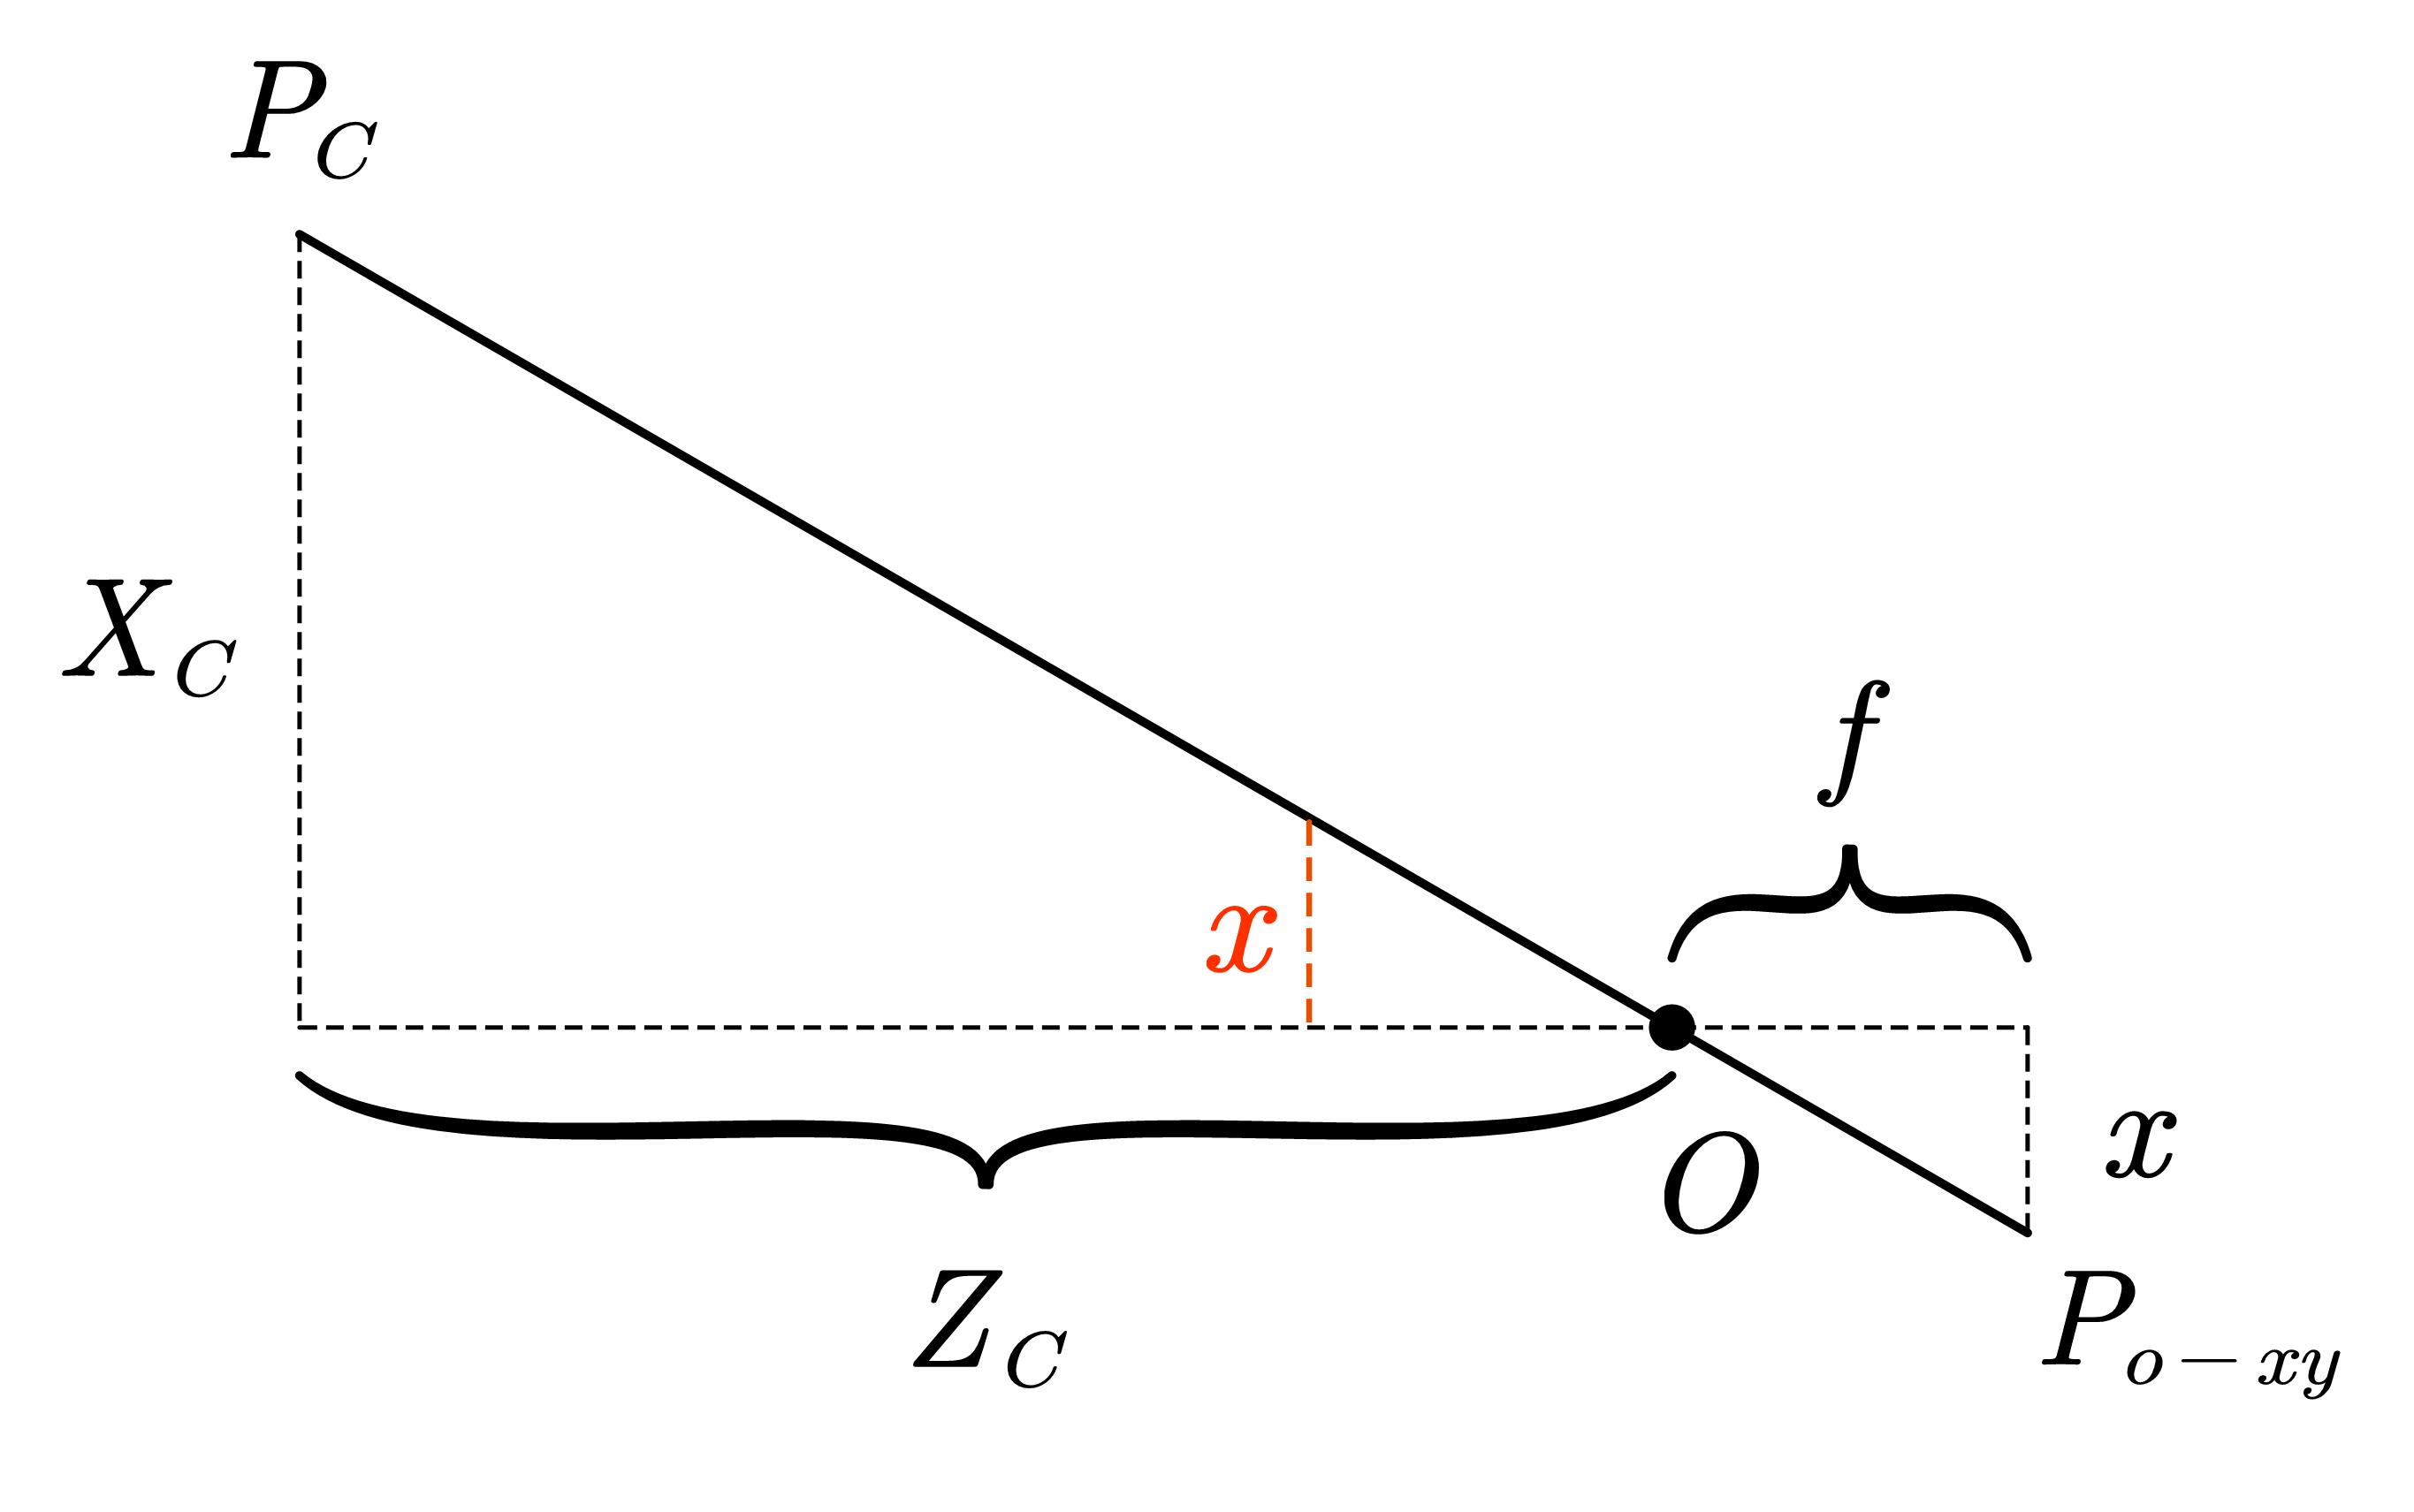
\includegraphics[scale=0.55]{小孔成像模型原理2}
			}		
		\end{center}
	\end{figure}
	\begin{gather}
		\left\{ \begin{array}{c}
			x=f\cdot \frac{X_c}{Z_c}\\
			\\
			y=f\cdot \frac{Y_c}{Z_c}\\
		\end{array} \right. 	
	\end{gather}
\end{frame}

\subsection{相机畸变}

\begin{frame}
	\frametitle{什么是畸变?}
	
	为了获得好的成像效果,我们在相机的前方加了透镜。
	透镜的加入对成像过程中光线的传播会产生新的影响: 
	\begin{itemize}
		\item 透镜自身的形状对光线传播的影响
		\item 透镜和成像平面不能完全平行,物体投影的位置发生变化
	\end{itemize}
\end{frame}

\begin{frame}
	\frametitle{畸变分类}
	\begin{itemize}
		\item 径向畸变:透镜形状
		\begin{itemize}
			\item 桶型畸变:离光轴距离越远,图像放大率越小
			\item 枕型畸变:离光轴距离越远,图像放大率越小
		\end{itemize}
		\item 切向畸变:透镜与成像平面不平行
	\end{itemize}
\end{frame}

\begin{frame}
	\frametitle{径向畸变}
	\begin{center}
		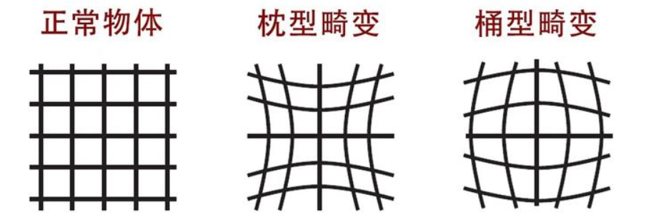
\includegraphics[scale = 0.35]{畸变失真.png}
	\end{center}
	\vspace{-0.6em}
	\begin{gather}
		x_{corrected}=x\left( 1+k_1r^2+k_2r^4+k_3r^6 \right) 
		\\
		y_{corrected}=y\left( 1+k_1r^2+k_2r^4+k_3r^6 \right) 	
	\end{gather}
	
	
	\begin{itemize}
		\item $(x,y)$是没有畸变的像素点
		\item $(x_{corrected},y_{corrected})$是畸变后的位置
		\item 参数:${\color{red} k_1},{\color{red} k_2},{\color{blue} k_3}$\footnote{一般使用前两项,鱼眼相机使用第三项}
	\end{itemize}
\end{frame}

\begin{frame}
	\frametitle{切向畸变}
	\begin{center}
		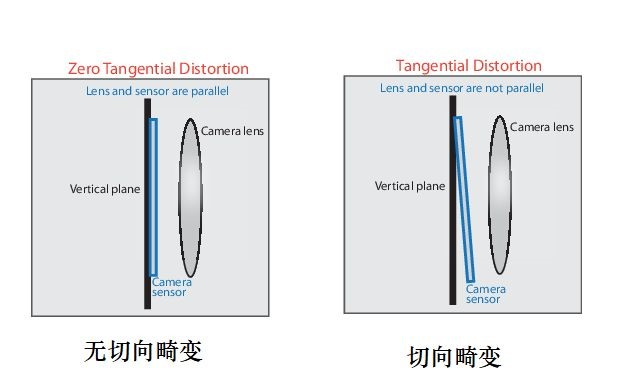
\includegraphics[scale=0.35]{切向畸变.jpg}
	\end{center}
	\vspace{-0.6em}
	\begin{gather}
		x_{corrected}=x+2p_1xy+p_2\left( r^2+2x^2 \right) 
		\\
		y_{corrected}=y+p_1\left( r^2+2y^2 \right) +2p_2xy
	\end{gather}
	\begin{center}
		参数:${\color[RGB]{240, 0, 0} p_1,p_2}$
	\end{center}
\end{frame}

\begin{frame}
	\frametitle{畸变合并}
	\begin{gather}
		x_{corrected}=x\left( 1+k_1r^2+k_2r^4+k_3r^6 \right) +{\color[RGB]{128, 0, 255} \left[ 2p_1xy+p_2\left( r^2+2x^2 \right) \right] }
		\\
		y_{corrected}=y\left( 1+k_1r^2+k_2r^4+k_3r^6 \right) +{\color[RGB]{128, 0, 255} \left[ 2p_2xy+p_1\left( r^2+2y^2 \right) \right] }	
	\end{gather}
\end{frame}


		
	\subsection{数理基础:矩阵、坐标系、齐次坐标}
		
\begin{frame}	
	\frametitle{坐标系}
	\begin{itemize}
		\item 世界坐标系:$O_{W} -X_{W} Y_{W} Z_{W} $
		\item 相机坐标系:$O_{C} -X_{C} Y_{C} Z_{C} $
		\item 图像坐标系:$o-xy$
		\item 像素坐标系:$o-uv $
	\end{itemize}
\end{frame}

\begin{frame}
\frametitle{世界坐标系(3D)}
\begin{itemize}
	\item 描述相机在真实三维世界的坐标
	\item 坐标系用$O_{W} -X_{W} Y_{W} Z_{W} $表示,单位$m$
	\item 双目视觉中一般将世界坐标系原点定在左相机或者右相机或者二者$X$轴方向的中点
\end{itemize}
\end{frame}

\begin{frame}
		\frametitle{相机坐标系(3D)}
\begin{itemize}
	\item 以相机光学中心为原点,$Z$轴与相机光轴重合
	\item 坐标系用$O_{C} -X_{C} Y_{C} Z_{C} $表示,单位$m$
\end{itemize}
\end{frame}

\begin{frame}
		\frametitle{图像坐标系(2D)}
\begin{itemize}
	\item 二维图像的中心点为原点
	\item 坐标系用$o-xy$表示,单位$mm$
\end{itemize}		
\end{frame}

\begin{frame}
\frametitle{像素坐标系(2D)}
\begin{itemize}
	\item 图像的基本单位是像素($pixel$)
	\item 图像的像素值以矩阵形式保存
	\item 坐标原点在图像左上角,坐标系用$o-uv $表示,单位为像素($pixel$)
\end{itemize}
\end{frame}

\begin{frame}
	\frametitle{矩阵}
	\begin{itemize}
		\item 内参矩阵$M_1$:相机坐标(3D)如何变换到像素坐标(2D)
		\item 外参矩阵$M_2$:世界坐标(3D)如何变换到相机坐标(3D)
		\begin{itemize}
			\item 平移矩阵:$T$
			\item 旋转矩阵:$R=R_X\cdot R_Y\cdot R_Z$
			\begin{itemize}
				\item 绕Z轴旋转:$R_Z$
				\item 绕X轴旋转:$R_X$
				\item 绕Y轴旋转:$R_Y$
			\end{itemize}
		\end{itemize}
		\item 单应性矩阵$H$:世界坐标系与像素坐标系之间的映射关系
		\item 本征矩阵
		\item 基本矩阵
	\end{itemize}
\end{frame}

\begin{frame}
	\frametitle{旋转矩阵:绕Z轴旋转}
	\begin{columns}
		\column{5cm}
		\begin{figure}
			\begin{center}
				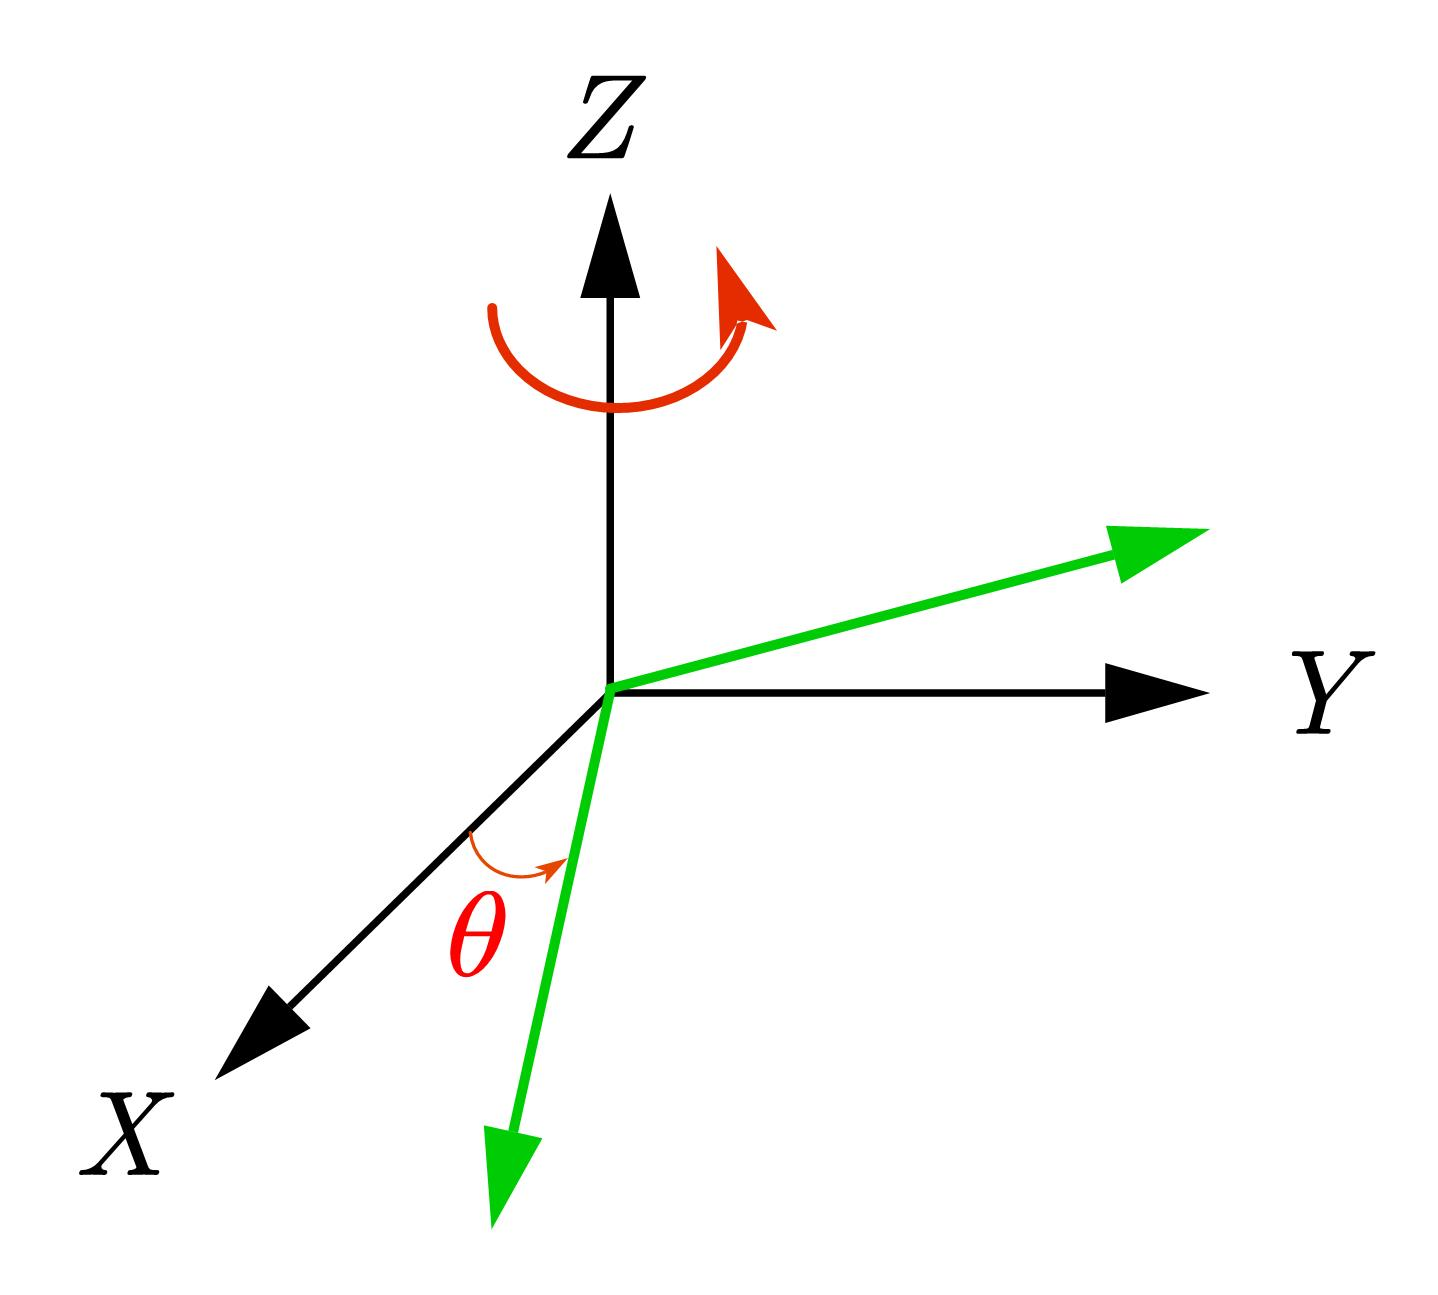
\includegraphics[scale=1]{旋转矩阵Z}
			\end{center}
		\end{figure}
		\column{6cm}
		\begin{gather}
			R_Z\left( \theta \right) =\left[ \begin{matrix}
				\cos \theta&		-\sin \theta&		0\\
				\sin \theta&		\cos \theta&		0\\
				0&		0&		1\\
			\end{matrix} \right] 	
		\end{gather}	
	\end{columns}
\end{frame}

\begin{frame}
	\frametitle{旋转矩阵:绕X轴旋转}
	\begin{columns}
		\column{5cm}
		\begin{figure}
			\begin{center}
				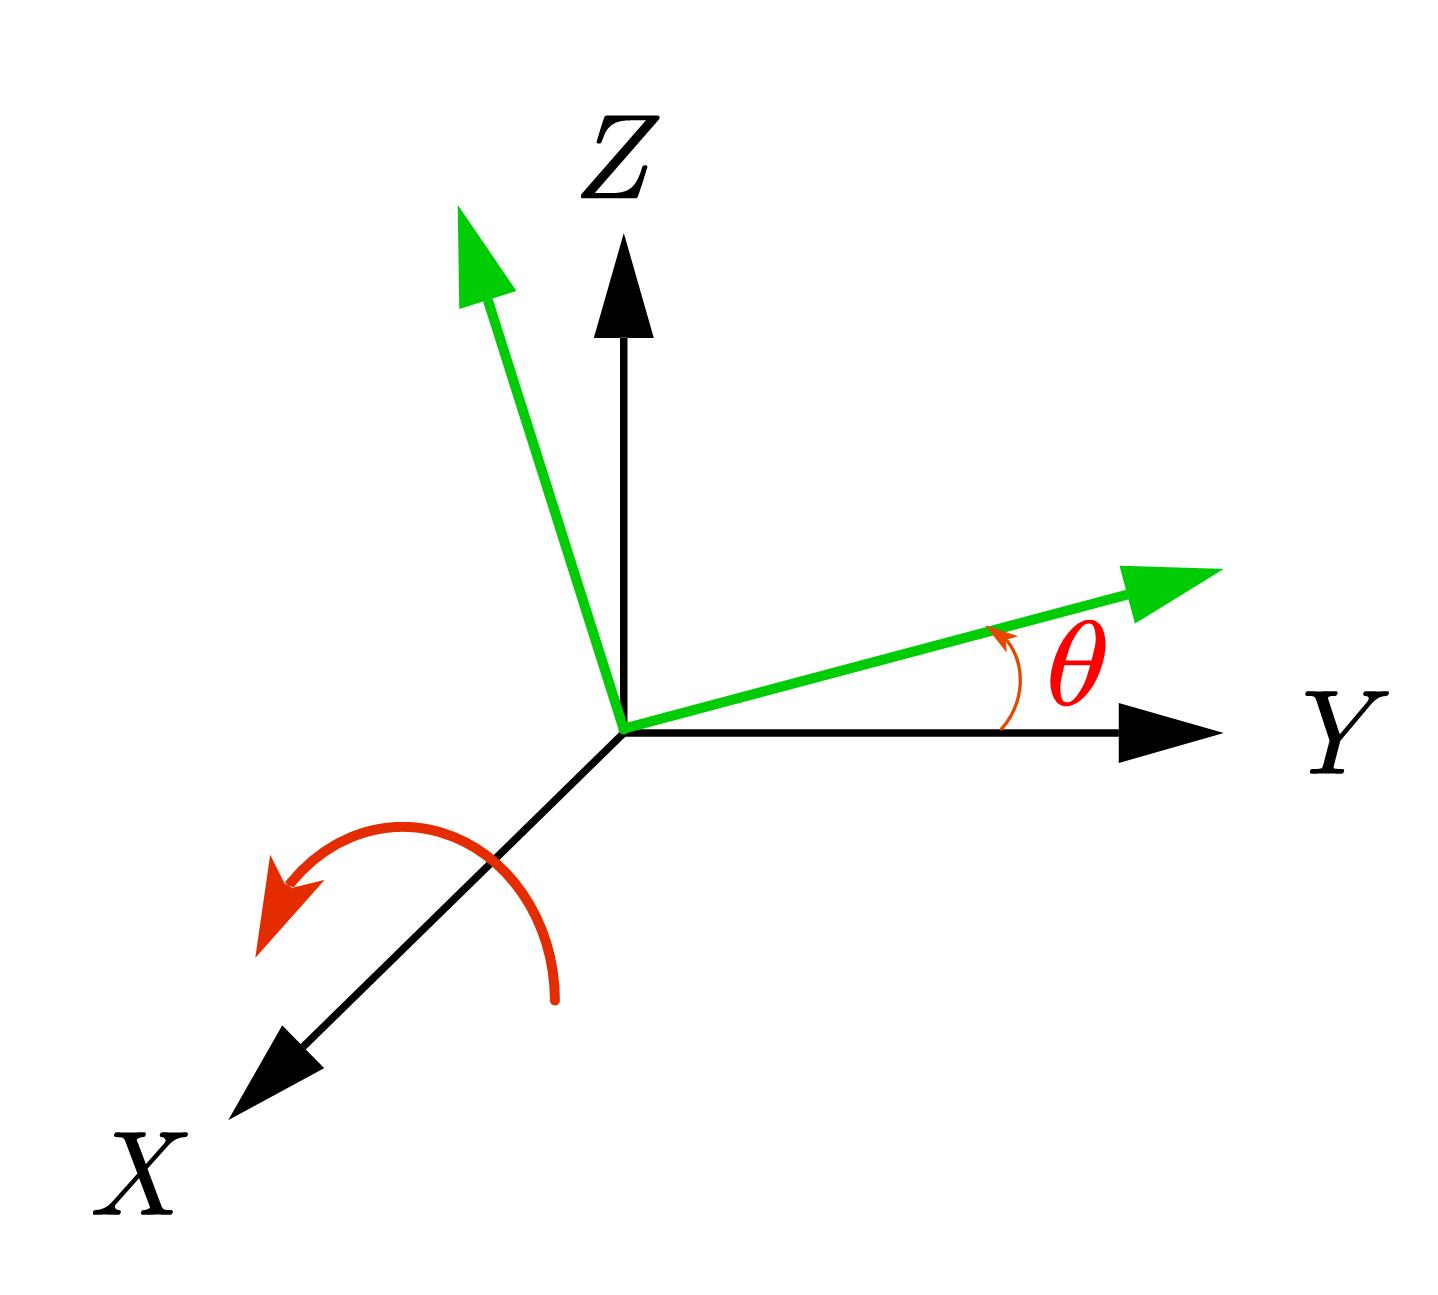
\includegraphics[scale=1]{旋转矩阵X}
			\end{center}
		\end{figure}
		\column{6cm}
		\begin{gather}
			R_X\left( \theta \right) =\left[ \begin{matrix}
				1&		0&		0\\
				0&		\cos \theta&		-\sin \theta\\
				0&		\sin \theta&		\cos \theta\\
			\end{matrix} \right] 	
		\end{gather}		
	\end{columns}
\end{frame}

\begin{frame}
	\frametitle{旋转矩阵:绕Y轴旋转}
	\begin{columns}
		\column{5cm}
		\begin{figure}
			\begin{center}
				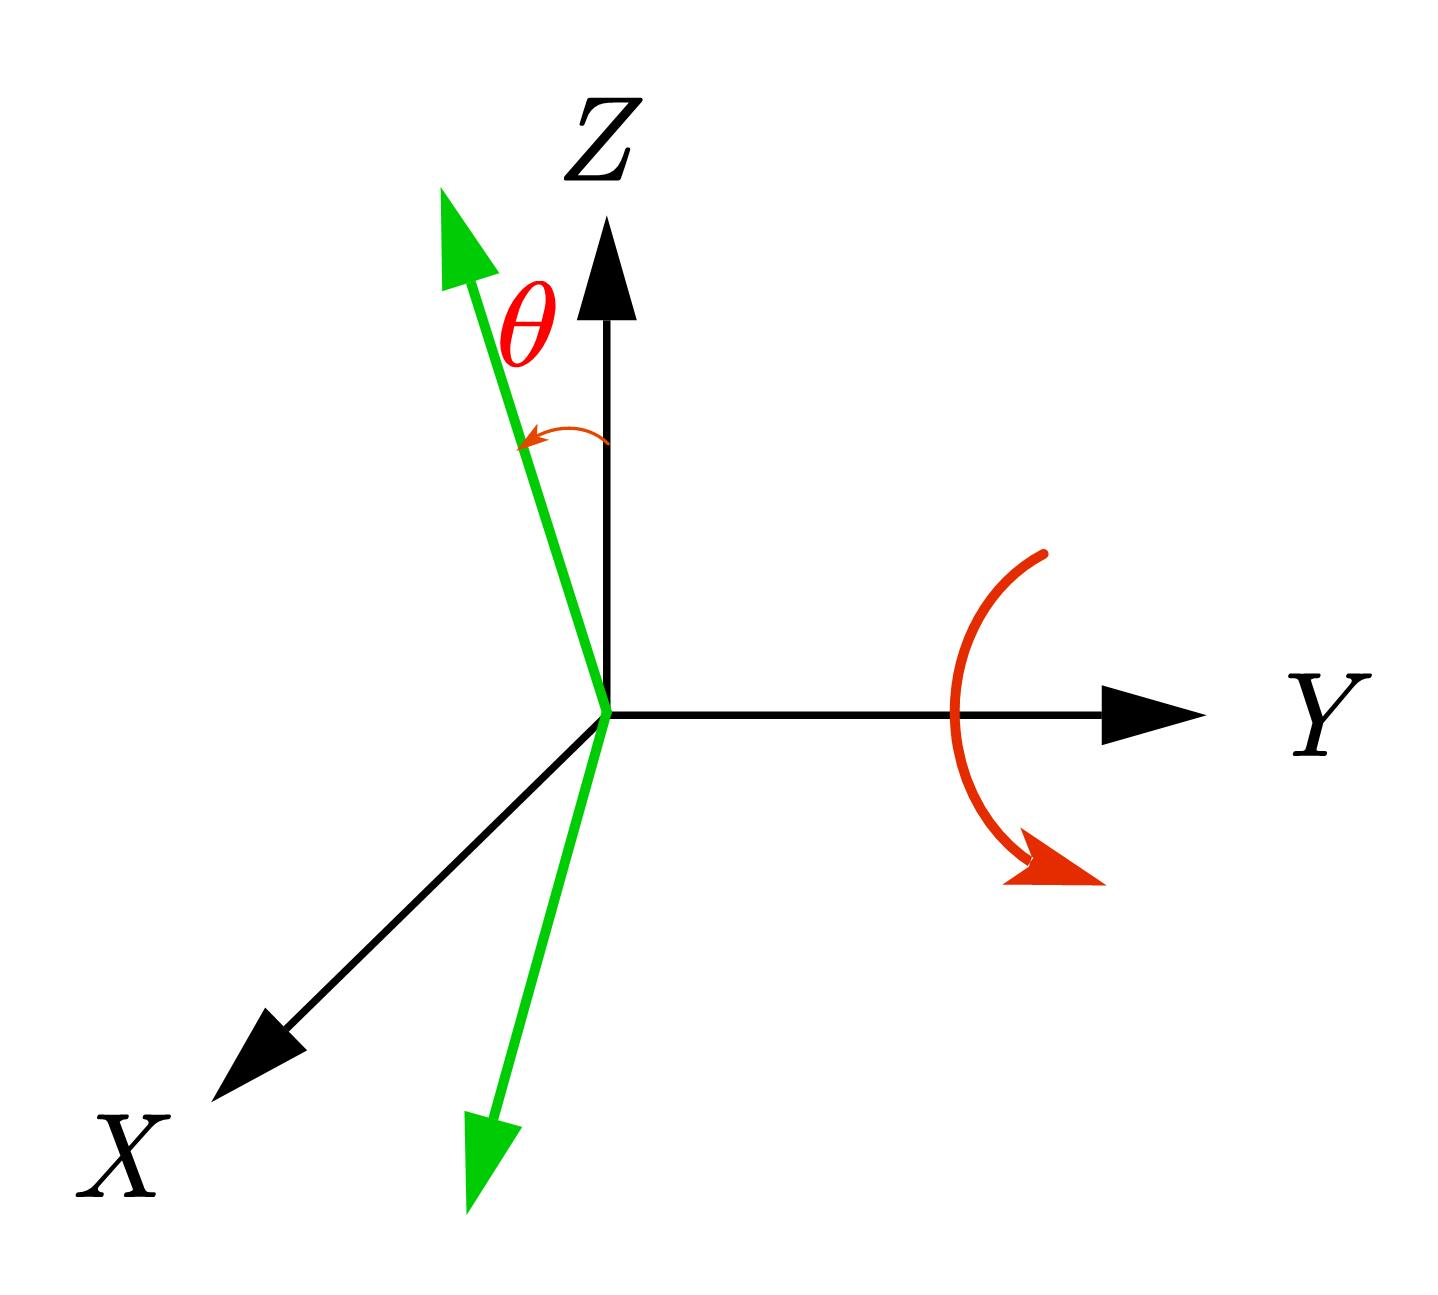
\includegraphics[scale=1]{旋转矩阵Y}
			\end{center}
		\end{figure}
		\column{6cm}
		\begin{gather}
			R_Y\left( \theta \right) =\left[ \begin{matrix}
				\cos \theta&		0&		\sin \theta\\
				0&		1&		0\\
				-\sin \theta&		0&		\cos \theta\\
			\end{matrix} \right] 		
		\end{gather}	
	\end{columns}
\end{frame}


\begin{frame}
	\frametitle{旋转矩阵}

		\begin{align}
			R&=R_X\cdot R_Y\cdot R_Z  \label{旋转矩阵-三个旋转向量相乘}
			\\
			&=\left[ \begin{matrix}
				\cos \theta&		0&		\sin \theta\\
				0&		1&		0\\
				-\sin \theta&		0&		\cos \theta\\
			\end{matrix} \right] \cdot \left[ \begin{matrix}
				1&		0&		0\\
				0&		\cos \theta&		-\sin \theta\\
				0&		\sin \theta&		\cos \theta\\
			\end{matrix} \right] \cdot \left[ \begin{matrix}
				\cos \theta&		-\sin \theta&		0\\
				\sin \theta&		\cos \theta&		0\\
				0&		0&		1\\
			\end{matrix} \right]  \nonumber
			\\
			&={\color[RGB]{128, 0, 255} \left[ {\color[RGB]{255, 0, 128} \begin{matrix}
						r_{11}&		r_{12}&		r_{13}\\
						r_{21}&		r_{22}&		r_{23}\\
						r_{31}&		r_{32}&		r_{33}\\
				\end{matrix}} \right] } \label{旋转矩阵-抽象形式}
		\end{align}	
	
\end{frame}

	\begin{frame}
	\frametitle{旋转的表示}
	\begin{block}{旋转的三种表示方法}
	\begin{description}
		\item[旋转矩阵] 如式(\ref{旋转矩阵-三个旋转向量相乘})所示的$3\times 3$矩阵$R=R_ZR_YR_X$
		\item[旋转向量] $r=\left( x,y,z \right) ,\theta =norm\left( r \right) $,刚体绕旋转轴旋转:
		\begin{itemize}
			\item $r$表示旋转轴的方向
			\item $r$的长度$\theta$表示刚体绕轴旋转的角度
		\end{itemize}
		\item[旋转角] $\theta =\left( \theta _x,\theta _y,\theta _z \right) $
		\begin{itemize}
			\item 旋转角又称为欧拉角
			\item 指坐标系先后绕$X,Y,Z$轴旋转的角度
		\end{itemize}
	\end{description}
	\end{block}
	\end{frame}




\begin{frame}
	\frametitle{平移矩阵}
	\begin{gather}
		T=\left[ \begin{array}{c}
			t_1\\
			t_2\\
			t_3\\
		\end{array} \right] 
	\end{gather}	
\end{frame}

\begin{frame}
	\frametitle{坐标系之间的转换}
	\begin{itemize}
		\item 世界坐标系$\Longrightarrow$相机坐标系
		\item 相机坐标系$\Longrightarrow$图像坐标系
		\item 图像坐标系$\Longrightarrow$像素坐标系
	\end{itemize}
\end{frame}

\begin{frame}
	\frametitle{世界坐标系(3D) $\Rightarrow$相机坐标系(3D)}	
	\begin{columns}
		\column{5cm}
		\begin{figure}
			\begin{center}
				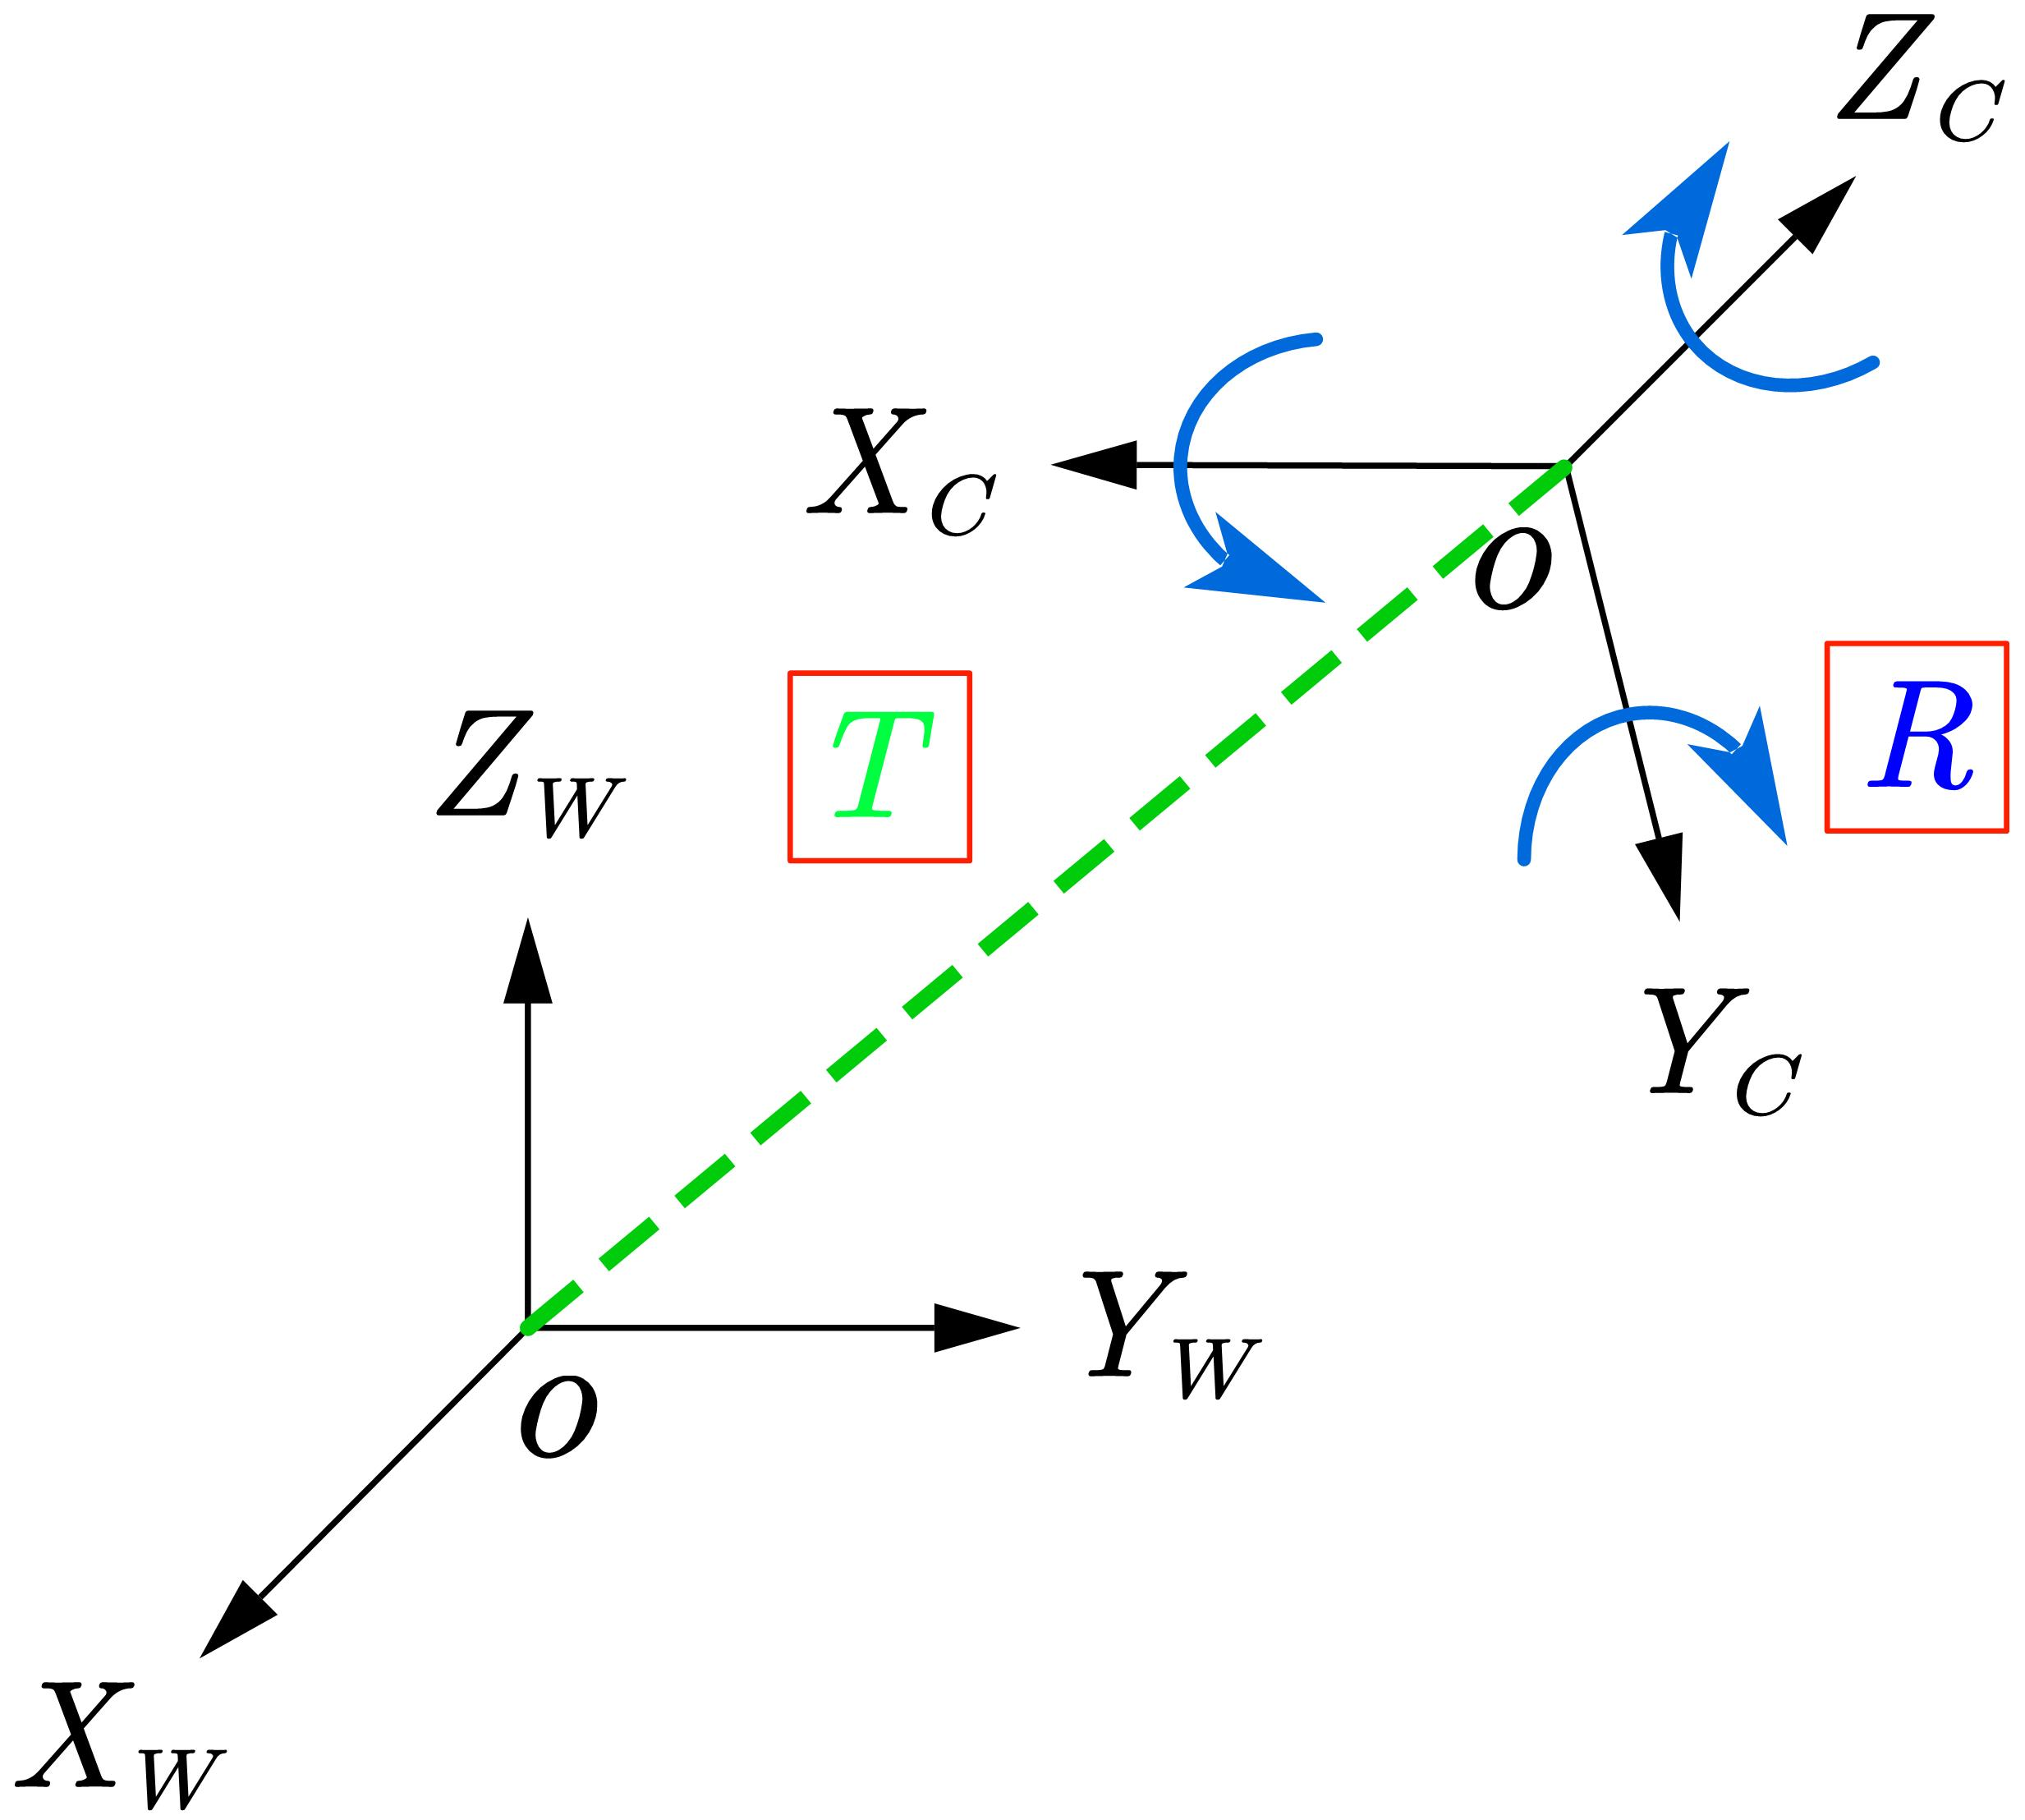
\includegraphics[scale=0.8]{世界坐标系到相机坐标系}
			\end{center}
		\end{figure}
		\column{6cm}
		\begin{itemize}
			\item $X_W,Y_W,Z_W\xrightarrow{{\color{red} \text{?}}}X_C,Y_C,Z_C$
			\item 把相机想象成刚体,刚体的位姿描述:
			\begin{itemize}
				\item 平移$T$
				\item 旋转$R$
			\end{itemize}
		\end{itemize}
		\begin{gather}
\left[ \begin{array}{c}
	X_C\\
	Y_C\\
	Z_C\\
	1\\
\end{array} \right] =\left[ \begin{matrix}
	R&		T\\
	0&		1\\
\end{matrix} \right] \left[ \begin{array}{c}
	X_W\\
	Y_W\\
	Z_W\\
	1\\
\end{array} \right] 
		\end{gather}
	\end{columns}
\end{frame}

\begin{frame}
	\frametitle{相机坐标系(3D) $\Rightarrow$图像坐标系(2D)}
	\begin{figure}
		\begin{center}
			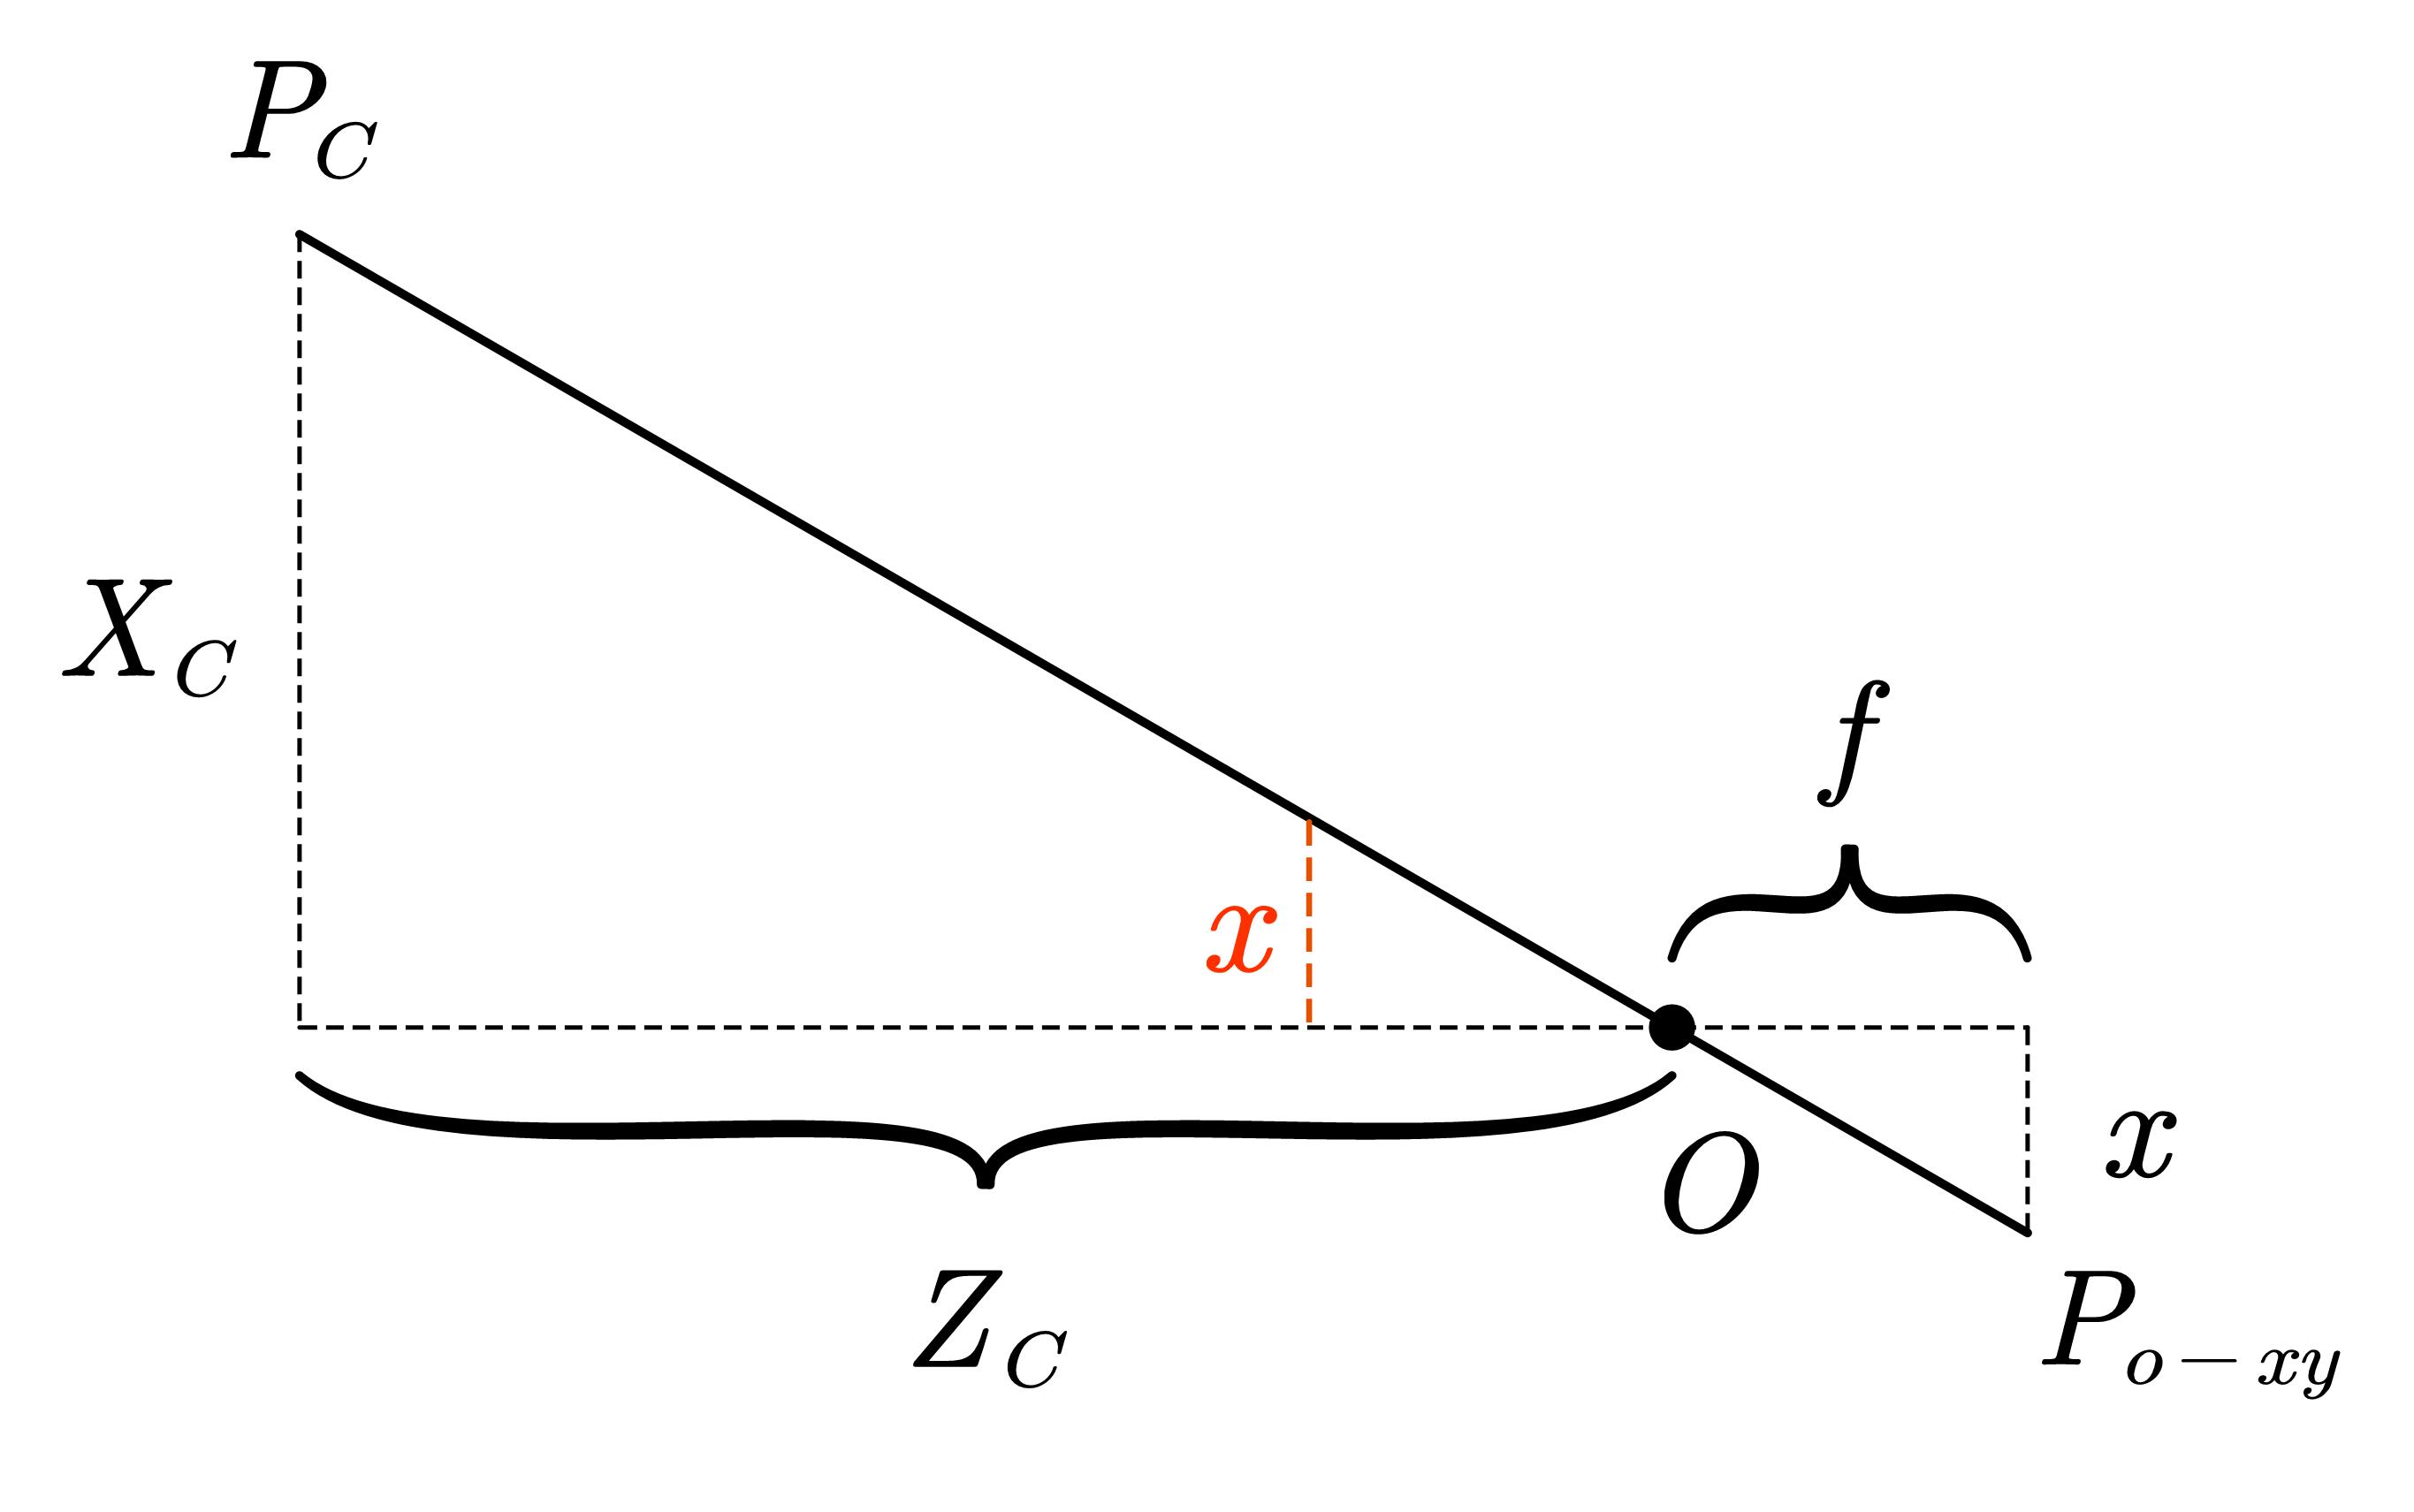
\includegraphics[scale=0.65]{小孔成像模型}
		\end{center}
	\end{figure}
	\begin{gather}
		{\small \left[ \begin{array}{c}
				x\\
				y\\
				1\\
			\end{array} \right] =\left[ \begin{matrix}
				f/Z_C&		0&		0&		0\\
				0&		f/Z_C&		0&		0\\
				0&		0&		1/Z_C&		0\\
			\end{matrix} \right] \left[ \begin{array}{c}
				X_C\\
				Y_C\\
				Z_C\\
				1\\
			\end{array} \right]   }	
	\end{gather}
	\begin{gather}
		{\small Z_C\cdot \left[ \begin{array}{c}
				x\\
				y\\
				1\\
			\end{array} \right] =\left[ \begin{matrix}
				f&		0&		0&		0\\
				0&		f&		0&		0\\
				0&		0&		1&		0\\
			\end{matrix} \right] \left[ \begin{array}{c}
				X_C\\
				Y_C\\
				Z_C\\
				1\\
			\end{array} \right]  }
	\end{gather}
\end{frame}


\begin{frame}
	\frametitle{图像坐标系(2D) $\Rightarrow$像素坐标系(2D)}
	\begin{columns}
		\column{5cm}
		\begin{figure}
			\begin{center}
				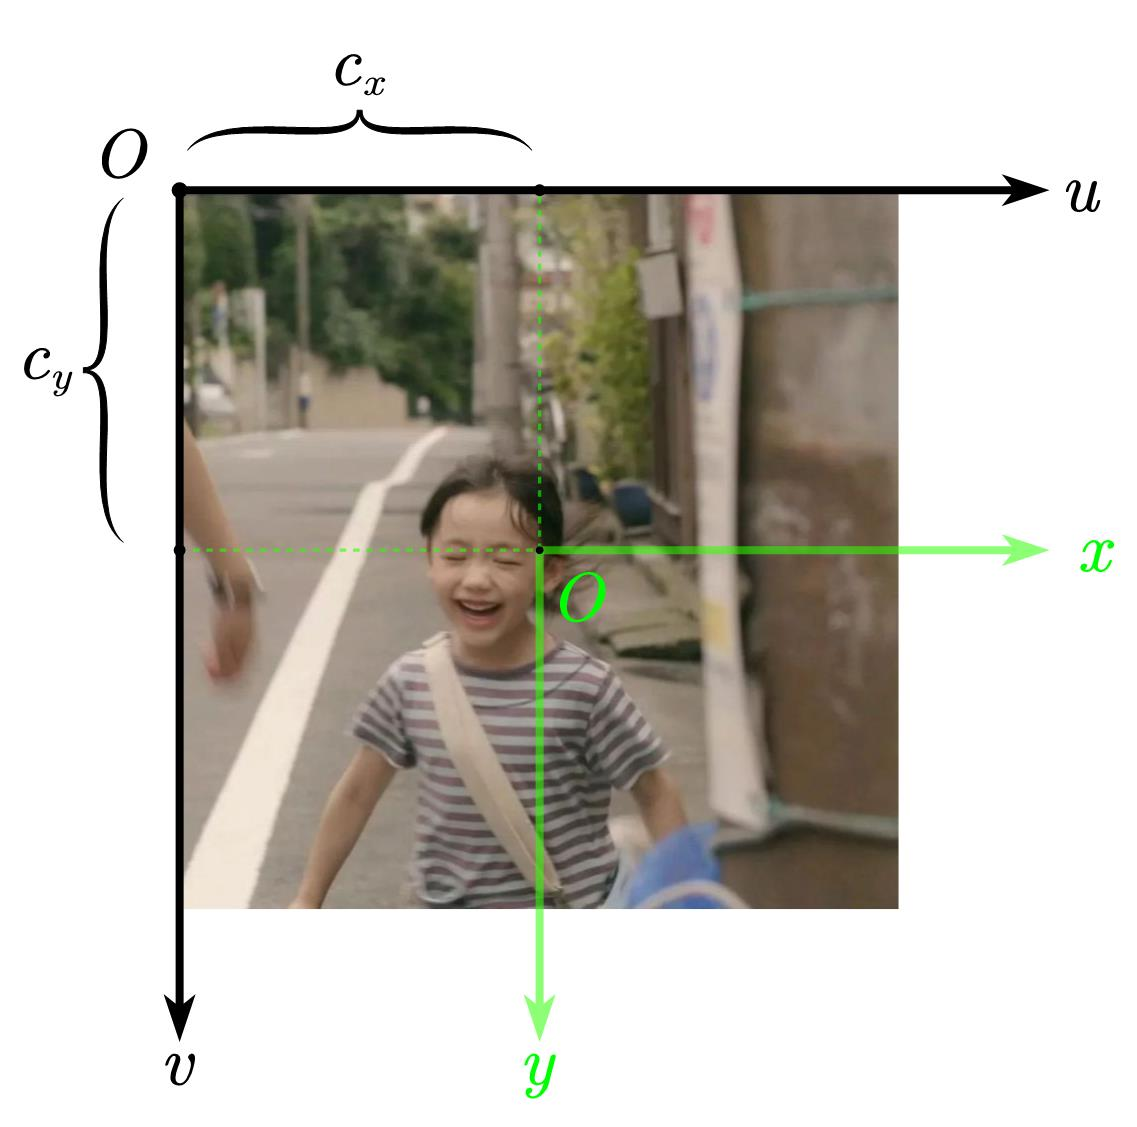
\includegraphics[scale=0.35]{相机坐标系到像素坐标系}
			\end{center}
		\end{figure}
		\column{6.5cm}
		\begin{itemize}
			\item $d_x,d_y$:像元尺寸
			\item $f_x,f_y$:各轴归一化焦距
			\vspace{-0.6em}
			$$\begin{cases}
				f_x={{f}\big/{d_x}}\\
				f_y={{f}\big/{d_y}}\\
			\end{cases}$$
			\vspace{-0.6em}
			\item $c_x$,$c_y$:两坐标系偏移量
		\end{itemize}
		\begin{gather}
			\left\{\begin{array}{c}
	u=c_x+x/d_x\\
	v=c_y+y/d_y\\
\end{array} \right
		\end{gather}
		\vspace{-0.6em}
		\begin{equation}
			\begin{aligned}
				{\small \left[ \begin{array}{c}
						u\\
						v\\
						1\\
					\end{array} \right] =\left[ \begin{matrix}
						1/d_x&		0&		c_x\\
						0&		1/d_y&		c_y\\
						0&		0&		1\\
					\end{matrix} \right] \left[ \begin{array}{c}
						x\\
						y\\
						1\\
					\end{array} \right]  }  	
			\end{aligned}	
		\end{equation}
	\end{columns}	
\end{frame}

\begin{frame}
	\frametitle{世界坐标 $\Rightarrow$像素坐标}
	\begin{small}
		\begin{equation*}
			\begin{aligned}
\left[ \begin{array}{c}
	u\\
	v\\
	1\\
\end{array} \right] &=\left[ \begin{matrix}
	1/d_x&		0&		c_x\\
	0&		1/d_y&		c_y\\
	0&		0&		1\\
\end{matrix} \right] \left[ \begin{array}{c}
	x\\
	y\\
	1\\
\end{array} \right] 
\\
&=\left[ \begin{matrix}
	1/d_x&		0&		c_x\\
	0&		1/d_y&		c_y\\
	0&		0&		1\\
\end{matrix} \right] \left[ \begin{matrix}
	f/Z_C&		0&		0&		0\\
	0&		f/Z_C&		0&		0\\
	0&		0&		1/Z_C&		0\\
\end{matrix} \right] \left[ \begin{array}{c}
	X_C\\
	Y_C\\
	Z_C\\
	1\\
\end{array} \right] 
\\
&=\left[ \begin{matrix}
	1/d_x&		0&		c_x\\
	0&		1/d_y&		c_y\\
	0&		0&		1\\
\end{matrix} \right] \left[ \begin{matrix}
	f/Z_C&		0&		0&		0\\
	0&		f/Z_C&		0&		0\\
	0&		0&		1/Z_C&		0\\
\end{matrix} \right] \left[ \begin{matrix}
	R&		T\\
	0&		1\\
\end{matrix} \right] \left[ \begin{array}{c}
	X_W\\
	Y_W\\
	Z_W\\
	1\\
\end{array} \right] 
\\
&=\frac{1}{Z_C}\cdot \left[ \begin{matrix}
	1/d_x&		0&		c_x\\
	0&		1/d_y&		c_y\\
	0&		0&		1\\
\end{matrix} \right] \cdot \left[ \begin{matrix}
	f&		0&		0&		0\\
	0&		f&		0&		0\\
	0&		0&		1&		0\\
\end{matrix} \right] \cdot \left[ \begin{matrix}
	R&		T\\
\end{matrix} \right] \cdot \left[ \begin{array}{c}
	X_W\\
	Y_W\\
	Z_W\\
	1\\
\end{array} \right] 
			\end{aligned}
		\end{equation*}
	\end{small}
\end{frame}



	\begin{frame}
	\frametitle{内参矩阵}
	\begin{gather*}
\left[ \begin{array}{c}
	u\\
	v\\
	1\\
\end{array} \right] =\frac{1}{Z_C}\cdot {\color{blue} \left[ \begin{matrix}
		1/d_x&		0&		c_x\\
		0&		1/d_y&		c_y\\
		0&		0&		1\\
	\end{matrix} \right] \cdot \left[ \begin{matrix}
		f&		0&		0&		0\\
		0&		f&		0&		0\\
		0&		0&		1&		0\\
	\end{matrix} \right] }\cdot \left[ \begin{matrix}
	R&		T\\
\end{matrix} \right] \cdot \left[ \begin{array}{c}
	X_W\\
	Y_W\\
	Z_W\\
	1\\
\end{array} \right]  
	\end{gather*}

	\begin{align}
M_1&={\color{blue} \left[ \begin{matrix}
		1/d_x&		0&		c_x\\
		0&		1/d_y&		c_y\\
		0&		0&		1\\
	\end{matrix} \right] \cdot \left[ \begin{matrix}
		f&		0&		0&		0\\
		0&		f&		0&		0\\
		0&		0&		1&		0\\
	\end{matrix} \right] } \nonumber
\\
&=\left[ \begin{matrix}
	f_x&		0&		c_x\\
	0&		f_y&		c_y\\
	0&		0&		1\\
\end{matrix} \right] \label{内参矩阵求解-内参矩阵}
	\end{align}	

	\end{frame}

	\begin{frame}
	\frametitle{外参矩阵}
	\begin{gather*}
\left[ \begin{array}{c}
	u\\
	v\\
	1\\
\end{array} \right] =\frac{1}{Z_C}\cdot M_1\cdot {\color{blue} \left[ \begin{matrix}
		R&		T\\
	\end{matrix} \right] }\cdot \left[ \begin{array}{c}
	X_W\\
	Y_W\\
	Z_W\\
	1\\
\end{array} \right] 
	\end{gather*}
	\begin{gather}
M_2={\color{blue} \left[ \begin{matrix}
		R&		T\\
	\end{matrix} \right] }
	\end{gather}
	\end{frame}


	\begin{frame}
	\frametitle{单应性矩阵\footnote{包含了相机的内外参和缩放因子,反映世界坐标系与像素坐标系之间的对应关系}(Homography Matrix)}
	\begin{columns}
	\column{7cm}
	\begin{small}

	\begin{align}
\left[ \begin{array}{c}
	u\\
	v\\
	1\\
\end{array} \right] &=\frac{1}{{\color{blue} Z_C}}\cdot M_1\cdot \left[ \begin{matrix}
	{\color{blue} r_1}&		{\color{blue} r_2}&		{\color{blue} r_3}&		T\\
\end{matrix} \right] \cdot \left[ \begin{array}{c}
	X_W\\
	Y_W\\
	{\color{blue} Z_W}\\
	1\\
\end{array} \right] \nonumber
\\
&=s \cdot M_1\cdot \left[ \begin{matrix}
	r_1&		r_2&		{\color[RGB]{255, 0, 128} r_3}&		T\\
\end{matrix} \right] \cdot \left[ \begin{array}{c}
	X_W\\
	Y_W\\
	{\color[RGB]{255, 0, 128} Z_W}\\
	1\\
\end{array} \right] \nonumber
\\
&=s \cdot M_1\cdot \left[ \begin{matrix}
	r_1&		r_2&		T\\
\end{matrix} \right] \cdot \left[ \begin{array}{c}
	X_W\\
	Y_W\\
	1\\
\end{array} \right] \nonumber
\\
&=\boldsymbol{H}\cdot \left[ \begin{array}{c}
	X_W\\
	Y_W\\
	1\\
\end{array} \right]  	\label{单应矩阵包含内外参矩阵}	
	\end{align}
	\end{small}
	\column{5.5cm}
	\begin{itemize}
		\item 棋盘格角点的$Z_W=0$
		\item 令$s ={{1}\big/{Z_C}}$,称为缩放因子
		\item 令$R=\left[ \begin{matrix}
			r_1&		r_2&		r_3\\
		\end{matrix} \right] $
	\end{itemize}	
	\end{columns}
	\end{frame}
	
	\begin{frame}
	\frametitle{齐次坐标\footnote{<Multiple view geometry in computer vision>}(Homogeneous Coordinate):目的}
	\begin{itemize}
		\item 几何变换,主要包括平移、旋转、缩放。
		\item 用矩阵来表达这些变换时,平移是矩阵相加,旋转和缩放则是矩阵相乘,$p' = m_1*p+ m_2$
		\item 综合起来表示为$p' = M*p$
	\end{itemize}
	\vspace{1em}

\quad 引入齐次坐标的目的主要是{\color[RGB]{128, 0, 255} \text{合并矩阵运算中的乘法和加法}}。
%(注:因为习惯的原因,实际使用时一般使用变化矩阵左乘向量)。
	\end{frame}

	\begin{frame}
	\frametitle{齐次坐标(Homogeneous Coordinate):问题}
	\begin{enumerate}
		\item 平行直线相交问题
		\begin{figure}
			\begin{center}
				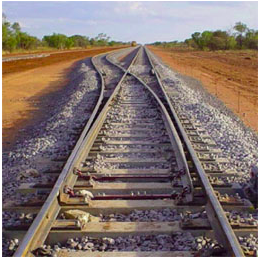
\includegraphics[scale=0.4]{平行线相交}
			\end{center}
		\end{figure}
		\begin{itemize}
		\item 欧式空间(笛卡尔空间):同一平面的平行直线不相交
		\item 透视空间:可以相交
		\end{itemize}
		\item 表示无穷远点:无穷远点$\left( \infty ,\infty \right)$在欧式空间没有意义
	\end{enumerate}
	\end{frame}

	\begin{frame}
	\frametitle{齐次坐标(Homogeneous Coordinate):解决}
	\begin{block}{使用N+1维坐标来代替N维坐标}
	\begin{equation*}
	\begin{aligned}
				\mathop {\left( x,y,w \right) \Longleftrightarrow \left( \frac{x}{w},\frac{y}{w} \right)} \limits_{\mathrm{Homogeneous}    \quad        \mathrm{Cartesian}}			
	\end{aligned}
	\end{equation*}
	\end{block}
	\begin{exampleblock}{为什么叫齐次性?\footnote{表示二维平面的无穷远点$\left( x,y,0 \right) \Longleftrightarrow \left( \infty ,\infty \right) $}}
	\begin{equation*}
	\begin{aligned}
	&	\left( 1,2,3 \right) \Rightarrow \left( \frac{1}{3},\frac{2}{3} \right) 
		\\
	&	\left( 2,4,6 \right) \Rightarrow \left( \frac{2}{6},\frac{4}{6} \right) =\left( \frac{1}{3},\frac{2}{3} \right) 
		\\
	&	\left( {\color[RGB]{0, 0, 240} a,2a,3a} \right) \Rightarrow \left( \frac{a}{3a},\frac{2a}{3a} \right) =\left( \frac{1}{3},\frac{2}{3} \right) 
	\end{aligned}	
	\end{equation*}
	\end{exampleblock}

	\end{frame}







	\begin{frame}
	\frametitle{单应性(Homography)}
	单应性是射影几何中的概念,又称为射影变换、透视变换,反映两个平面之间的映射关系。
	\begin{figure}
	\setcounter{subfigure}{0}
	\subfigure[单应性原理]
	{
		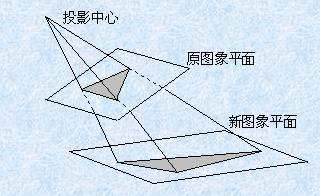
\includegraphics[scale=0.61]{射影变换}
	}
	\subfigure[不同图像上的同一点]
	{
		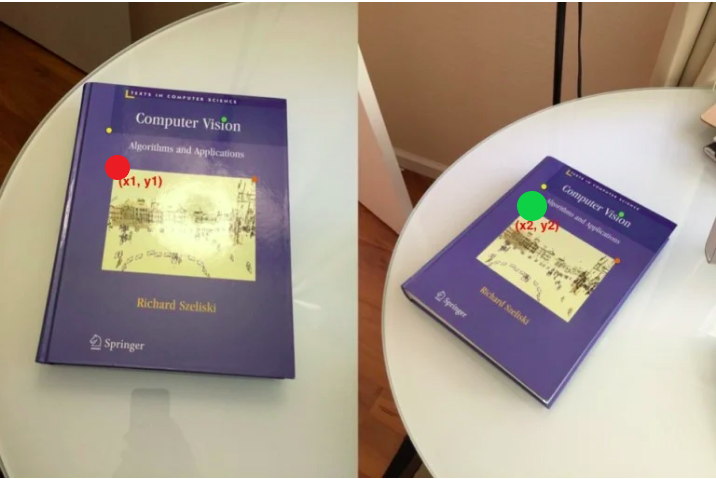
\includegraphics[scale=0.25]{单应性}
	}
\\对于现实世界的同一点,在不同视角的图像上可以用单应性矩阵来表达:
	\begin{equation}\label{单应性}
		p_2=H\cdot p_1
	\end{equation}
	\end{figure}
	\end{frame}




	\begin{frame}
	\frametitle{单应性矩阵应用}
	\begin{itemize}
		\item 图像校正
		\item 图像拼接
		\item 相机位姿估计
		\item 视觉SLAM
		\item 增强现实(AR)
	\end{itemize}
	\end{frame}


	
	
	




	
%	\subsection{利用SIFT(尺度不变特征变换)算法提取特征点}
%	
%	\begin{frame}
%	\frametitle{关于SIFT算法\footnote{版权属于英属哥伦比亚大学}}
%
%	\begin{figure}[htbp]
%	\setcounter{subfigure}{0} %子图重新编号
%	\subfigure[David lowe]
%	{
%		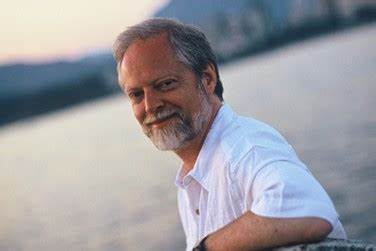
\includegraphics[scale=0.325]{David lowe}
%	}	
%	\subfigure[特征点匹配]
%	{
%		
\includegraphics[scale=0.23]{SIFT算法示意}
%	}
%	\end{figure}
%	\begin{itemize}
%		\item 拍摄全景图片
%	\end{itemize}
%	\end{frame}
%
%	\begin{frame}
%	\frametitle{一、建立高斯差分金字塔}
%	\begin{figure}
%	\begin{center}
%		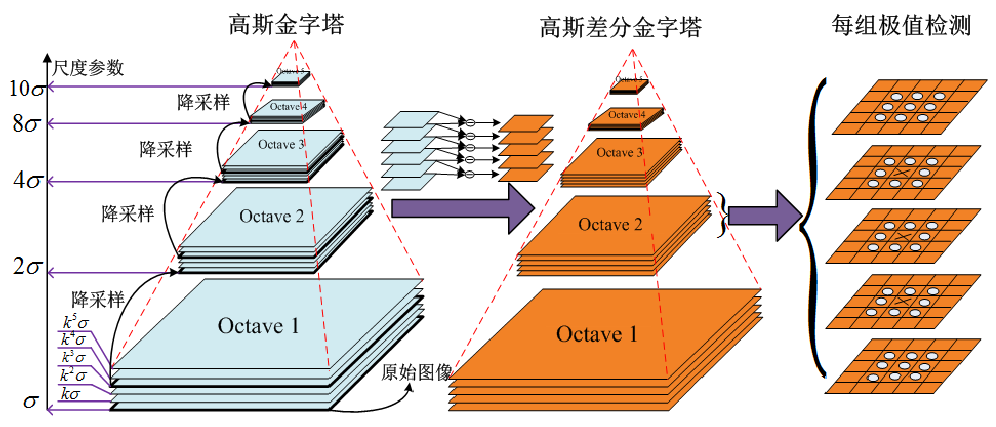
\includegraphics[scale=0.35]{高斯差分金字塔1}
%		\caption{高斯差分金字塔建立过程}
%	\end{center}
%	\end{figure}
%	\end{frame}
%
%	\begin{frame}
%	\frametitle{一、建立高斯差分金字塔:(1)分组,分层}
%	\begin{figure}
%	\begin{center}
%		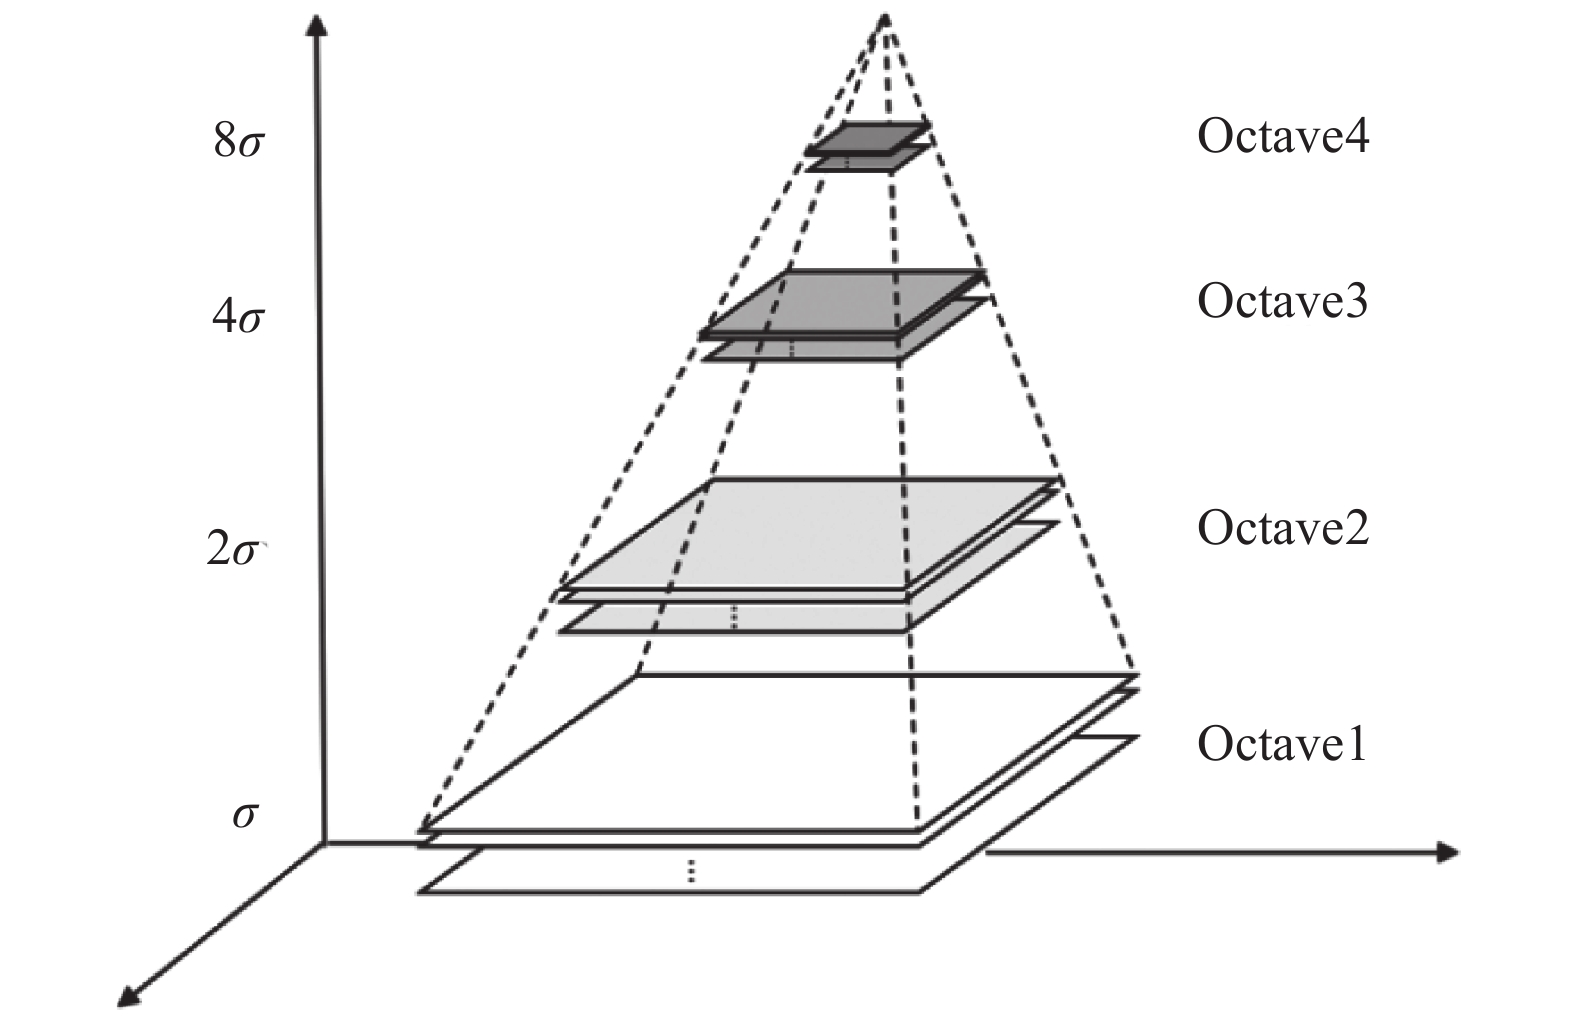
\includegraphics[scale=0.7]{高斯差分金字塔2}
%		\caption{高斯金字塔-组,层}
%	\end{center}
%	\end{figure}
%	\begin{block}{(1)分组,分层\footnote{<Object recognition from local scale-invariant features-David Lowe>}}
%		\begin{itemize}
%			\item 组:$O=\left[ \log _2\left( \min \left( M,N \right) \right) \right] -3$,$M,N$分别是图像的宽和高
%			\item 层:$S=n+3$
%		\end{itemize}
%	\end{block}
%	\end{frame}
%
%	\begin{frame}
%	\frametitle{一、建立高斯差分金字塔:(2)降采样,高斯模糊}
%	\begin{figure}
%	\setcounter{subfigure}{0} %子图重新编号
%	\subfigure[高斯金字塔-不同尺度的高斯模糊]
%	{
%		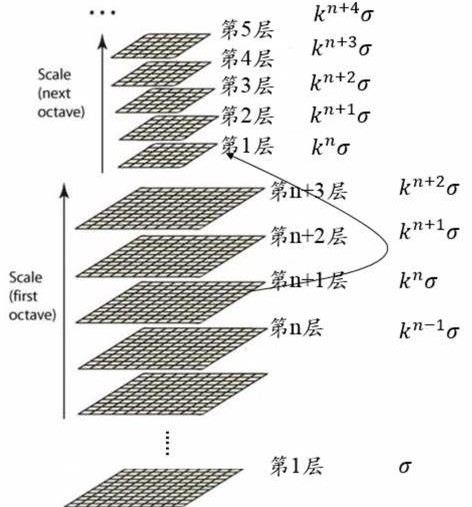
\includegraphics[scale=0.25]{高斯差分金字塔3}
%	}
%	\subfigure[不同尺度模拟近大远小]
%	{
%		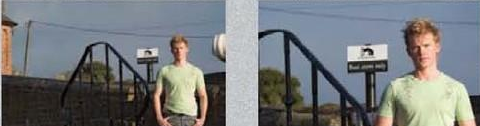
\includegraphics[scale=0.45]{同一物体不同距离-高斯模糊}
%	}
%	\end{figure}
%	\vspace{-0.6em}
%	\begin{block}{(2)降采样、高斯模糊}
%		\begin{itemize}
%			\item $k=2^{\frac{1}{n}}$
%			\item $\sigma =1.52$
%		\end{itemize}
%	\end{block}
%
%	\end{frame}
%
%	\begin{frame}
%	\frametitle{一、建立高斯差分金字塔:(3)对卷积后的层作差分}
%	\begin{columns}
%		\column{5cm}
%		\begin{figure}
%			\begin{center}
%				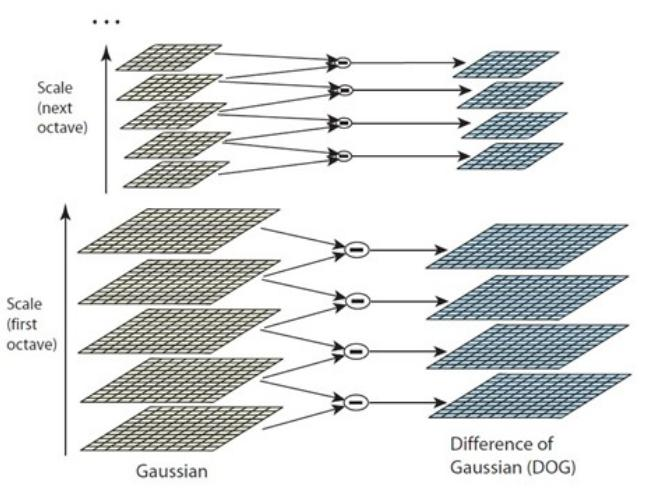
\includegraphics[scale=0.25]{高斯差分金字塔4}
%				\caption{高斯差分金字塔}
%			\end{center}
%		\end{figure}
%		\column{5.5cm}
%		\begin{block}{(3)对卷积后的层相减}
%			\begin{itemize}
%				\item 去掉顶层和底层,只有$n=S-3$层能用于特征点提取
%				\item 这样我们就建立起了高斯差分金字塔:Difference of Gaussian(DOG)
%			\end{itemize}
%		\end{block}
%	\end{columns}
%	\end{frame}
%
%
%	\begin{frame}
%	\frametitle{二、确定关键点\footnote{关键点,也称兴趣点、特征点}位置:(1)在差分金字塔中寻找极值}
%	\begin{figure}
%	\setcounter{subfigure}{0} %子图重新编号
%	\subfigure[三个方向确定极值]
%	{
%		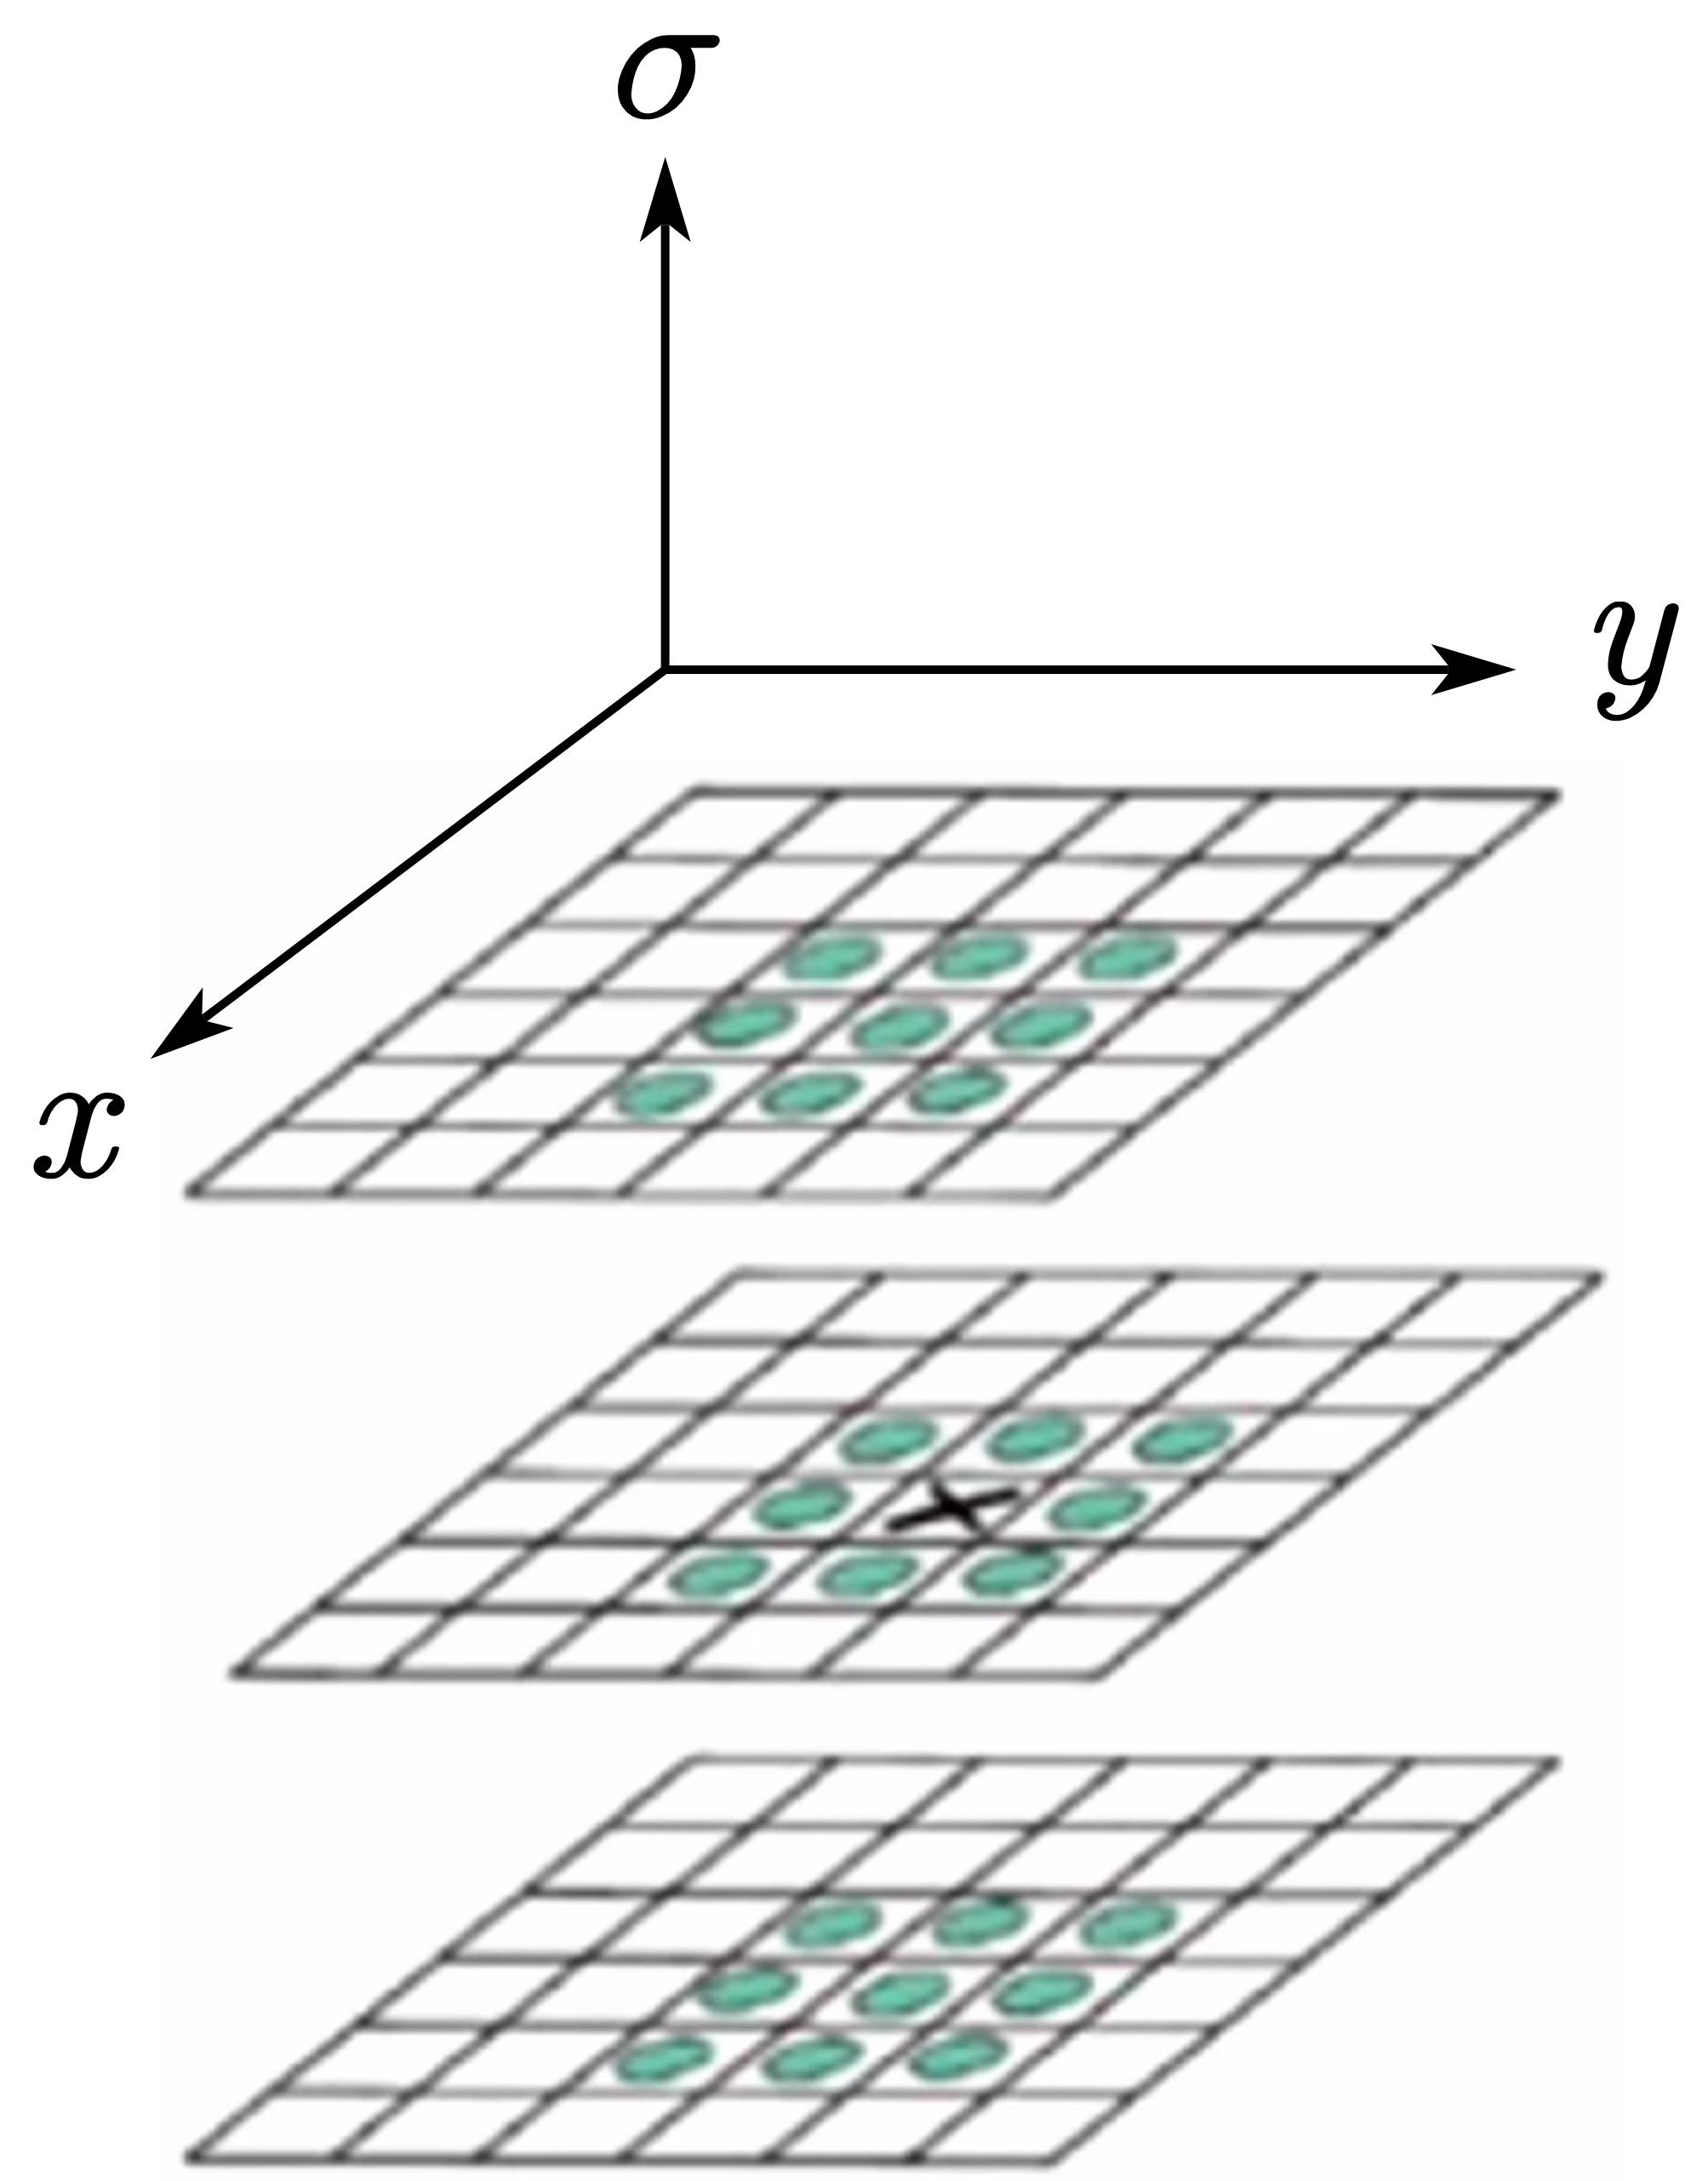
\includegraphics[scale=0.6]{确定关键点位置三维空间}
%	}
%	\subfigure[理论与实际位置]
%	{
%		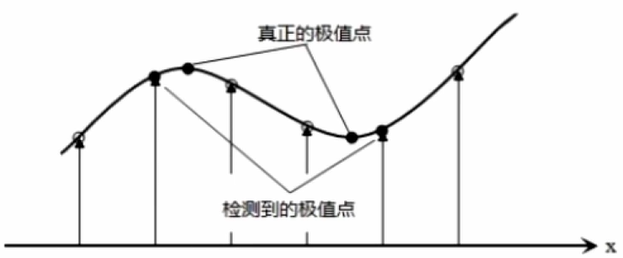
\includegraphics[scale=0.3]{SIFT-确定关键点位置2}
%	}
%	\end{figure}
%
%	\end{frame}
%
%
%
%	\begin{frame}
%	\frametitle{二、确定关键点位置:(1)在差分金字塔中寻找极值}
%	\begin{exampleblock}{Example:一元泰勒展开}
%		令	
%		\vspace{-0.6em} 
%		\begin{small}
%			\begin{align}
%				f\left( x \right) ={\color{blue} f\left( x_0 \right) +f'\left( x_0 \right) \left( x-x_0 \right) +\frac{1}{2}f''\left( x_0 \right) \left( x-x_0 \right) ^2}+\cdots  \label{SIFT-确定关键点位置-一元泰勒展开}
%			\end{align}
%		\end{small}
%	式(\ref{SIFT-确定关键点位置-一元泰勒展开})两边同时求导,得:
%	\vspace{-0.6em}
%	\begin{small}
%	\begin{align}
%		f'\left( x \right) ={\color[RGB]{64, 0, 0} f'\left( x_0 \right) +f''\left( x_0 \right) \left( x-x_0 \right) } \label{SIFT-确定关键点位置-一元泰勒展开求导}
%	\end{align} 
%	\end{small}
%	令式(\ref{SIFT-确定关键点位置-一元泰勒展开求导})两边同时为0,得:
%	\vspace{-0.6em}
%	\begin{small}
%		\begin{align}
%			x=-\frac{f'\left( \begin{array}{c}
%					x_0\\
%				\end{array} \right)}{f''\left( \begin{array}{c}
%					x_0\\
%				\end{array} \right)}+x_0 \label{SIFT-确定关键点位置-一元泰勒展开求导-解}
%		\end{align} 
%	\end{small}
%	对式(\ref{SIFT-确定关键点位置-一元泰勒展开求导-解})进行牛顿迭代得:
%	\vspace{-0.6em}
%	\begin{small}
%		\begin{align}
%			x_{n+1}=x_n-\frac{f'\left( x_n \right)}{f''\left( \begin{array}{c}
%					x_n\\
%				\end{array} \right)}
%		\end{align}
%	\end{small}
%	\end{exampleblock}
%	\end{frame}
%
%	\begin{frame}
%	\frametitle{确定关键点位置:高维泰勒展开}
%	\begin{block}{(1)高维泰勒展开及牛顿迭代确定关键点位置}
%			\begin{align}
%			f\left( x,y,\sigma \right) =f\left( x_0,y_0,\sigma _0 \right) +\left( \frac{\alpha f}{\alpha x},\frac{\alpha f}{\alpha y},\frac{\alpha f}{\alpha \sigma} \right) \cdot \left( \begin{array}{c}
%				x-x_0\\
%				y-y_0\\
%				\sigma -\sigma _0\\
%			\end{array} \right) + \nonumber
%			\\
%			\frac{1}{2} \left( \begin{array}{c}
%				x-x_0\\
%				y-y_0\\
%				\sigma -\sigma _0\\
%			\end{array} \right) ^T\left( \begin{matrix}
%				\frac{\alpha ^2f}{\alpha x^2}&		\frac{\alpha ^2f}{\alpha x\alpha y}&		\frac{\alpha ^2f}{\alpha x\alpha \sigma}\\
%				\frac{\alpha ^2f}{\alpha x\alpha y}&		\frac{\alpha ^2f}{\alpha y^2}&		\frac{\alpha ^2f}{\alpha y\alpha \sigma}\\
%				\frac{\alpha ^2f}{\alpha x\alpha \sigma}&		\frac{\alpha ^2f}{\alpha y\alpha \sigma}&		\frac{\alpha ^2f}{\alpha \sigma ^2}\\
%			\end{matrix} \right) \left( \begin{array}{c}
%				x-x_0\\
%				y-y_0\\
%				\sigma -\sigma _0\\
%			\end{array} \right) \nonumber
%		\end{align}
%		令$X=\left( x,y,\sigma \right) ^T$,上式化简为:
%		\begin{small}
%			\begin{align}
%				f\left( X \right) =f\left( X_0 \right) +\frac{\alpha f^T}{\alpha X}\widehat{X}+\frac{1}{2}\widehat{X}^T\frac{\alpha ^2f^T}{\alpha X^2}\widehat{X} \nonumber
%			\end{align}
%		\end{small}
%		求导、令导数为0、牛顿迭代。
%	\end{block}
%	\end{frame}
%
%
%	\begin{frame}
%	\frametitle{确定关键点方向}
%	
%	\end{frame}
%
%	\begin{frame}
%	\frametitle{确定关键点描述符}
%	
%	\end{frame}






	\subsection{张正友标定法:求解内外参及单应矩阵}
	
	\begin{frame}
	\frametitle{相机标定目的}
	   \quad 其中相机的内参和外参可以通过张正友标定法获取。通过最终的转换关系来看,一个三维中的坐标点,的确可以在图像中找到一个对应的像素点,但是反过来,通过图像中的一个点找到它在三维中对应的点就很成了一个问题,因为我们并不知道等式左边的$Z_C$的值。
	\end{frame}
	
	
	
		\begin{frame}
		\frametitle{单应性矩阵的求解}
		\begin{block}{(1)齐次坐标}
			令$p_1=\left( x_1,y_1 \right) ^T,p_2=\left( x_2,y_2 \right) ^T,H=\left[ \begin{matrix}
				h_{11}&		h_{12}&		h_{13}\\
				h_{21}&		h_{22}&		h_{23}\\
				h_{31}&		h_{32}&		h_{33}\\
			\end{matrix} \right] =\left[ \begin{matrix}
				h_1&		h_2&		h_3\\
			\end{matrix} \right]  $,$H$把$p_1$映射到$p_2$,对应齐次坐标为:$p_1=\left( x_1,y_1,1 \right) ^T,p_2=\left( x_2,y_2,1 \right) ^T$
		\end{block}
		\begin{block}{(2)单应性矩阵的自由度}
			在等式(\ref{单应性})两端同时乘以常数$a$原等式化为$a\cdot p_2={\color{blue} a\cdot H}\cdot p_1$,新得到的单应性矩阵$aH$和原单应性矩阵$H$的作用相同,因为齐次坐标乘以常数后保持不变,所以虽然$H$有九个元素,但自由度却为8,我们常令$h_{33}=1$以简化计算。
		\end{block}
	\end{frame}
	
	\begin{frame}
		\frametitle{单应性矩阵的求解}
		%	\begin{small}
			
			\begin{align}
				\left[ \begin{array}{c}
					x_2\\
					y_2\\
					1\\
				\end{array} \right] &=\left[ \begin{matrix}
					h_{11}&		h_{12}&		h_{13}\\
					h_{21}&		h_{22}&		h_{23}\\
					h_{31}&		h_{32}&		h_{33}\\
				\end{matrix} \right] \cdot \left[ \begin{array}{c}
					x_1\\
					y_1\\
					1\\
				\end{array} \right] \nonumber
				\\
				& \Rightarrow \begin{cases}
					x_2=h_{11}\cdot x_1+h_{12}\cdot y_1+h_{13}\\
					y_2=h_{21}\cdot x_1+h_{22}\cdot y_1+h_{23}\\
					1=h_{31}\cdot x_1+h_{32}\cdot y_1+h_{33}\\
				\end{cases}\Rightarrow \begin{cases}
					x_2=\frac{h_{11}\cdot x_1+h_{12}\cdot y_1+h_{13}}{h_{31}\cdot x_1+h_{32}\cdot y_1+h_{33}}\\
					y_2=\frac{h_{21}\cdot x_1+h_{22}\cdot y_1+h_{23}}{h_{31}\cdot x_1+h_{32}\cdot y_1+h_{33}}\\
				\end{cases} \nonumber
				\\
				& \Rightarrow \begin{cases}
					x_2\left( h_{31}\cdot x_1+h_{32}\cdot y_1+h_{33} \right) -\left( h_{11}\cdot x_1+h_{12}\cdot y_1+h_{13} \right) =0\\
					y_2\left( h_{31}\cdot x_1+h_{32}\cdot y_1+h_{33} \right) -\left( h_{21}\cdot x_1+h_{22}\cdot y_1+h_{23} \right) =0\\
				\end{cases} \nonumber
				\\
				& \Rightarrow \begin{cases}
					-h_{11}\cdot x_1-h_{12}\cdot y_1-h_{13}+h_{31}\cdot x_1x_2+h_{32}\cdot y_1+h_{33}=0\\
					-h_{21}\cdot x_1-h_{22}\cdot y_1-h_{23}+h_{31}\cdot x_1y_2+h_{32}\cdot y_1+h_{33}=0\\
				\end{cases}  \nonumber \\
				& \Rightarrow A\cdot h=\boldsymbol{0} \label{线性解法}
			\end{align}	
			
			%	\end{small}
	\end{frame}
	
	\begin{frame}
		\frametitle{单应性矩阵的求解}
		\begin{block}{(3)求解单应矩阵}
			\begin{itemize}
				\item $A=\left[ \begin{matrix}
					x_1&		y_1&		1&		0&		0&		0&		x_1x_2&		y_1&		1\\
					0&		0&		0&		x_1&		y_1&		1&		x_1y_2&		y_1&		1\\
				\end{matrix} \right] $
				\item $h=\left[ \begin{matrix}
					h_{11}&		h_{12}&		h_{13}&		h_{21}&		h_{22}&		h_{23}&		h_{31}&		h_{32}&		{\color[RGB]{0, 0, 240} h_{33}}\\
				\end{matrix} \right] ^T$
				\vspace{0.8em}
				\item 棋盘格一个脚点对应两个方程,对应$A$矩阵的两行,所以只需四个脚点就可以将$A$垒到八行,$A\cdot h=\boldsymbol{0}$就存在唯一解。
			\end{itemize}
		\end{block}
	\end{frame}
	
	
	\begin{frame}
		\frametitle{单应性矩阵的求解}
		\begin{block}{(4)理想与现实}
			\begin{itemize}
				\item 以上只是理论的推导,在真实的场景中,我们计算的点中都会包含噪声。比如点的位置偏差几个像素,甚至出现特征点对误匹配的现象,如果仅用四个点对来计算单应矩阵,那么会出现很大的误差。
				\item  因此为了计算的更加准确,一般采用远大于4个点来计算单应矩阵,假如有$n$对,$A$矩阵将垒到$2n$行,此时用最小二乘法、随机采样一致性$(RANSAC)$、$SVD$分解就可以求解$h(H)$。
				\item 如果方程\ref{线性解法}采用线性解法很难得到最优解,所以一般采取其它的优化方法如SVD奇异值分解、Levenberg-Marquarat(LM)算法等进行求解。
			\end{itemize}
		\end{block}
	\end{frame}
	
	\begin{frame}
		\frametitle{内参矩阵的求解:不考虑畸变}
		\begin{itemize}
			\item 求解思路是利用旋转向量的约束关系
			\item 单应矩阵包括内参和外参矩阵,而内参矩阵更方便求解,之后再求外参矩阵。
			根据式(\ref{单应矩阵包含内外参矩阵}),我们可以得到以下关系:\\
			\begin{align}
				H &=\left[ \begin{matrix}
					h_1&		h_2&		h_3\\
				\end{matrix} \right] \nonumber
				\\
				&=s \cdot M_1\cdot M_2 \nonumber
				\\
				&=s \cdot M_1\cdot \left[ \begin{matrix}
					r_1&		r_2&		T\\
				\end{matrix} \right] \nonumber
				\\
				&	\Rightarrow \begin{cases}
					h_1=sM_1r_1\\
					h_2=sM_1r_2\\
					h_3=sM_1T\\
				\end{cases} \nonumber
				\\
				&	\Rightarrow \begin{cases}
					r_1=s ^{-1} {M_1}^{-1}h_1\\
					r_2=s ^{-1} {M_1}^{-1}h_2\\
					T=s ^{-1} {M_1}^{-1}h_3\\
				\end{cases}
			\end{align}
		\end{itemize}
	\end{frame}	
	
	\begin{frame}
		\frametitle{内参矩阵的求解:不考虑畸变}
		\begin{block}{约束条件1:旋转向量正交}
			\begin{small}
				\begin{align}
					& {r_1}^Tr_2=0 \nonumber
					\\
					& \Rightarrow {h_1}^T{\color{blue} \left( s ^{-1} {M_1}^{-1} \right) ^Ts ^{-1} {M{\color{blue} _1}}^{-1}}h_2=0 \label{内参矩阵的求解约束条件1}
				\end{align}
			\end{small}
		\end{block}
		
		\begin{block}{约束条件2:旋转向量长度相等(旋转不改变尺度)}
			\begin{small}
				\begin{align}
					& \left\| r_1 \right\| =\left\| r_2 \right\| =1 \nonumber
					\\
					& \Rightarrow {r_1}^Tr_1={r_2}^Tr_2 \nonumber
					\\
					& \Rightarrow {h_1}^T{\color{blue} \left( s ^{-1}{M_1}^{-1} \right) ^Ts ^{-1}{M{\color{blue} _1}}^{-1}}h_1={h_2}^T{\color{blue} \left( s ^{-1}{M_1}^{-1} \right) ^Ts ^{-1}{M{\color{blue} _1}}^{-1}}h_2 \label{内参矩阵的求解约束条件2}
				\end{align}
			\end{small}
		\end{block}
	\end{frame}	
	
	\begin{frame}
		\frametitle{内参矩阵的求解:不考虑畸变}
		令$M_1=\left[ \begin{matrix}
			f_x&		{\color{blue} \gamma\footnote{畸变因子,非常小,一般忽略} }&		c_x\\
			0&		f_y&		c_y\\
			0&		0&		1\\
		\end{matrix} \right] $,再令$B={\color{blue} \left( s ^{-1}{M_1}^{-1} \right) ^Ts ^{-1}{M{\color{blue} _1}}^{-1}}$,我们得到:\\
		\begin{align}
			B&=\left( s^{-1}{M_1}^{-1} \right) ^Ts^{-1}{M_1}^{-1}={\color{blue} \lambda }\left( {M_1}^{-1} \right) ^T{M_1}^{-1} \label{内参矩阵的求解-B矩阵}
			\\
			&=\lambda \cdot\left[ \begin{matrix}
				\frac{1}{{f_x}^2}&		-\frac{\gamma}{{f_x}^2f_y}&		\frac{c_y\gamma -c_xf_y}{{f_x}^2f_y}\\
				-\frac{\gamma}{{f_x}^2f_y}&		\frac{\gamma ^2}{{f_x}^2{f_y}^2}+\frac{1}{{f_y}^2}&		-\gamma \frac{c_y\gamma -c_xf_y}{{f_x}^2{f_y}^2}-\frac{c_y}{{f_y}^2}\\
				\frac{c_y\gamma -c_xf_y}{{f_x}^2f_y}&		-\gamma \frac{c_y\gamma -c_xf_y}{{f_x}^2{f_y}^2}-\frac{c_y}{{f_y}^2}&		\frac{\left( c_y\gamma -c_xf_y \right) ^2}{{f_x}^2{f_y}^2}+\frac{{c_y}^2}{{f_y}^2}+1\\
			\end{matrix} \right] \nonumber
			\\
			&	=\left[ \begin{matrix}
				b_{11}&		b_{12}&		b_{13}\\
				b_{21}&		b_{22}&		b_{23}\\
				b_{31}&		b_{32}&		b_{33}\\
			\end{matrix} \right] \nonumber
		\end{align}\\
		$B$为对称阵,真正有用的元素只有6个。
	\end{frame}	
	
	\begin{frame}
		\frametitle{内参矩阵的求解:不考虑畸变}
		\begin{itemize}
			\item 	根据约束条件(\ref{内参矩阵的求解约束条件1})(\ref{内参矩阵的求解约束条件2})及式(\ref{内参矩阵的求解-B矩阵}),我们得到:\\
			\begin{align}
				\begin{cases}
					{h_1}^TBh_2=0\\
					{h_1}^TBh_1={h_2}^TBh_2\\
				\end{cases}\Leftrightarrow {h_i}^TBh_j \label{内参矩阵的求解-H矩阵的化简}
			\end{align}
			\item 令$H=\left[ \begin{matrix}
				h_1&		h_2&		h_3\\
			\end{matrix} \right] $的第$i$列列向量:$h_i=\left[ \begin{matrix}
				h_{1i}&		h_{2i}&		h_{3i}\\
			\end{matrix} \right] ^T$
			\item 将$h_i$代入式(\ref{内参矩阵的求解-H矩阵的化简})进一步化简	
		\end{itemize}
	\end{frame}	
	
	\begin{frame}
		\frametitle{内参矩阵的求解:不考虑畸变}
		\begin{align}
			{h_i}^TBh_j&=\left[ \begin{matrix}
				h_{1i}&		h_{2i}&		h_{3i}\\
			\end{matrix} \right] _{1\times 3}\cdot \left[ \begin{matrix}
				{\color{blue} b_{11}}&		b_{12}&		b_{13}\\
				{\color{blue} b_{21}}&		{\color{blue} b_{22}}&		b_{23}\\
				{\color{blue} b_{31}}&		{\color{blue} b_{32}}&		{\color{blue} b_{33}}\\
			\end{matrix} \right] _{3\times 3}\cdot \left[ \begin{array}{c}
				h_{1j}\\
				h_{2j}\\
				h_{3j}\\
			\end{array} \right] _{3\times 1} \nonumber
			\\
			&	={\left[ \begin{array}{c}
					h_{1i}\cdot b_{11}+h_{2i}\cdot b_{21}+h_{3i}\cdot b_{31}\\
					h_{1i}\cdot b_{12}+h_{2i}\cdot b_{22}+h_{3i}\cdot b_{32}\\
					h_{1i}\cdot b_{13}+h_{2i}\cdot b_{23}+h_{3i}\cdot b_{33}\\
				\end{array} \right] _{{\color[RGB]{240, 0, 0} 1}\times 3}}^T\cdot \left[ \begin{array}{c}
				h_{1j}\\
				h_{2j}\\
				h_{3j}\\
			\end{array} \right] _{3\times {\color[RGB]{240, 0, 0} 1}} \nonumber
			\\
			&	=\left[ \begin{array}{c}
				h_{1i}h_{1j}\\
				h_{1j}h_{2i}+h_{2j}h_{1i}\\
				h_{2i}h_{2j}\\
				h_{1j}h_{3i}+h_{3j}h_{1i}\\
				h_{3i}h_{3j}\\
				h_{2j}h_{3i}+h_{3j}h_{2i}\\
			\end{array} \right] ^T\left[ \begin{array}{c}
				b_{11}\\
				b_{12}\\
				b_{22}\\
				b_{13}\\
				b_{33}\\
				b_{23}\\
			\end{array} \right] \label{内参矩阵的求解-hb-vb代换}
		\end{align}
	\end{frame}	
	
	\begin{frame}
		\frametitle{内参矩阵的求解:不考虑畸变}
		在式(\ref{内参矩阵的求解-hb-vb代换})中,令:\\
		\begin{align}
			v_{ij}&=\left[ \begin{array}{c}
				h_{1i}h_{1j}\\
				h_{1j}h_{2i}+h_{2j}h_{1i}\\
				h_{2i}h_{2j}\\
				h_{1j}h_{3i}+h_{3j}h_{1i}\\
				h_{3i}h_{3j}\\
				h_{2j}h_{3i}+h_{3j}h_{2i}\\
			\end{array} \right] ^T
			\\
			b&=\left[ \begin{array}{c}
				b_{11}\\
				b_{12}\\
				b_{22}\\
				b_{13}\\
				b_{33}\\
				b_{23}\\
			\end{array} \right] \label{内参矩阵求解-b}
		\end{align}
	\end{frame}	
	
	
	\begin{frame}
		\frametitle{内参矩阵的求解:不考虑畸变}
		根据式(\ref{内参矩阵的求解-H矩阵的化简}),得到:\\
		\begin{align}
			\begin{cases}\label{内参矩阵求解-每张图片都可以得到两个等式}
				{v_{12}}^Tb=0\\
				\left( {v_{11}}^T-{v_{22}}^T \right) b\\
			\end{cases}
		\end{align}进一步整理得到:
		\begin{align}\label{内参矩阵求解-每张图片将矩阵垒两行}
			\left[ \begin{array}{c}
				{v_{12}}^T\\
				{v_{11}}^T-{v_{22}}^T\\
			\end{array} \right] \cdot b=0
		\end{align}
		\begin{shaded}
			\quad 可以用之前求解的单应矩阵$H$来得到$v_{11},v_{12},v_{22}$,并且每张图片都可以得到如如式(\ref{内参矩阵求解-每张图片都可以得到两个等式})的两个等式,可以将式(\ref{内参矩阵求解-每张图片将矩阵垒两行})中的矩阵垒两行,而如式(\ref{内参矩阵求解-b})所示,$b$只含有6个未知数,因此至少保证图片数大于等于3张才能解出$b$。
		\end{shaded}
	\end{frame}	
	
	\begin{frame}
		\frametitle{内参矩阵的求解:不考虑畸变}
		根据式(\ref{内参矩阵求解-每张图片将矩阵垒两行})求出的$b$,我们就可以得到$B$,而根据式(\ref{内参矩阵的求解-B矩阵}),我们有:\\
		\begin{align}
			\begin{cases}
				f_x=\sqrt{{{\lambda}\big/{b_{11}}}}\\ \nonumber
				f_y=\sqrt{{{\lambda b_{11}}\big/{\left( b_{11}b_{22}-{b_{12}}^2 \right)}}}\\ \nonumber
				c_x={{\gamma  c_y}\big/{f_y}}-{{b_{13}f_x}\big/{\lambda}}\\ \nonumber
				c_y={{\left( b_{12}b_{13}-b_{11}b_{23} \nonumber \right)}\big/{\left( b_{11}b_{22}-{b_{12}}^2 \right)}}\\
				\gamma =-{{b_{12}{f_x}^2f_y}\big/{\lambda}}\\ \nonumber
				\lambda =b_{33}-{{\left[ {b_{13}}^2+c_y\left( b_{12}b_{13}-b_{11}b_{23} \right) \right]}\big/{b_{11}}} \nonumber
			\end{cases}
		\end{align}
		%	\begin{shaded}
			代入式(\ref{内参矩阵求解-内参矩阵}),我们就求出了内参矩阵$M_1=\left[ \begin{matrix}
				f_x&		\gamma&		c_x\\
				0&		f_y&		c_y\\
				0&		0&		1\\
			\end{matrix} \right] $
			%	\begin{align}
				
				%	\end{align}
			%	\end{shaded}
		
	\end{frame}	
	
	
	
	
	\begin{frame}
		\frametitle{外参矩阵的求解:不考虑畸变}
		此时根据求得的内参矩阵$M_1$和单应矩阵$H$,可以根据下面两个约束条件继续求得外参矩阵$M_2$:
		\begin{block}{(1)旋转向量互相垂直}
			\begin{align}
				\begin{cases}
					r_1=s^{-1}{M_1}^{-1}h_1\\ \nonumber
					r_1=s^{-1}{M_1}^{-1}h_2\\ \nonumber
					r_3=r_1\times r_2\\ \nonumber
					T=s^{-1}{M_1}^{-1}h_3 \nonumber
				\end{cases}
			\end{align}
		\end{block}
		\begin{block}{(2)旋转向量长度为1}
			\begin{align}
				\left\| r_1 \right\| =\left\| s^{-1}{M_1}^{-1}h_1 \right\| =1 \nonumber
			\end{align}
		\end{block}
	\end{frame}	
	




%		\begin{frame}
	%			\frametitle{学科的区别和联系}
	%			\begin{itemize}
		%				\item 机器视觉
		%				\item 计算机视觉
		%				\item 计算机图形学			
		%			\end{itemize}
	%		\end{frame}	



	\subsection{单目相机标定求解左右相机内外参矩阵}

	\begin{frame}
		\frametitle{Harris corner detection:角点检测}
	\end{frame}



	\subsection{双目相机标定求解左右相机位姿关系}
	
		\begin{frame}
		\frametitle{参数求解:单目相机\footnote{单目相机不可能求出深度信息}}
		\begin{columns}
			\column{5cm}
			\begin{center}
				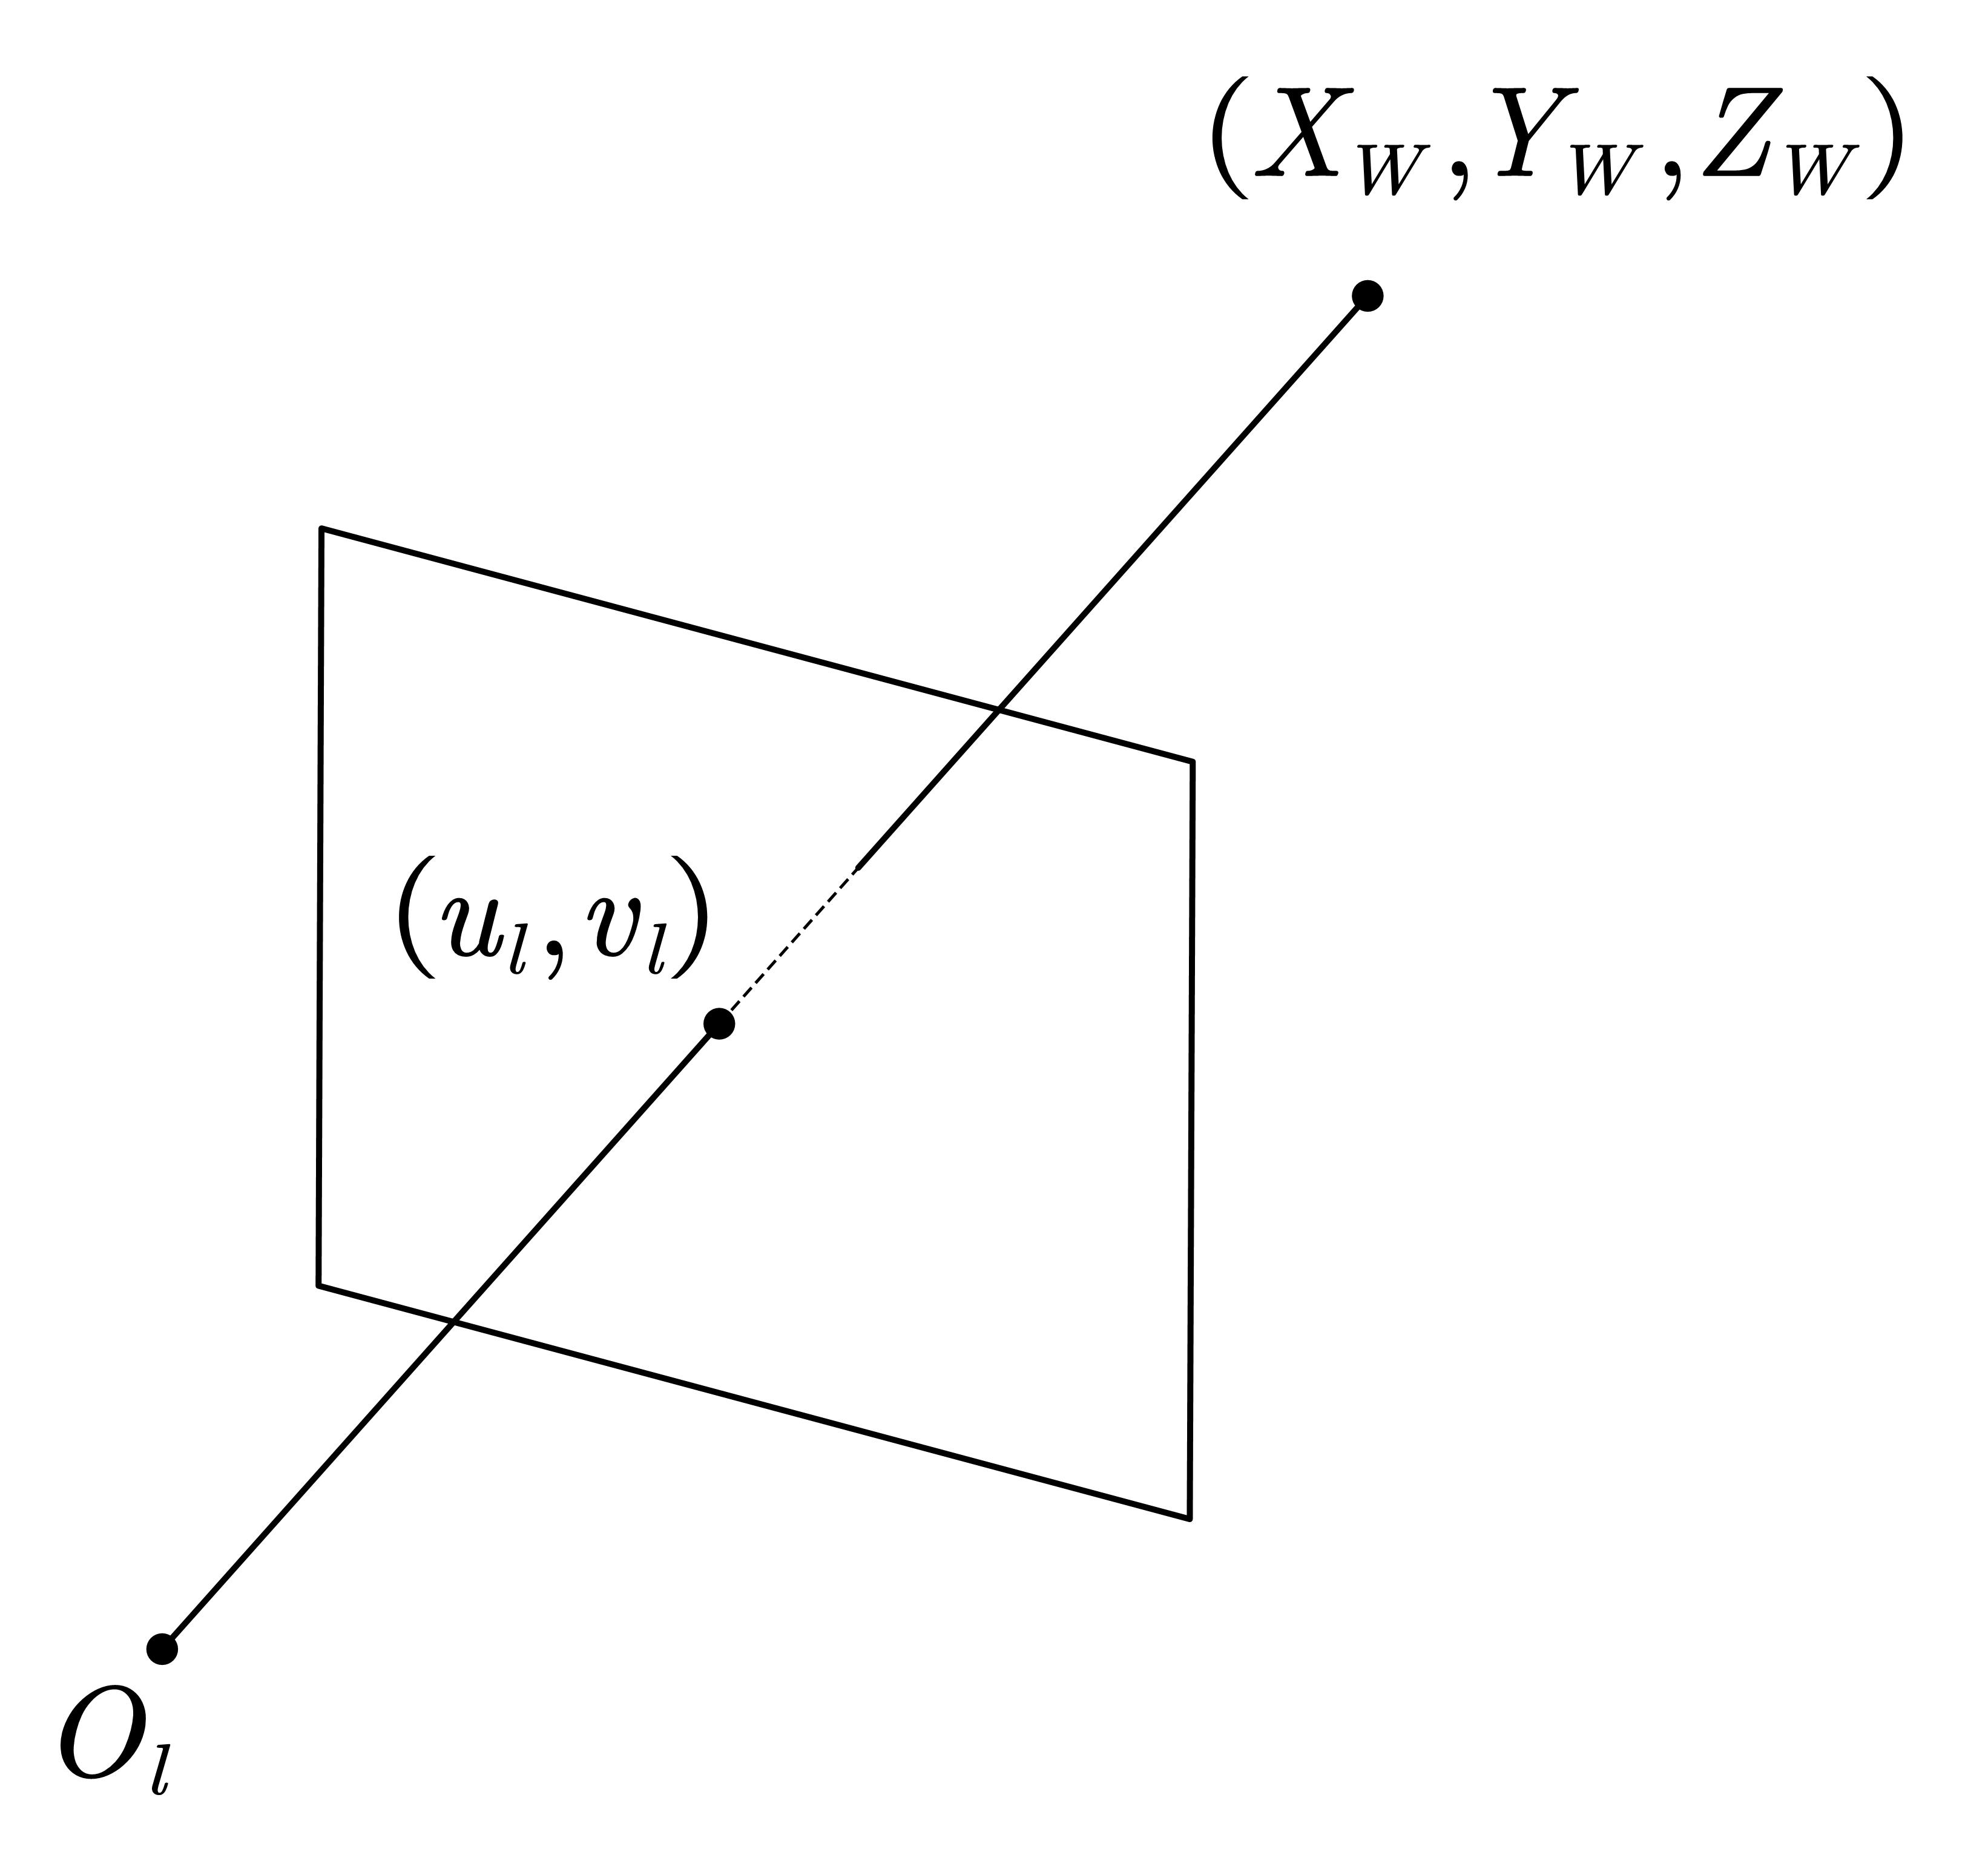
\includegraphics[scale=0.6]{单目相机参数求解}
			\end{center}
			\column{7.5cm}
			\begin{itemize}
				\item $O$是光圈中心
				\item $(u_l,v_l)$是像素点
				\item $(X_W,Y_W,Z_W)$是物体的坐标
			\end{itemize}
			\vspace{0.8em}
			\begin{equation}
				\begin{aligned}
					\left[ \begin{array}{c}
						u_l\\
						v_l\\
						1\\
					\end{array} \right] =\frac{1}{Z_C}\cdot K\cdot \left[ \begin{matrix}
						R&		T\\
					\end{matrix} \right] \cdot \left[ {\color{blue} \begin{array}{c}
							X_W\\
							Y_W\\
							Z_W\\
					\end{array}} \right] 
				\end{aligned}
			\end{equation}
		\end{columns}
	\end{frame}
	
	\begin{frame}
		\frametitle{如何得到$X_W,Y_W,Z_W$?}
		\begin{figure}
			\begin{center}
				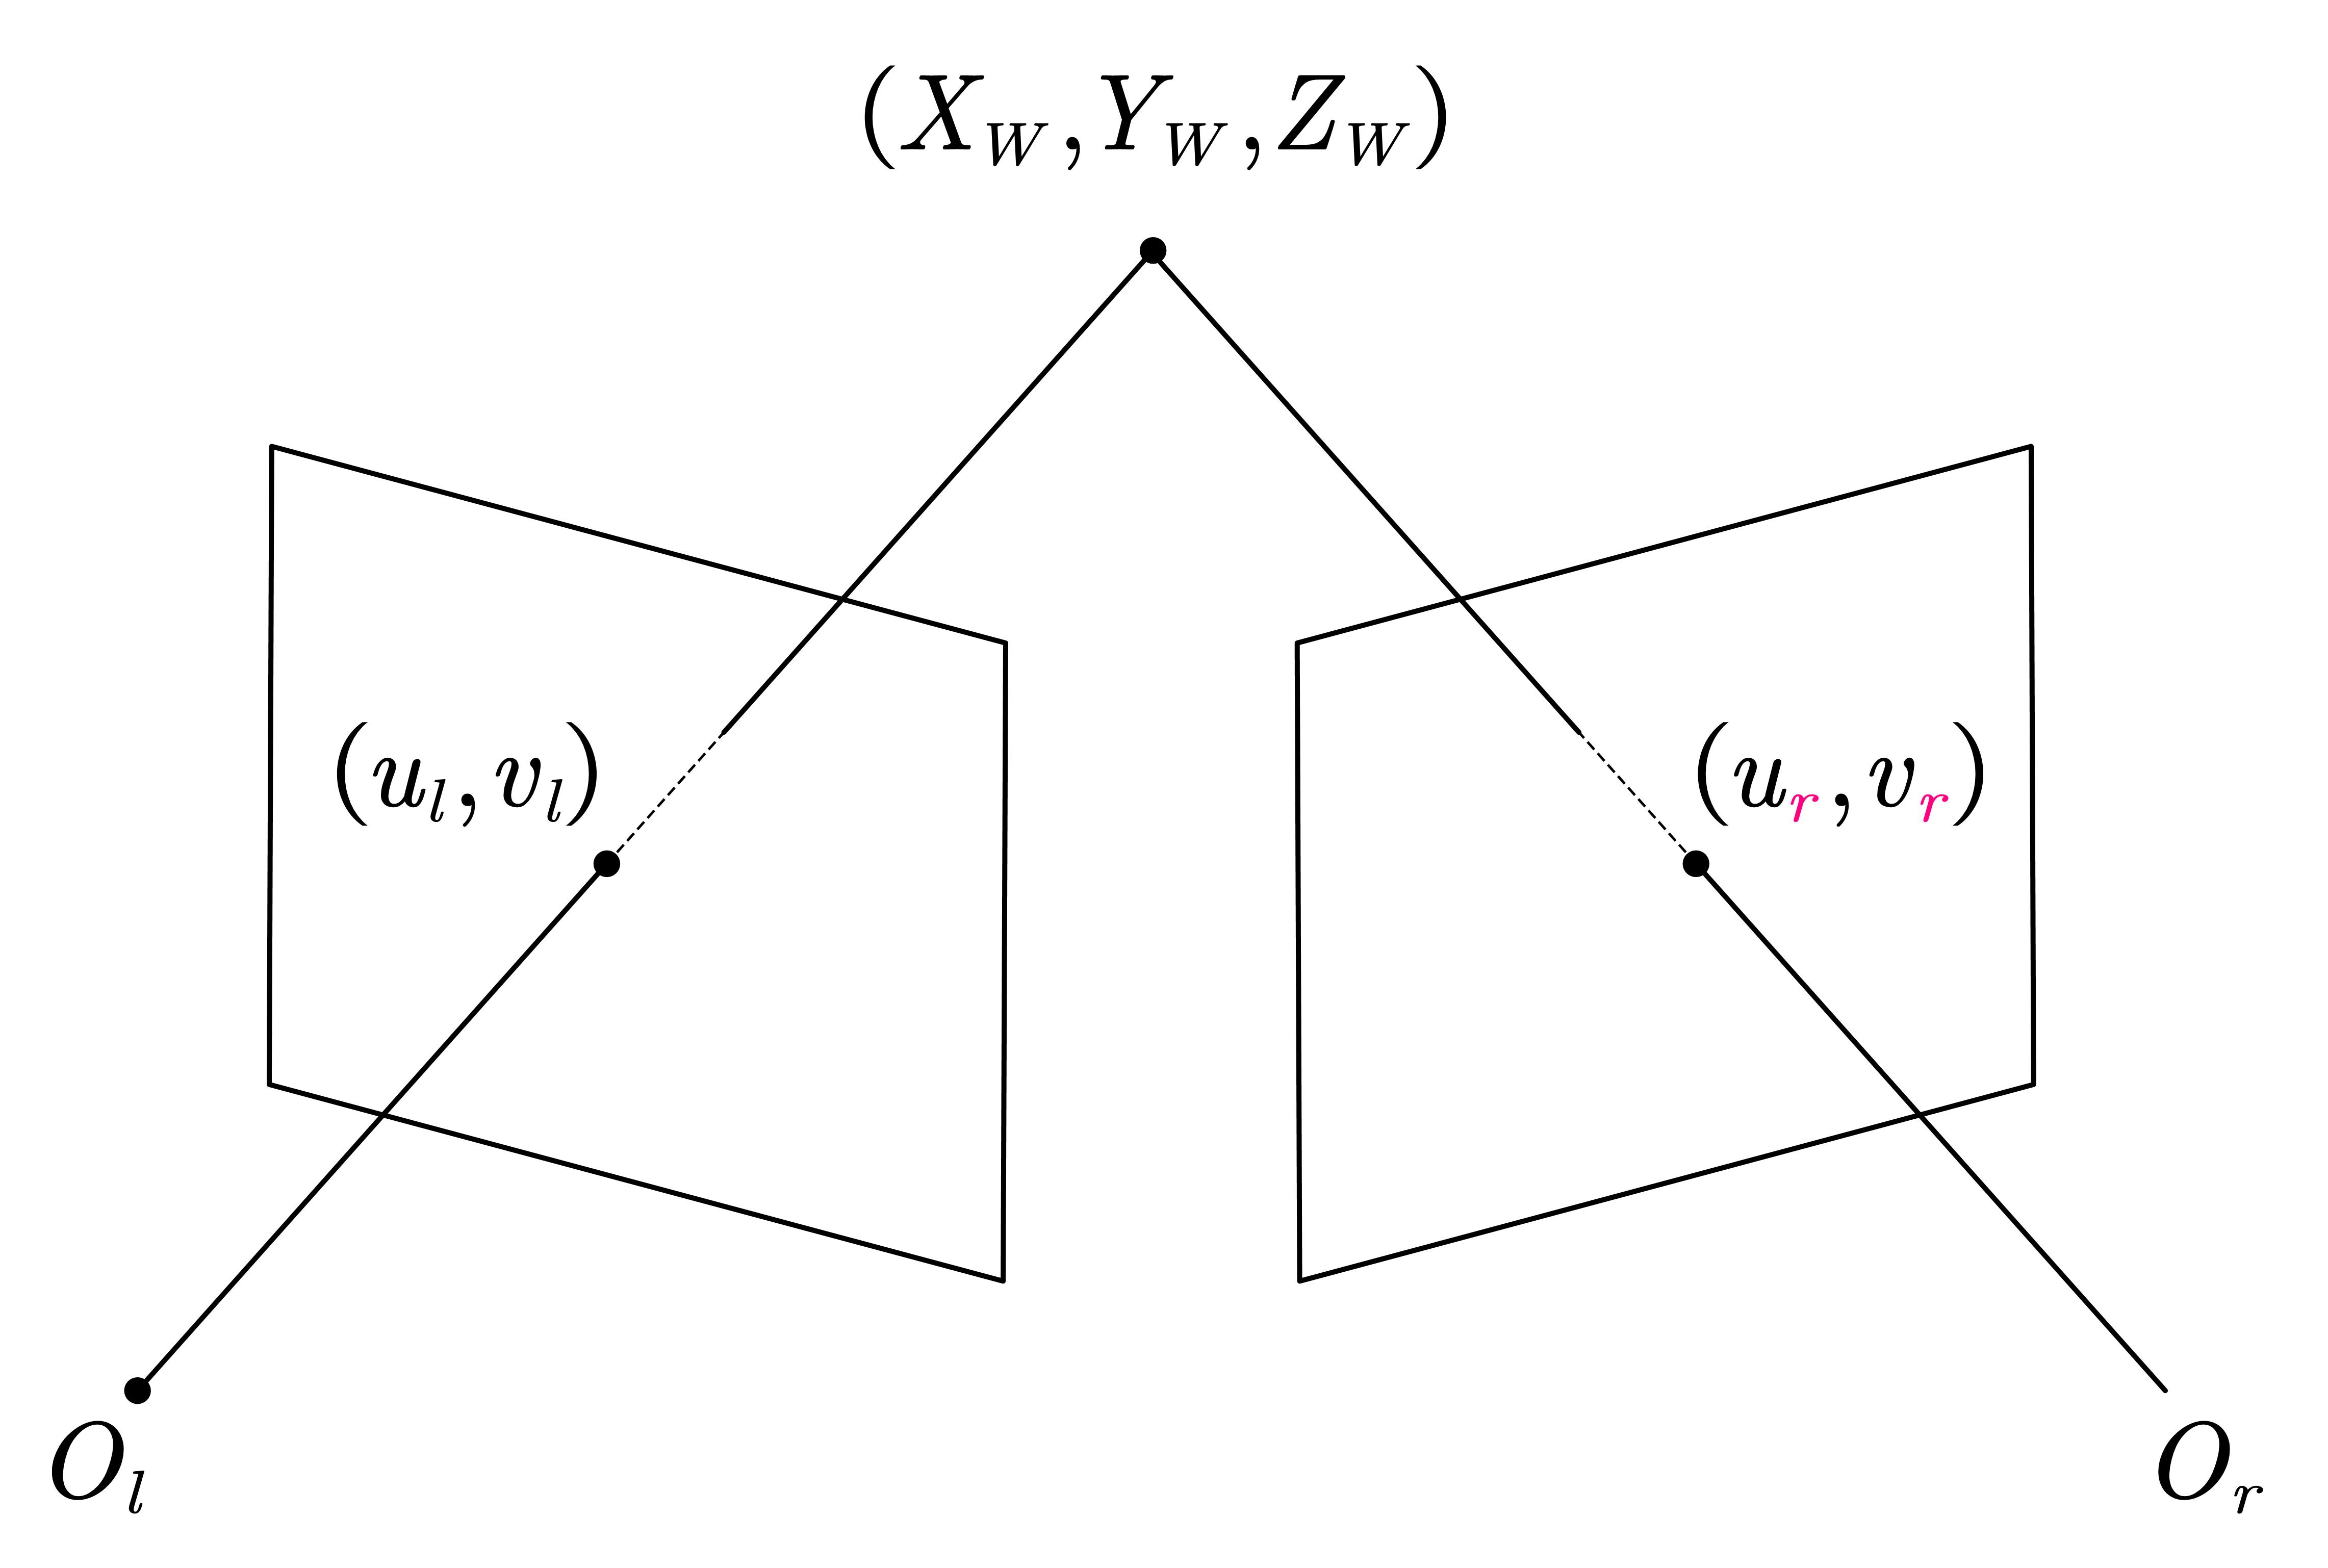
\includegraphics[scale=0.47]{单目相机参数求解-两个相机拍摄}
			\end{center}
		\end{figure}
		\begin{small}
			\begin{equation}
				\begin{aligned}
\begin{cases}
	\left[ \begin{array}{c}
		u_l\\
		v_l\\
		1\\
	\end{array} \right] =\frac{1}{Z_C}\cdot K\cdot \left[ {\color[RGB]{0, 128, 255} \begin{matrix}
			{\color{blue} R_l}&		{\color{blue} T_l}\\
	\end{matrix}} \right] \cdot \left[ \begin{array}{c}
		X_W\\
		Y_W\\
		Z_W\\
	\end{array} \right]\\
	\left[ \begin{array}{c}
		u_r\\
		v_r\\
		1\\
	\end{array} \right] =\frac{1}{Z_C}\cdot K\cdot \left[ {\color[RGB]{0, 128, 255} \begin{matrix}
			{\color[RGB]{0, 0, 240} R_r}&		{\color[RGB]{0, 0, 240} T_r}\\
	\end{matrix}} \right] \cdot \left[ \begin{array}{c}
		X_W\\
		Y_W\\
		Z_W\\
	\end{array} \right]\\
\end{cases}
				\end{aligned}
			\end{equation}
		\end{small}
		
	\end{frame}	
	
	
	\begin{frame}
		\frametitle{左右相机之间的位姿关系}
		\begin{block}{求解过程}
			\begin{itemize}
				\item 分别按单目相机确定内外参,得到$R_1,R_2,T_1,T_2$
				\item 对任意点$P_W=(X_W,Y_W,Z_W)$,在左右相机坐标系下的坐标分别为$x_{c1},x_{c2}$,且有以下关系(仅以$X_W$为例):
				\begin{align}
					\begin{cases}
						x_{c1}=R_1X_W+T_1\\ 
						x_{c2}=R_2X_W+T_2
					\end{cases}
				\end{align}
				\item 消去$X_W$,得到$x_{c1}={\color[RGB]{0, 0, 240} R_1{R{\color[RGB]{0, 0, 240} _2}}^{-1}}x_{c2}+{\color[RGB]{0, 0, 240} T_1-{R{\color[RGB]{0, 0, 240} _2}}^{-1}T_2}$,令:
				\begin{align}
					\begin{cases}
						R=R_1{R_2}^{-1}\\
						T=T_1-{R_2}^{-1}T_2
					\end{cases}
				\end{align}
			\end{itemize}
		\end{block}
	\end{frame}
	

	


		
		\begin{frame}
		\frametitle{极线约束\footnote{极线约束是一种原理,其过程称为极线校正}(Epipolar Constraint)}
		
		\begin{columns}
		\column{5cm}

		\begin{figure}
			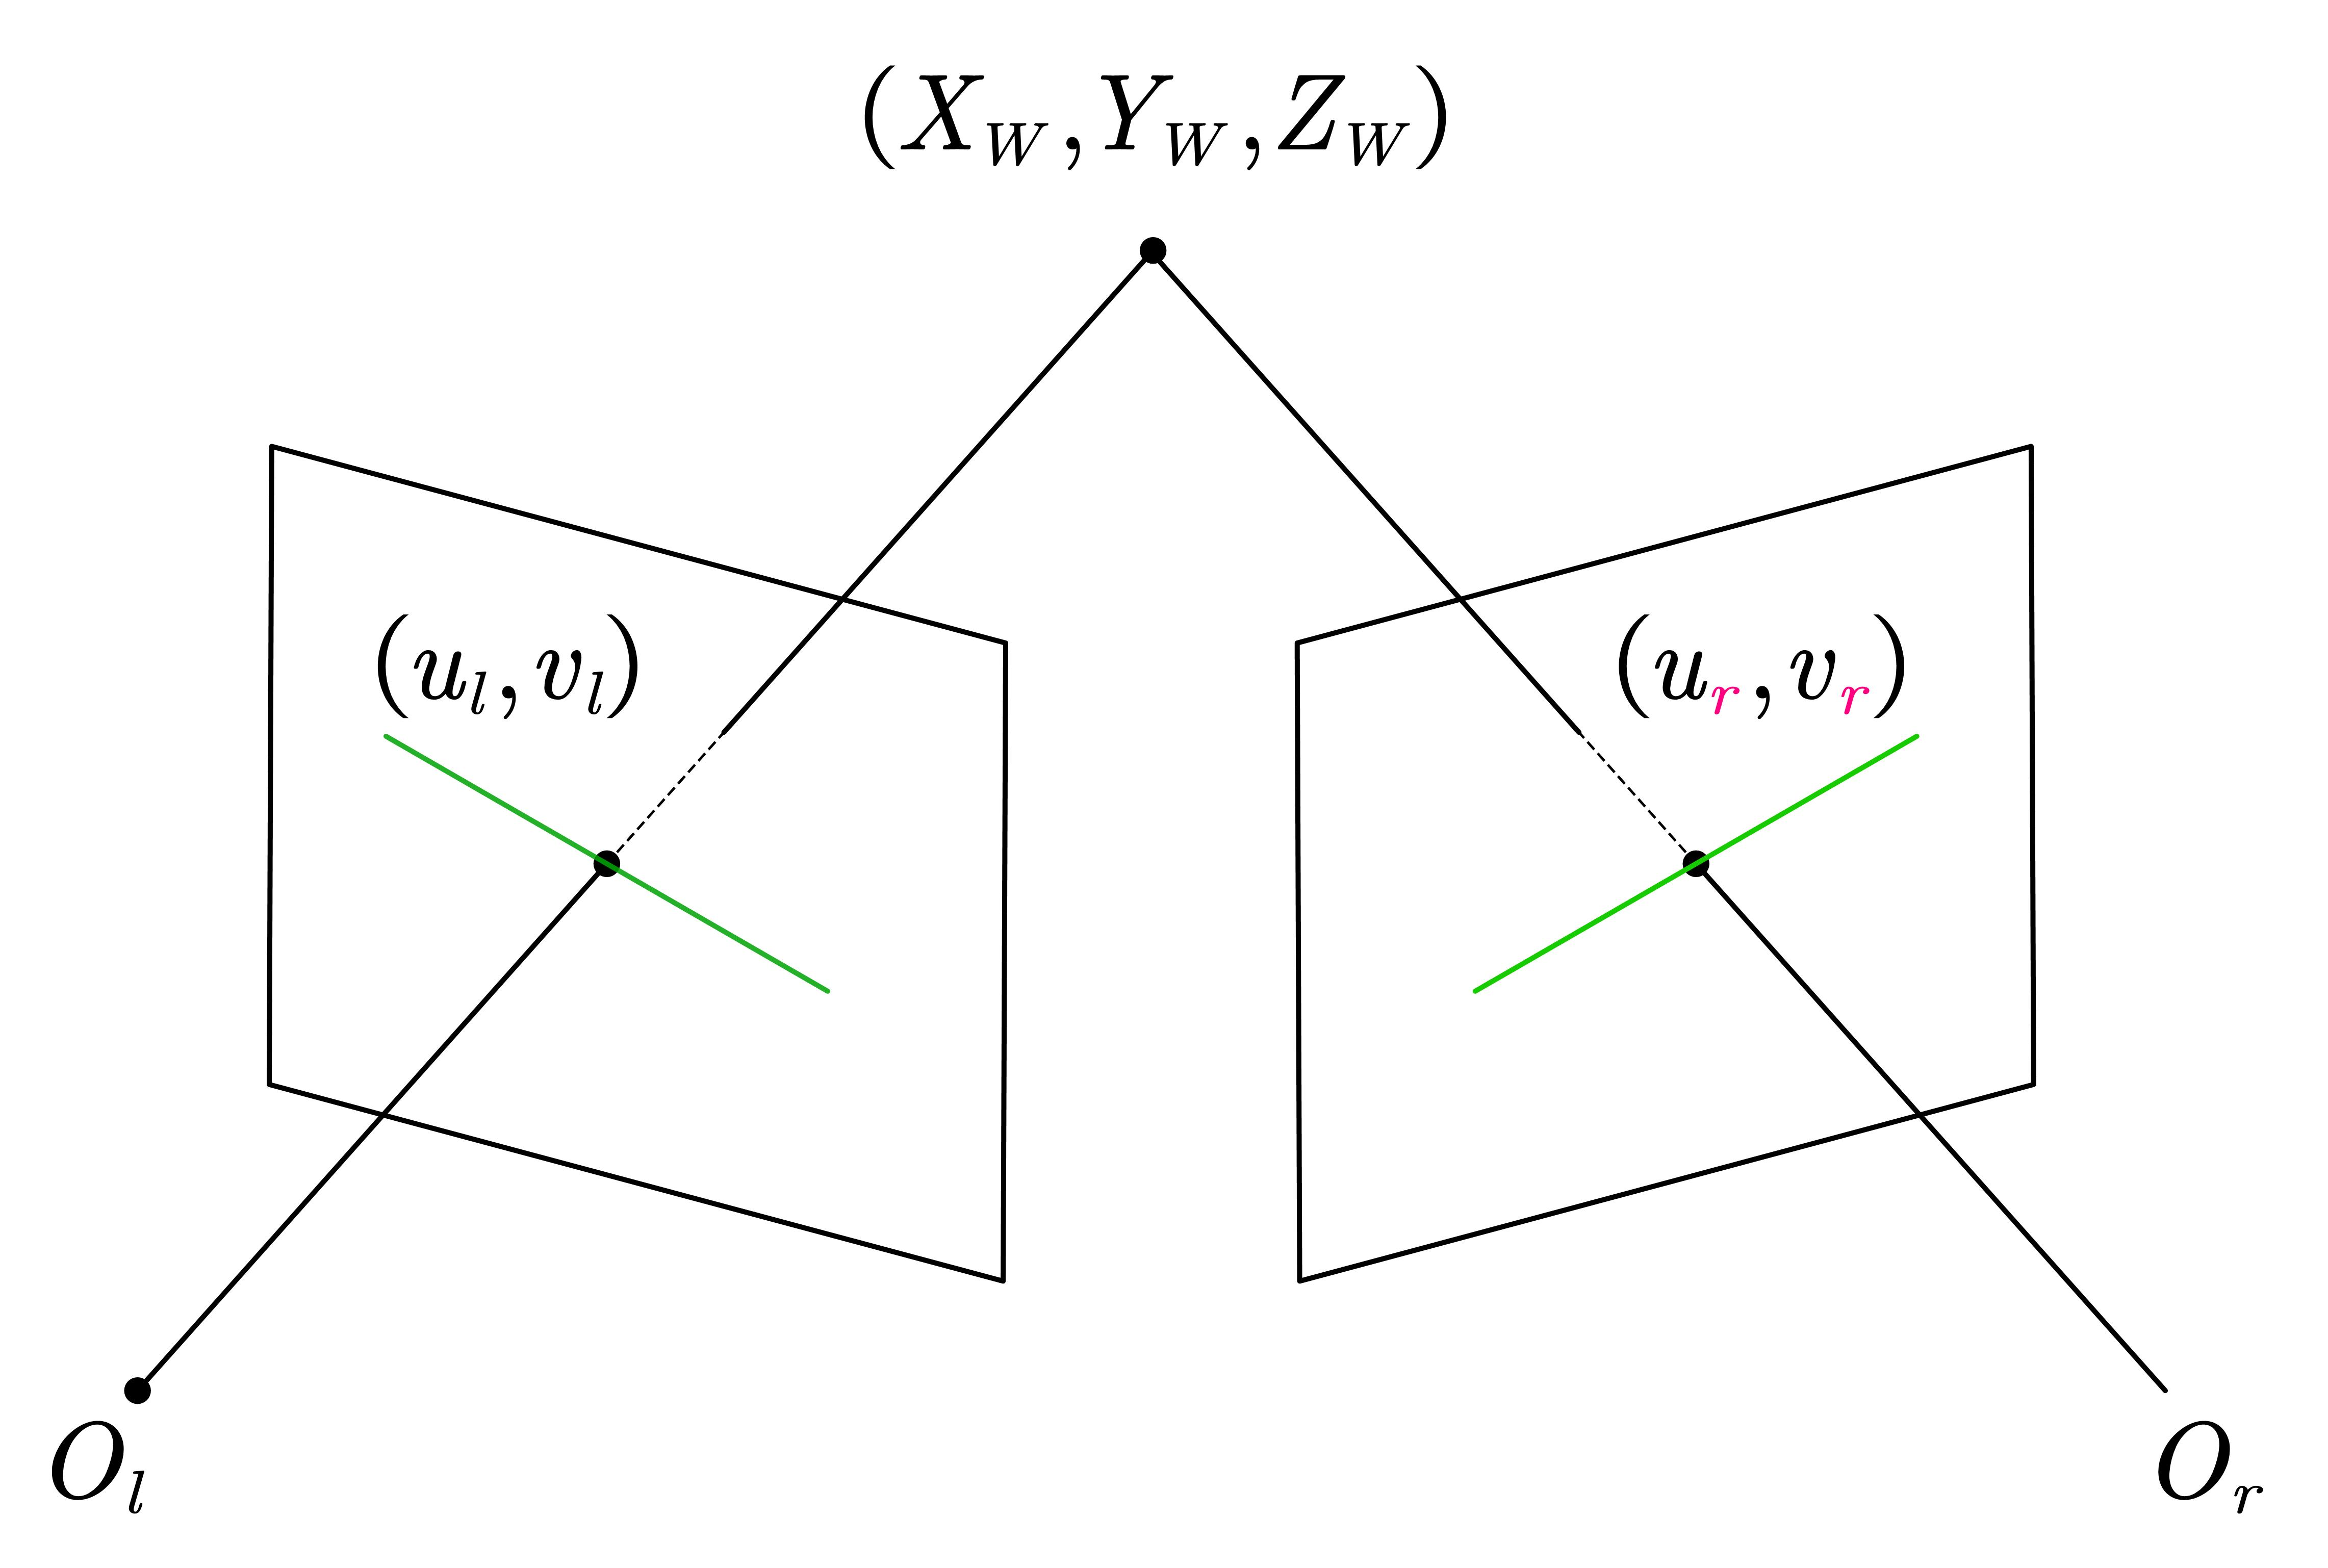
\includegraphics[scale=0.5]{双目相机-极线约束1}
		\end{figure}
		\column{6cm}

		\begin{figure}
			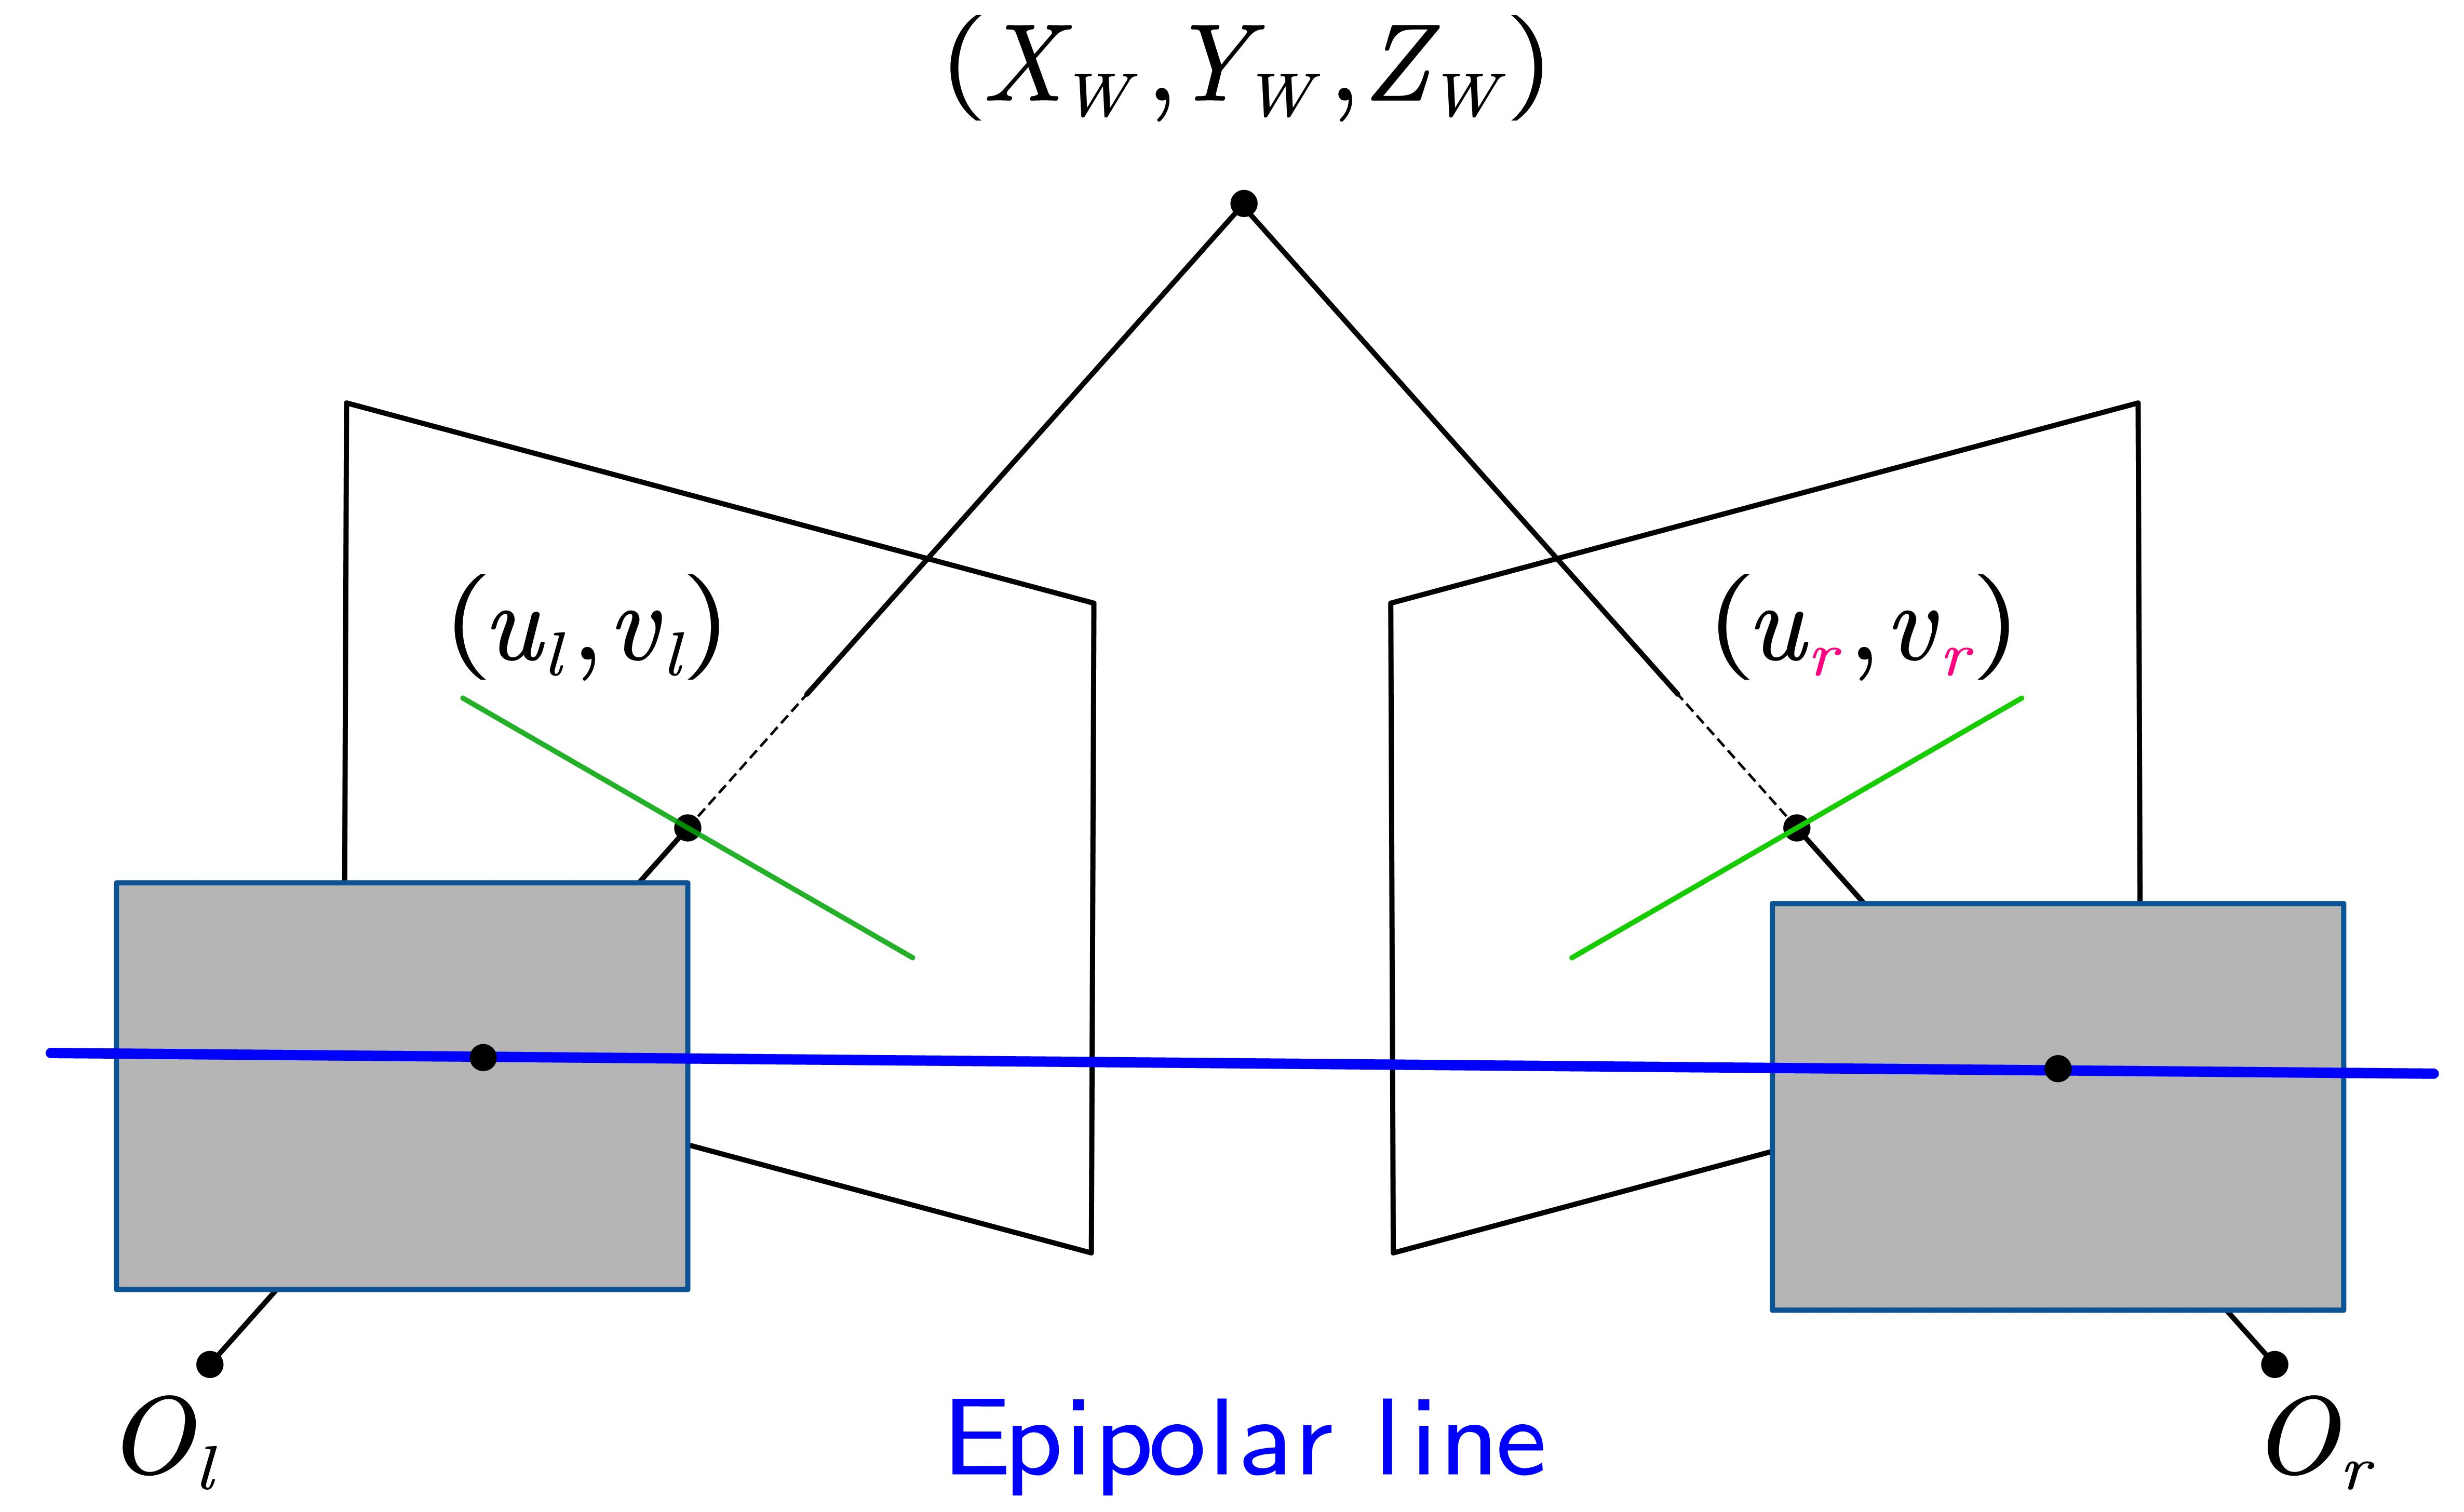
\includegraphics[scale=0.5]{双目相机-极线约束2}
		\end{figure}
		\end{columns}	
		\end{frame}
	
		\begin{frame}
		\frametitle{极线校正(Stereo Rectify)}
		\begin{columns}
		\column{5cm}
		\begin{center}
		\begin{itemize}
			\item 像平面平行
		\end{itemize}
		\end{center}
		\begin{figure}
			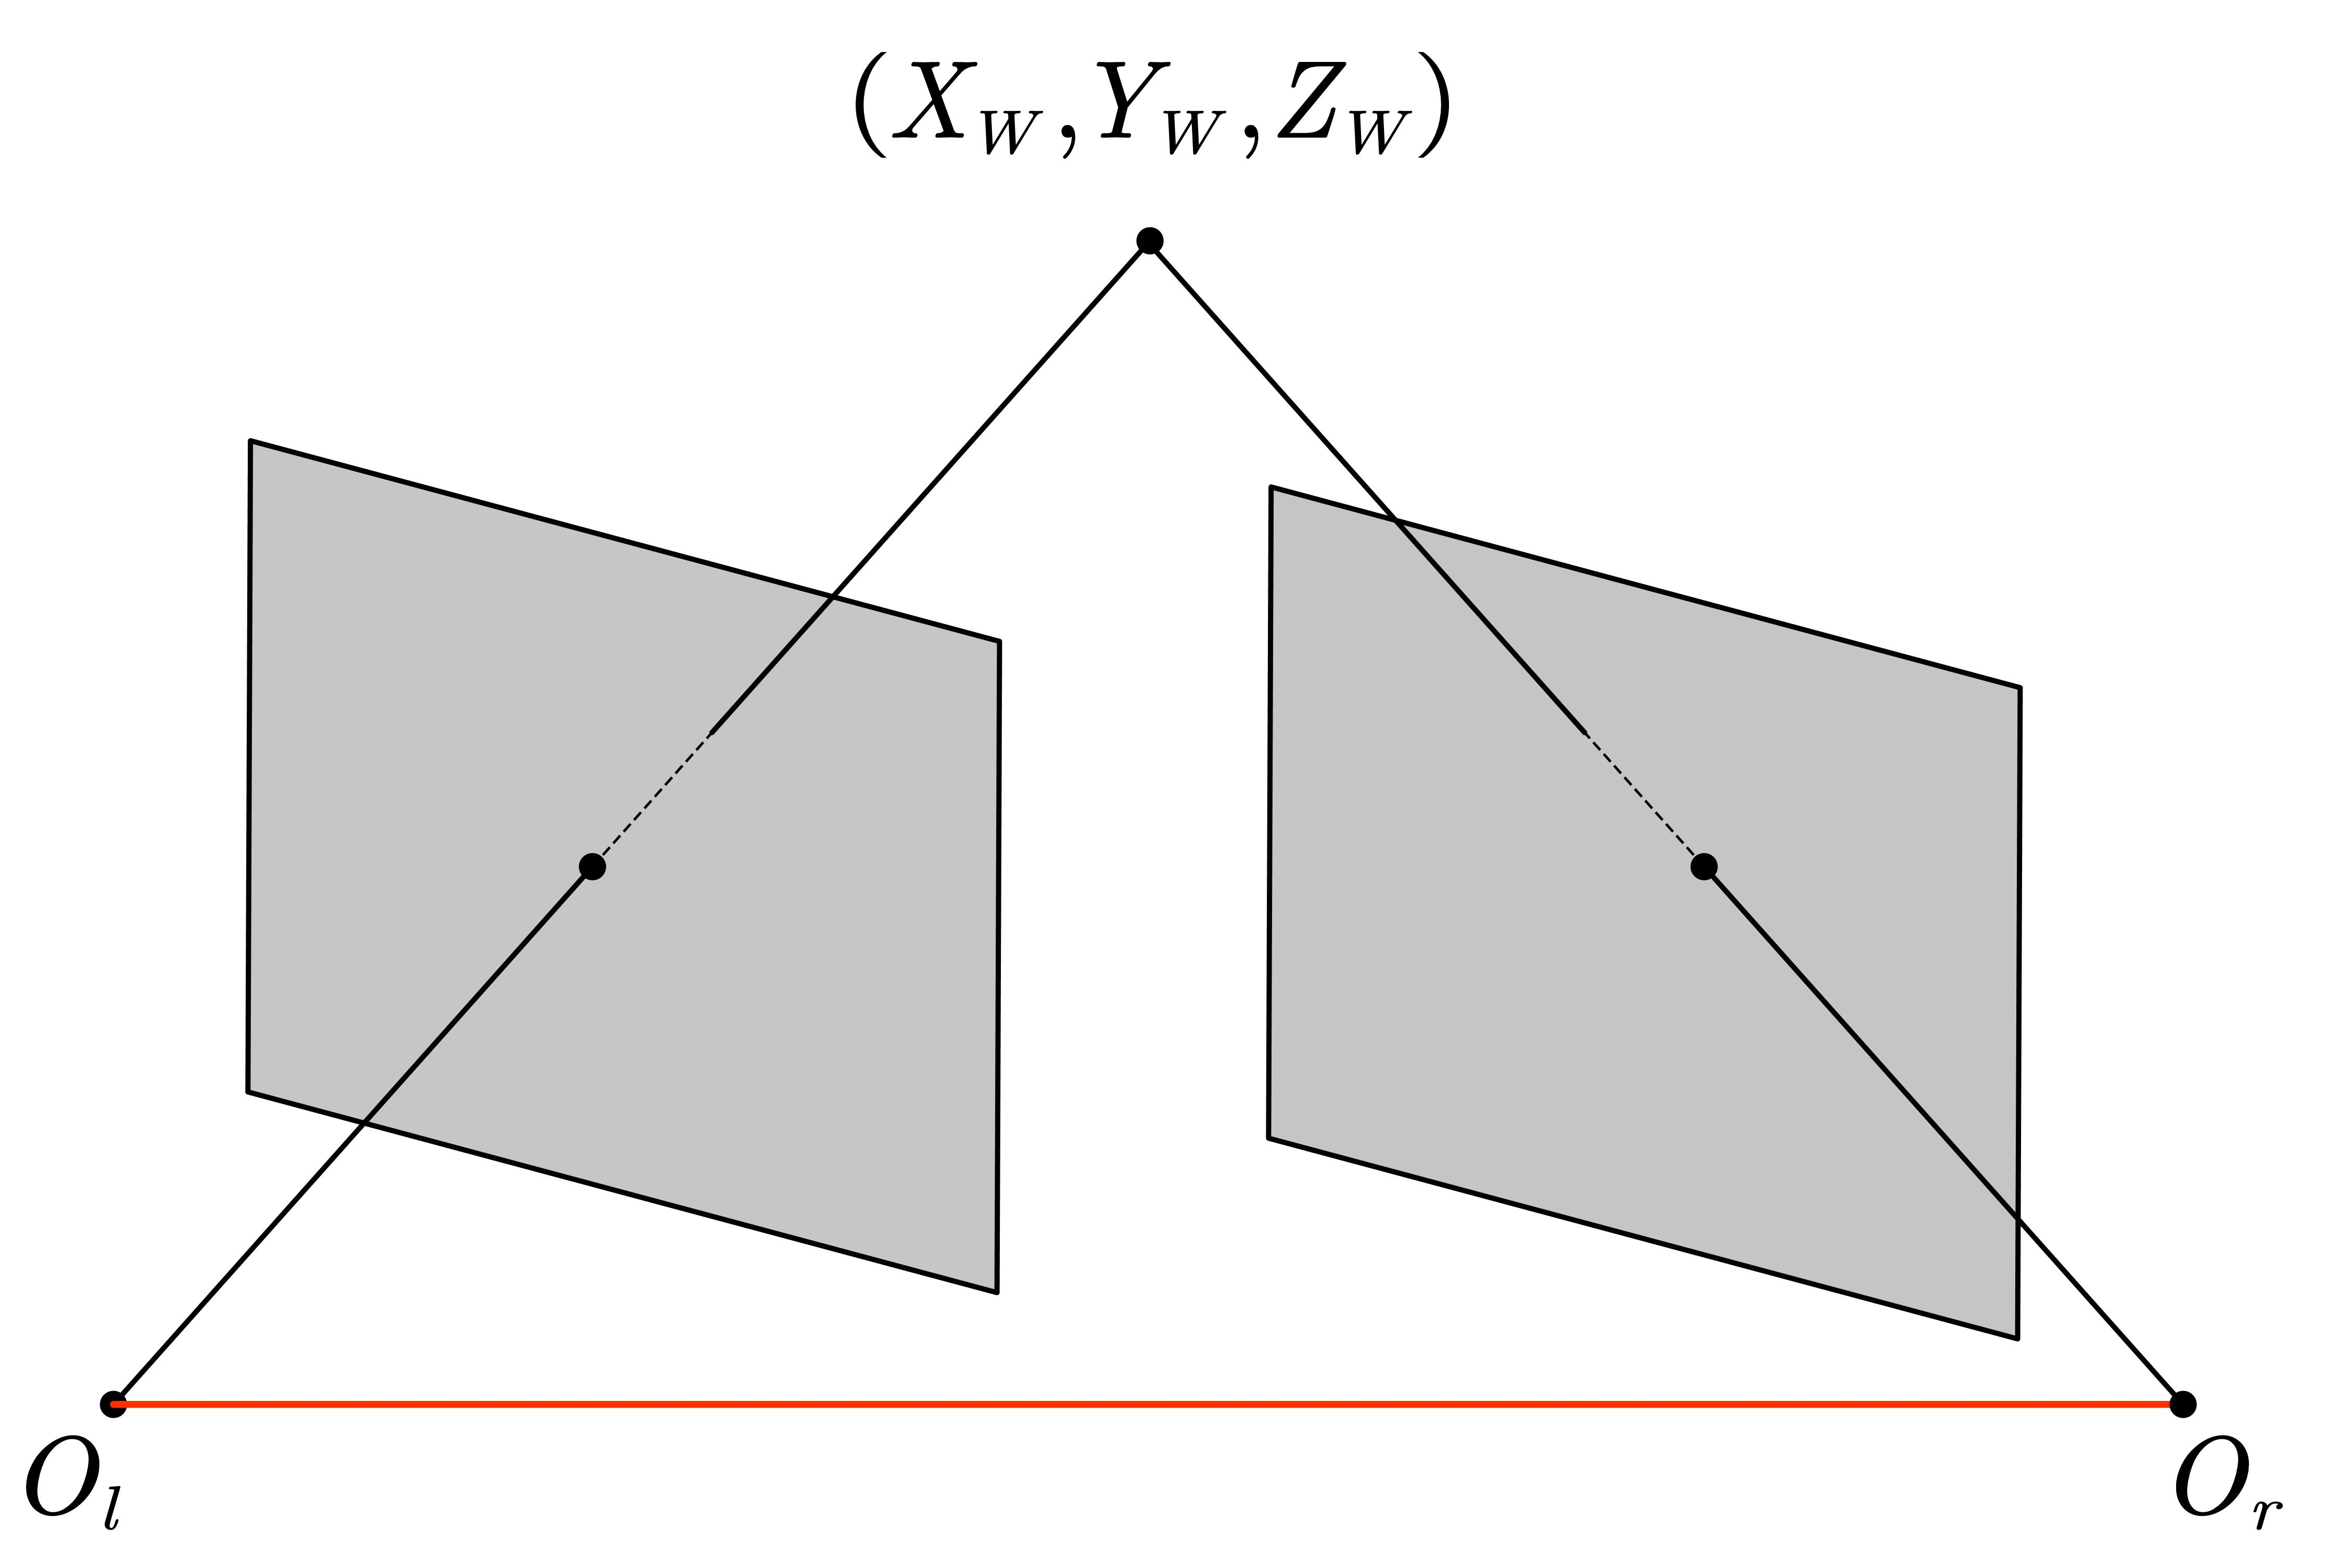
\includegraphics[scale=0.45]{极线校正-像平面平行}
		\end{figure}	
		\column{5cm}
		\begin{center}
		\begin{itemize}
			\item 行对准
		\end{itemize}
		\end{center}
		\begin{figure}
			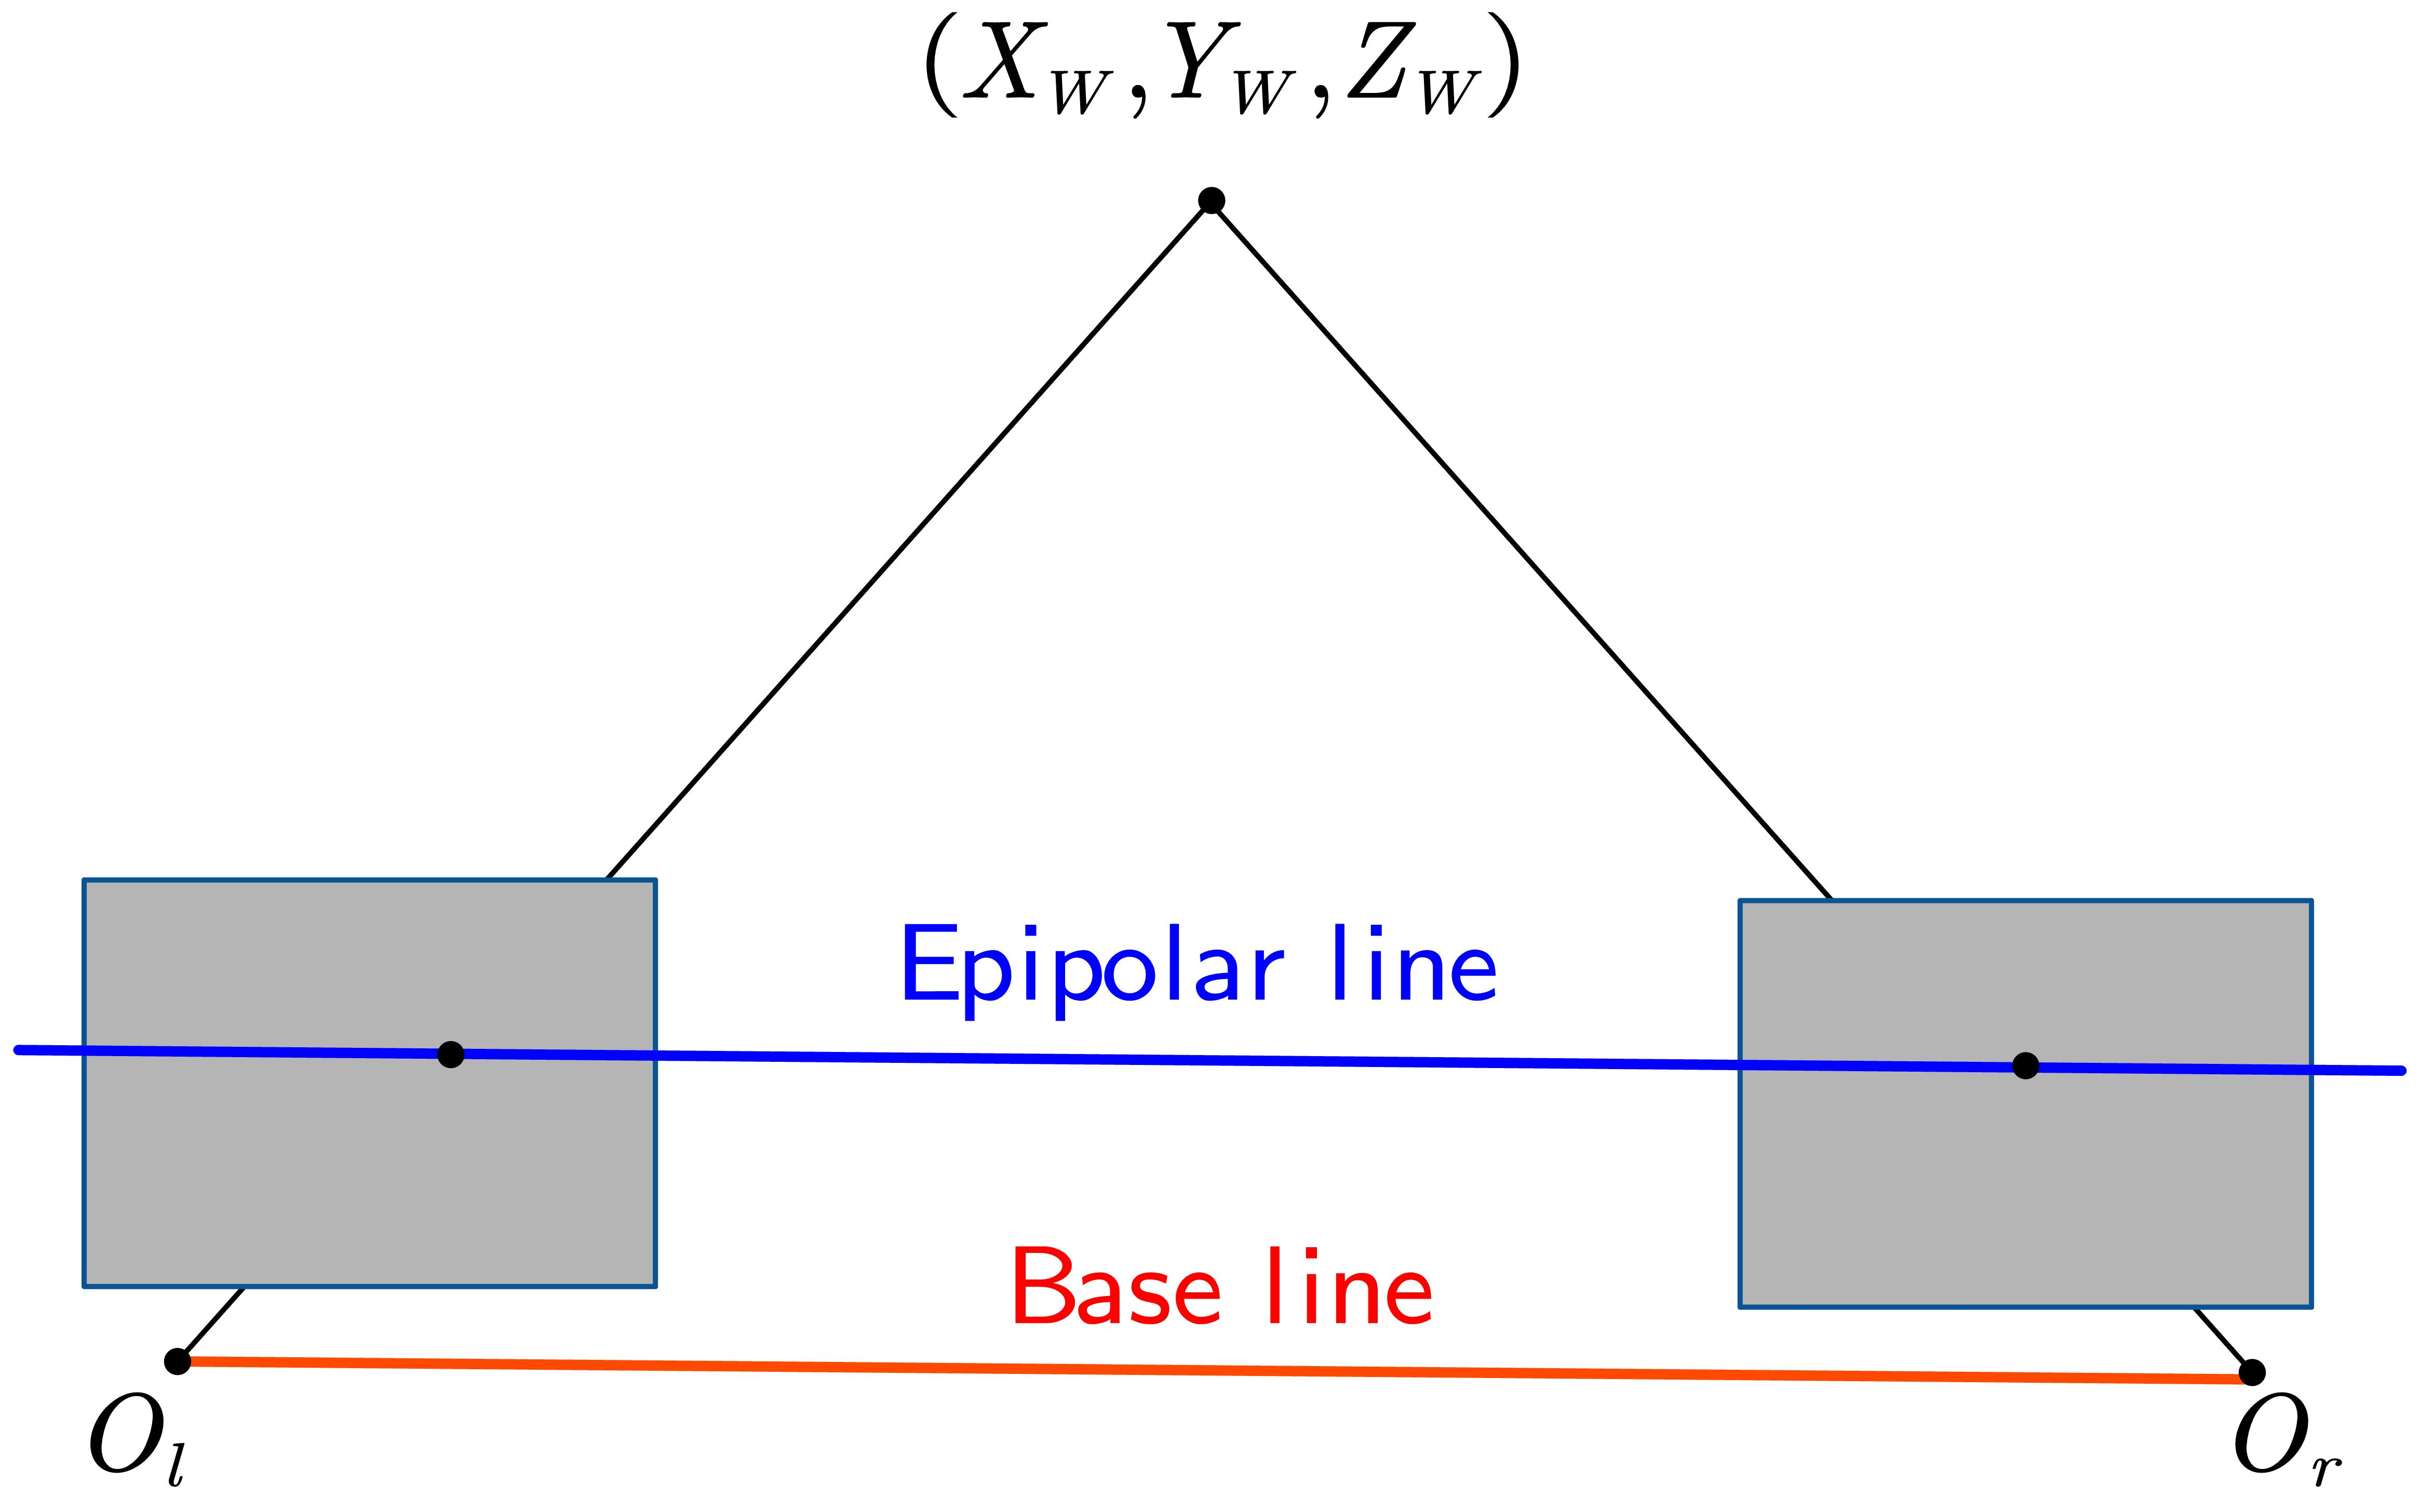
\includegraphics[scale=0.47]{极线校正-行对准}
		\end{figure}
		\end{columns}
		\end{frame}
	
		\begin{frame}
		\frametitle{极线校正-像平面平行}
		\begin{columns}
		\column{5cm}
		\begin{figure}
		\begin{center}
			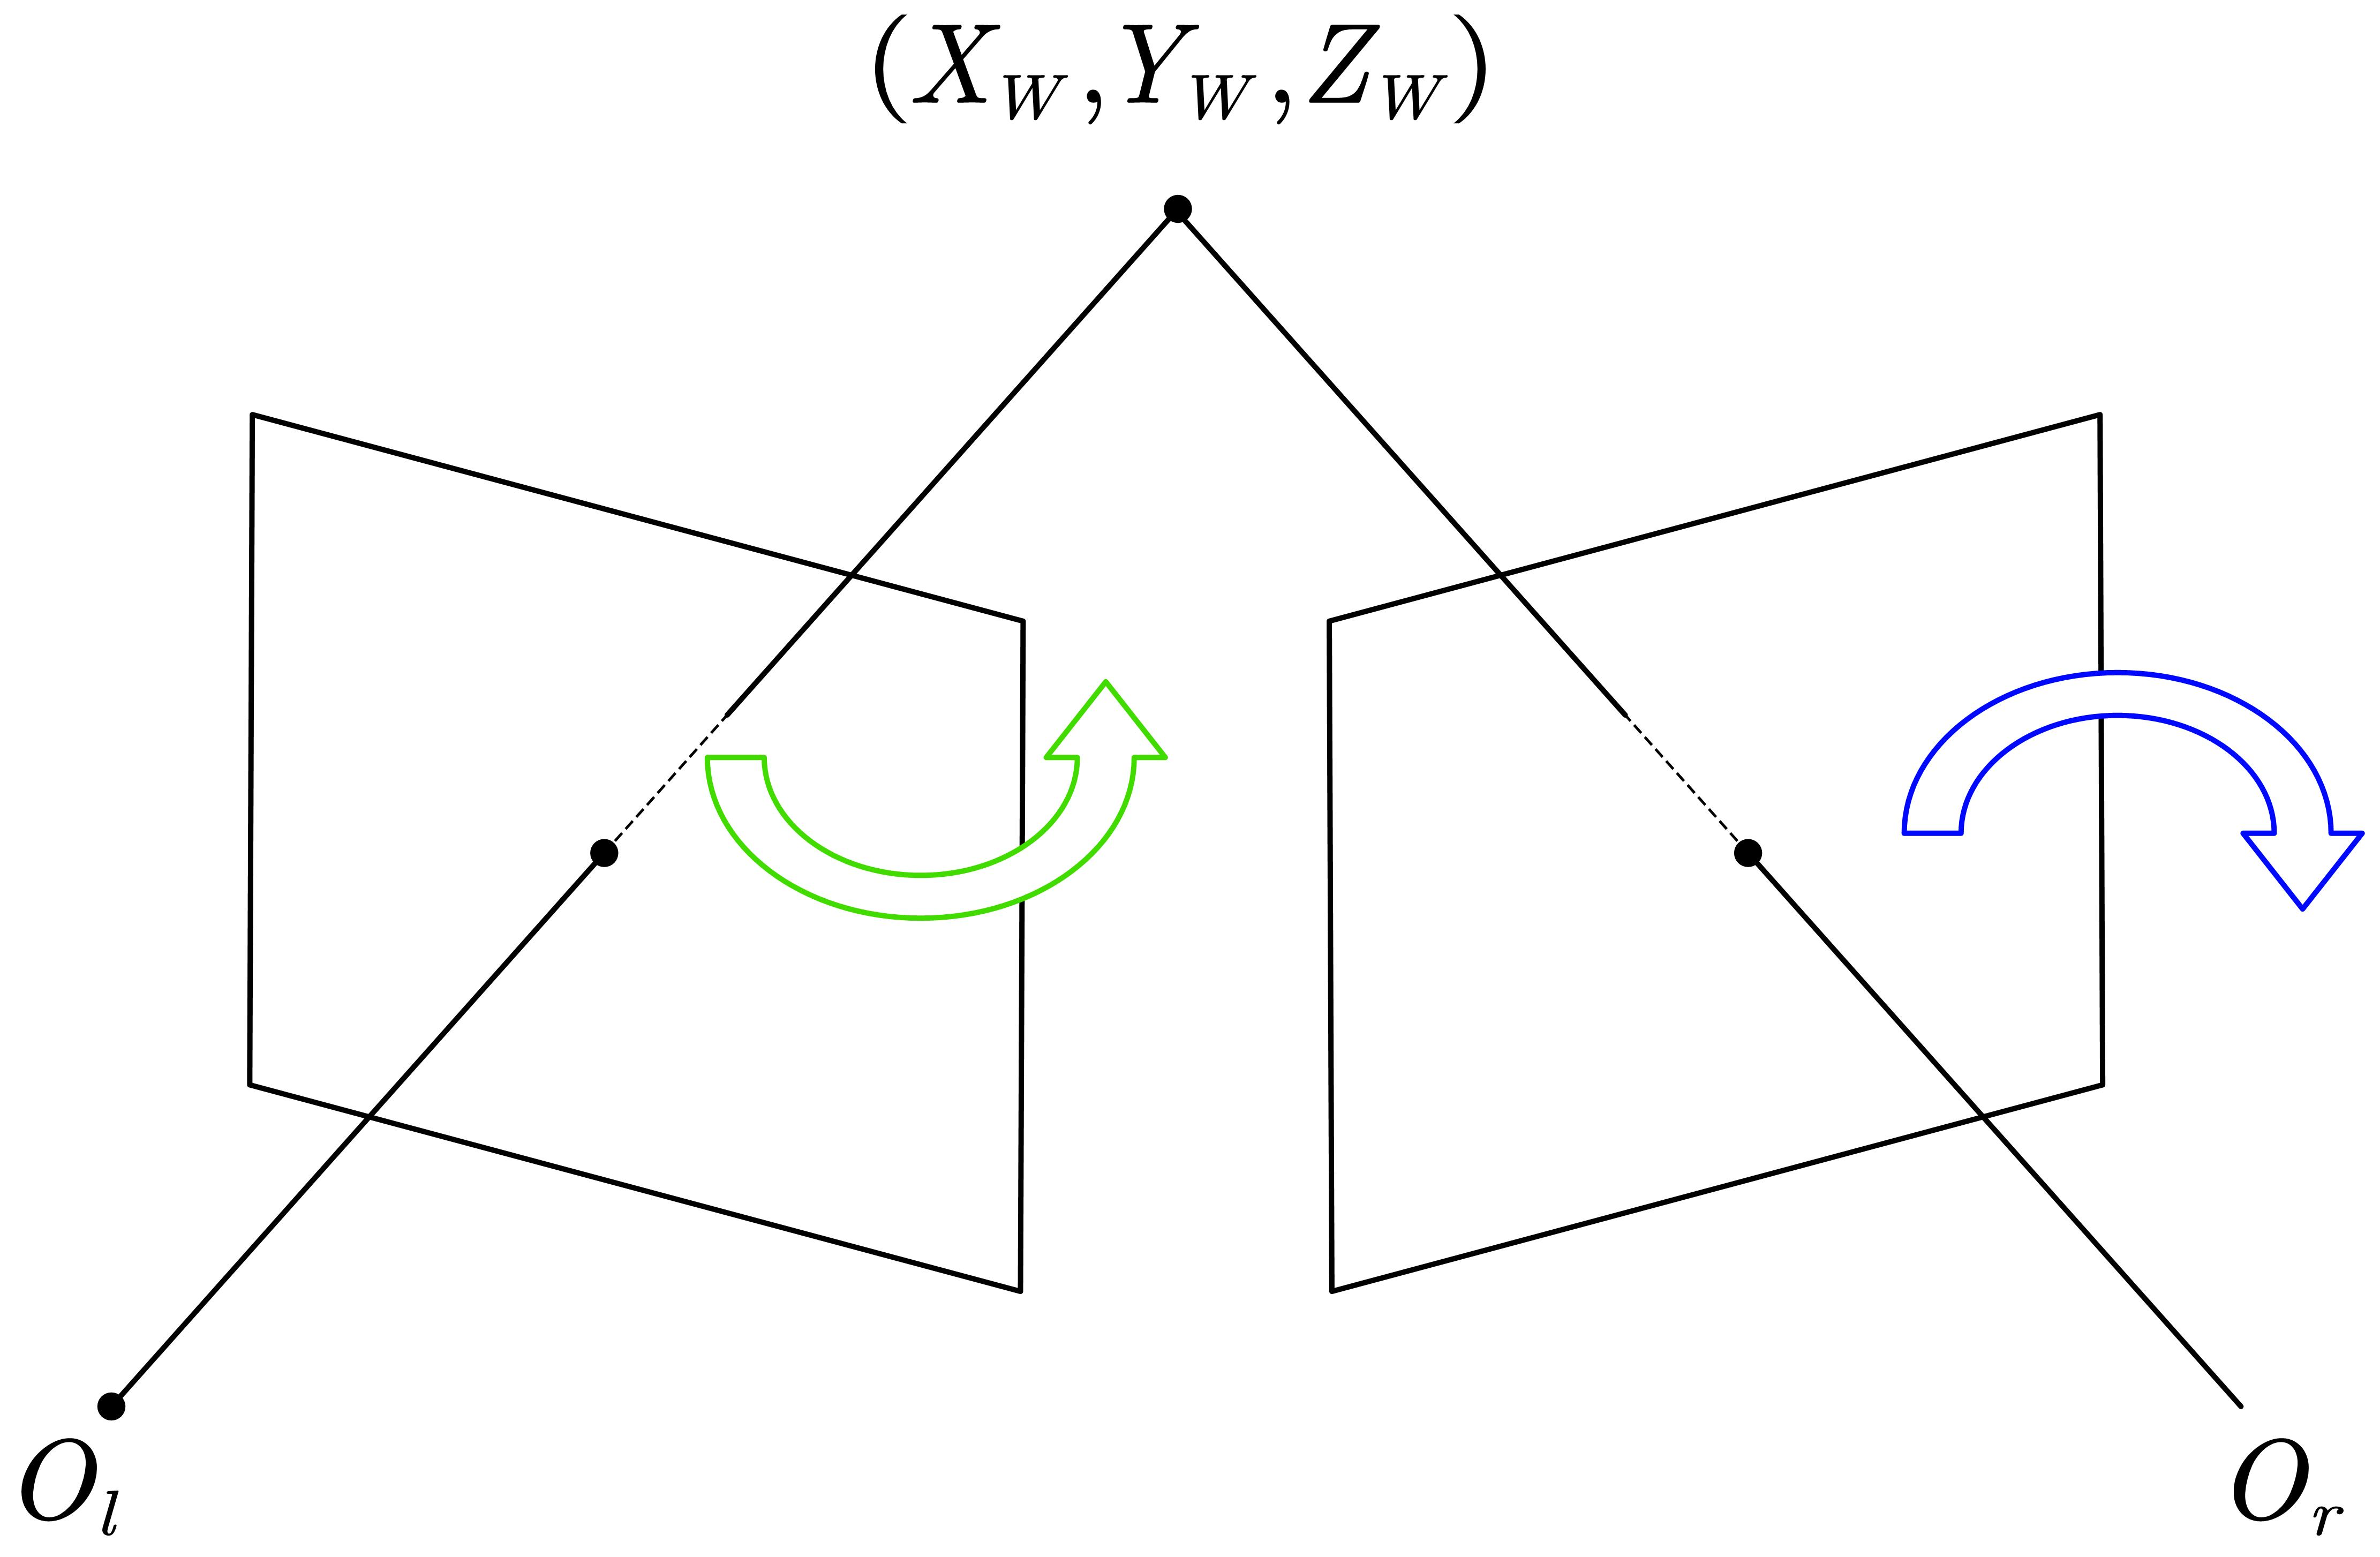
\includegraphics[scale=0.5]{极线校正-像平面平行-旋转}
		\end{center}
		\end{figure}
		\column{5cm}
		\begin{itemize}
			\item 左右像平面各旋转一半
			\item $r_l=R^{\frac{1}{2}},r_r=R^{-\frac{1}{2}}$			
		\end{itemize}
		\end{columns}
		\end{frame}
	
		\begin{frame}
		\frametitle{极线校正-行对准}
		\begin{columns}
		\column{5cm}
		\begin{figure}
		\begin{center}
				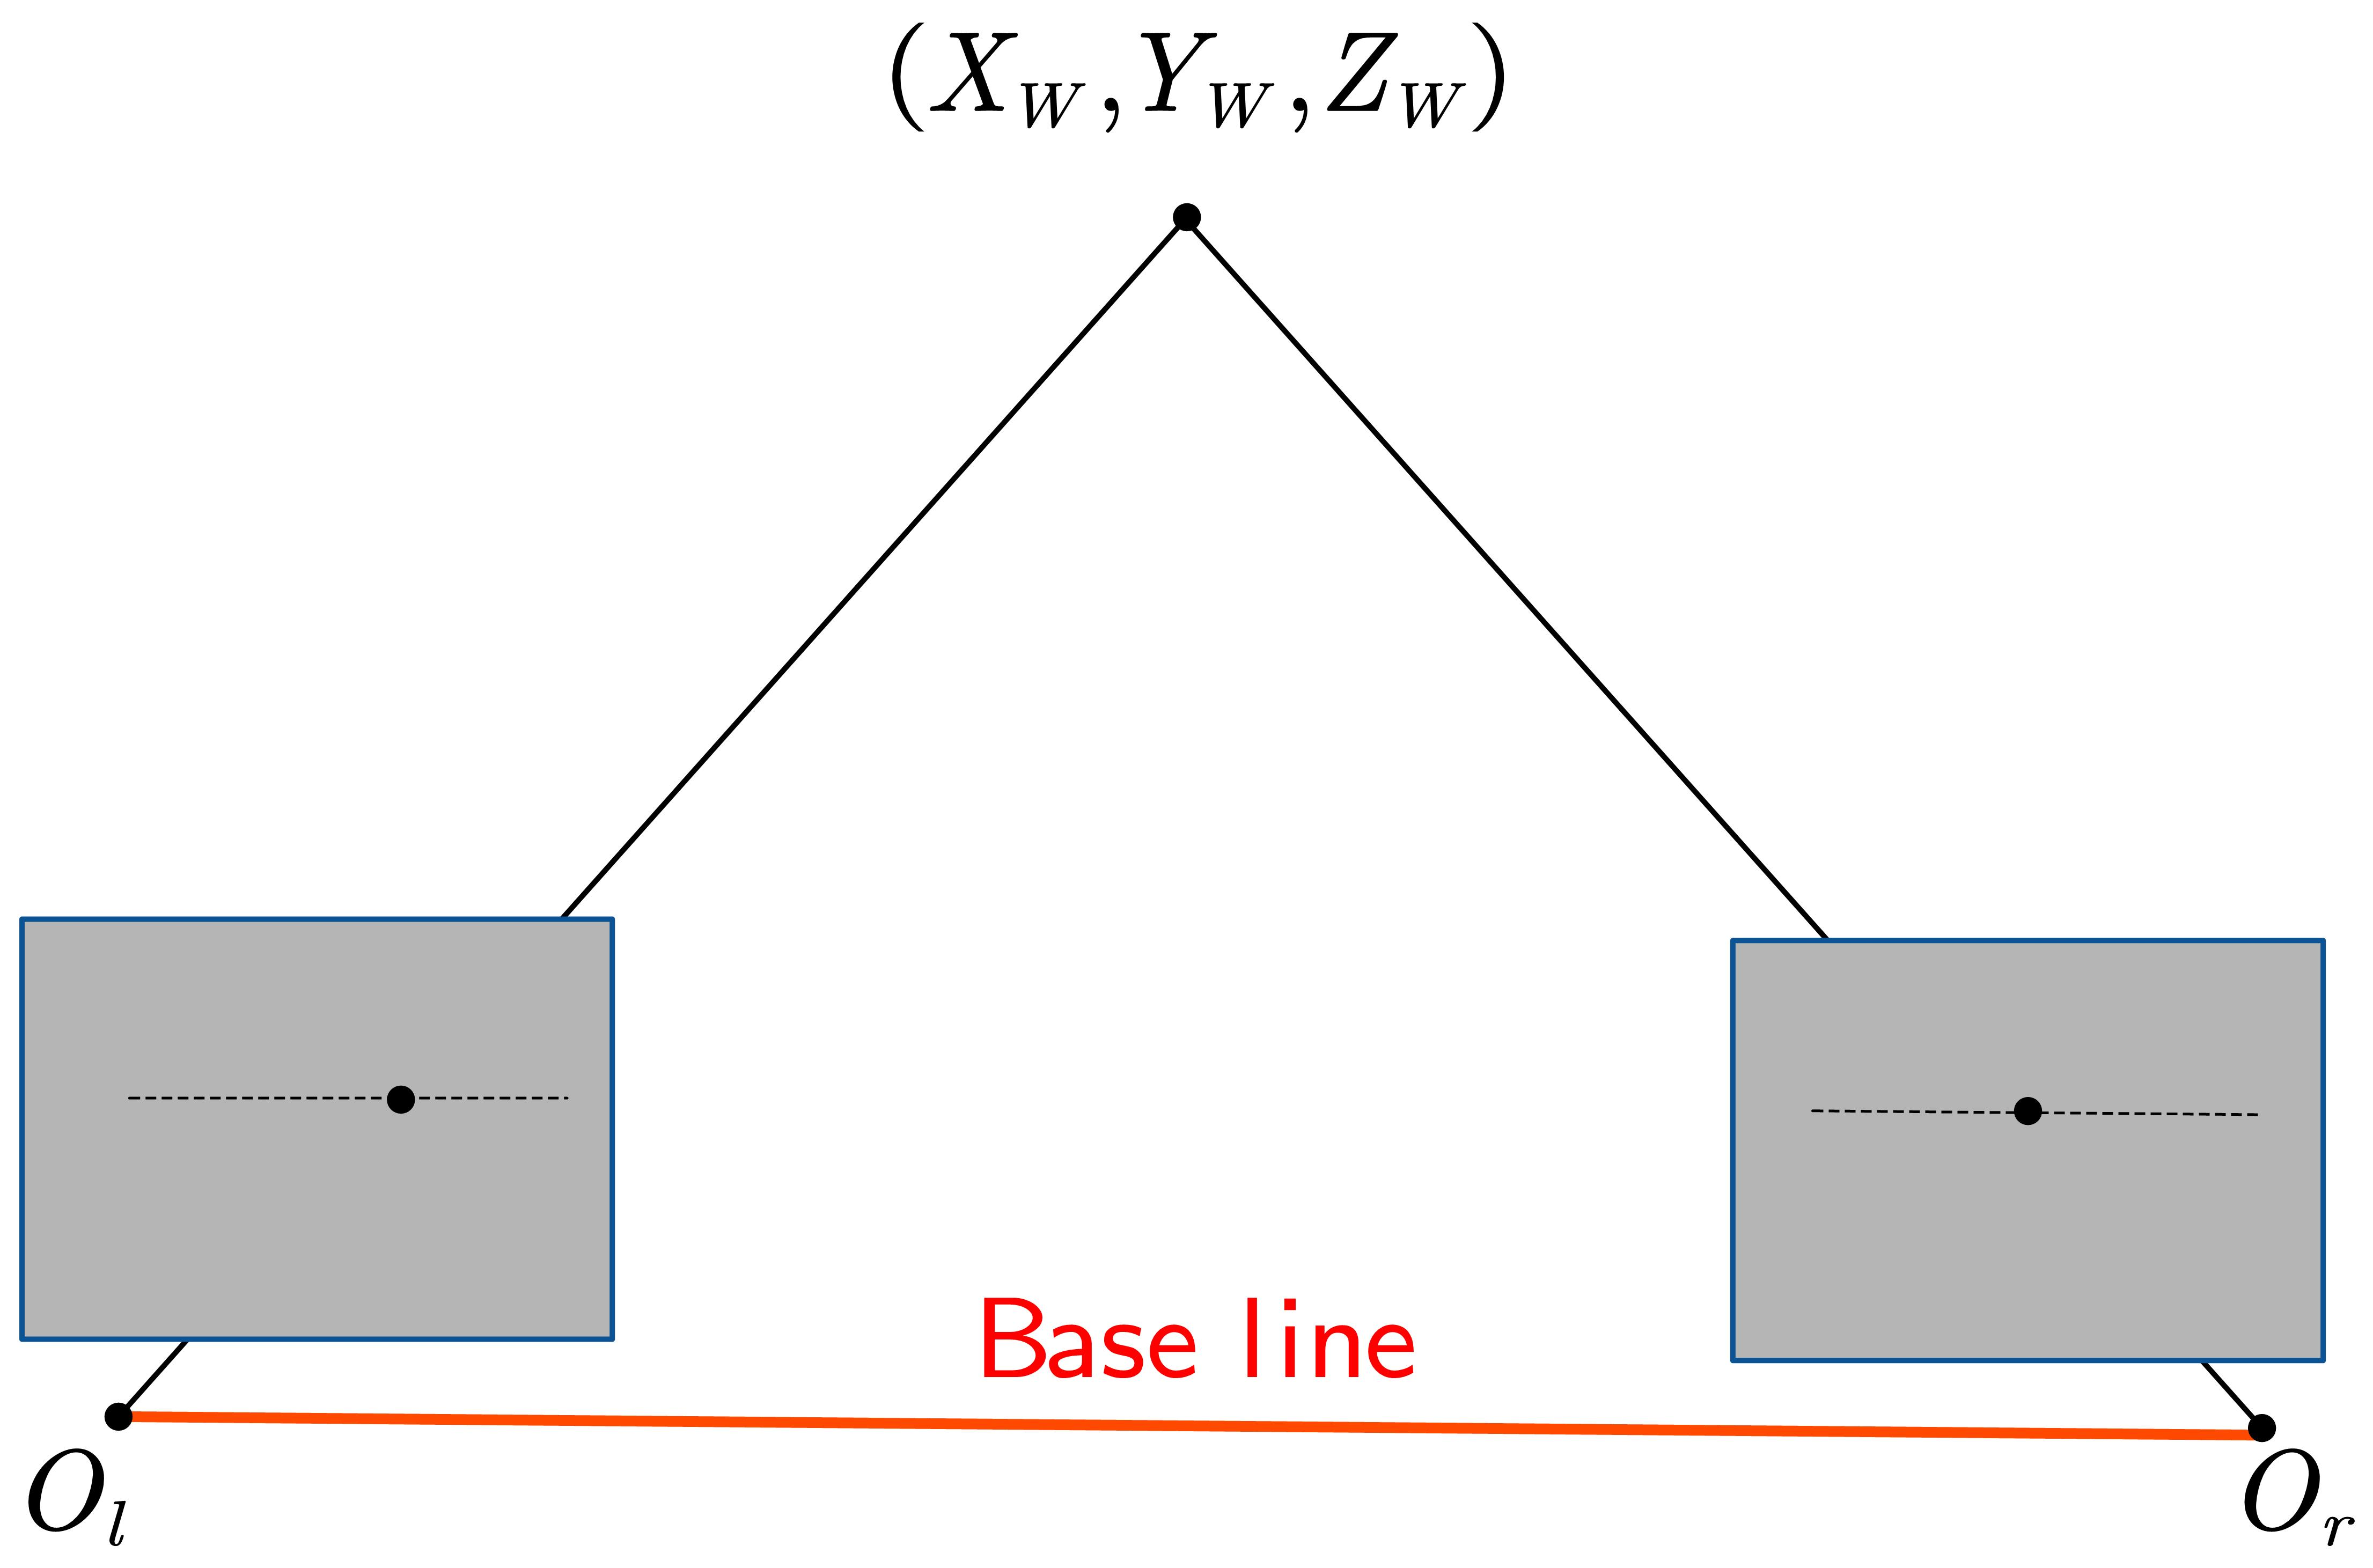
\includegraphics[scale=0.5]{极线校正-行对准-旋转}
		\end{center}
		\end{figure}
		\column{5.5cm}
		\begin{itemize}
			\item 两个平面同时旋转
			\item $R_{rect}=\left[ \begin{matrix}
				e_1&		e_2&		e_3\\
			\end{matrix} \right] ^T$
			\item 其中:
			\vspace{0.2em}
				\begin{itemize}
					\item $e_1={{T}\big/{\left\| T \right\|}}$
					\item $e_2$与主光轴,$e_1$垂直
					\item $e_3$与$e_1,e_2$垂直
				\end{itemize}
		\end{itemize}
		\end{columns}
		\end{frame}	
	
		\begin{frame}
		\frametitle{左右相机极线校正矩阵}
		\begin{itemize}
			\item 校正矩阵:
			\begin{itemize}
				\item $R_{rect}r_l$
				\item $R_{rect}r_r$
			\end{itemize}
			\item 校正:
			\begin{itemize}
				\item 对于像平面中的一点$P_L=\left[ \begin{matrix}
					x&		y&		f\\
				\end{matrix} \right] ^T$
			\vspace{0.2em}
				\item $R_{rect}r_l\cdot P_L=\left[ \begin{matrix}
					x'&		y'&		z'\\
				\end{matrix} \right] $
			\vspace{0.2em}
				\item $P_L'=\frac{f}{z'}\cdot \left[ \begin{matrix}
					x'&		y'&		z'\\
				\end{matrix} \right] $
			\end{itemize}			
		\end{itemize}
		\end{frame}	
	
		\begin{frame}
		\frametitle{视差(Disparity)、极线(Epipolar line)、基线(Baseline)}
		\begin{figure}
		\begin{center}
			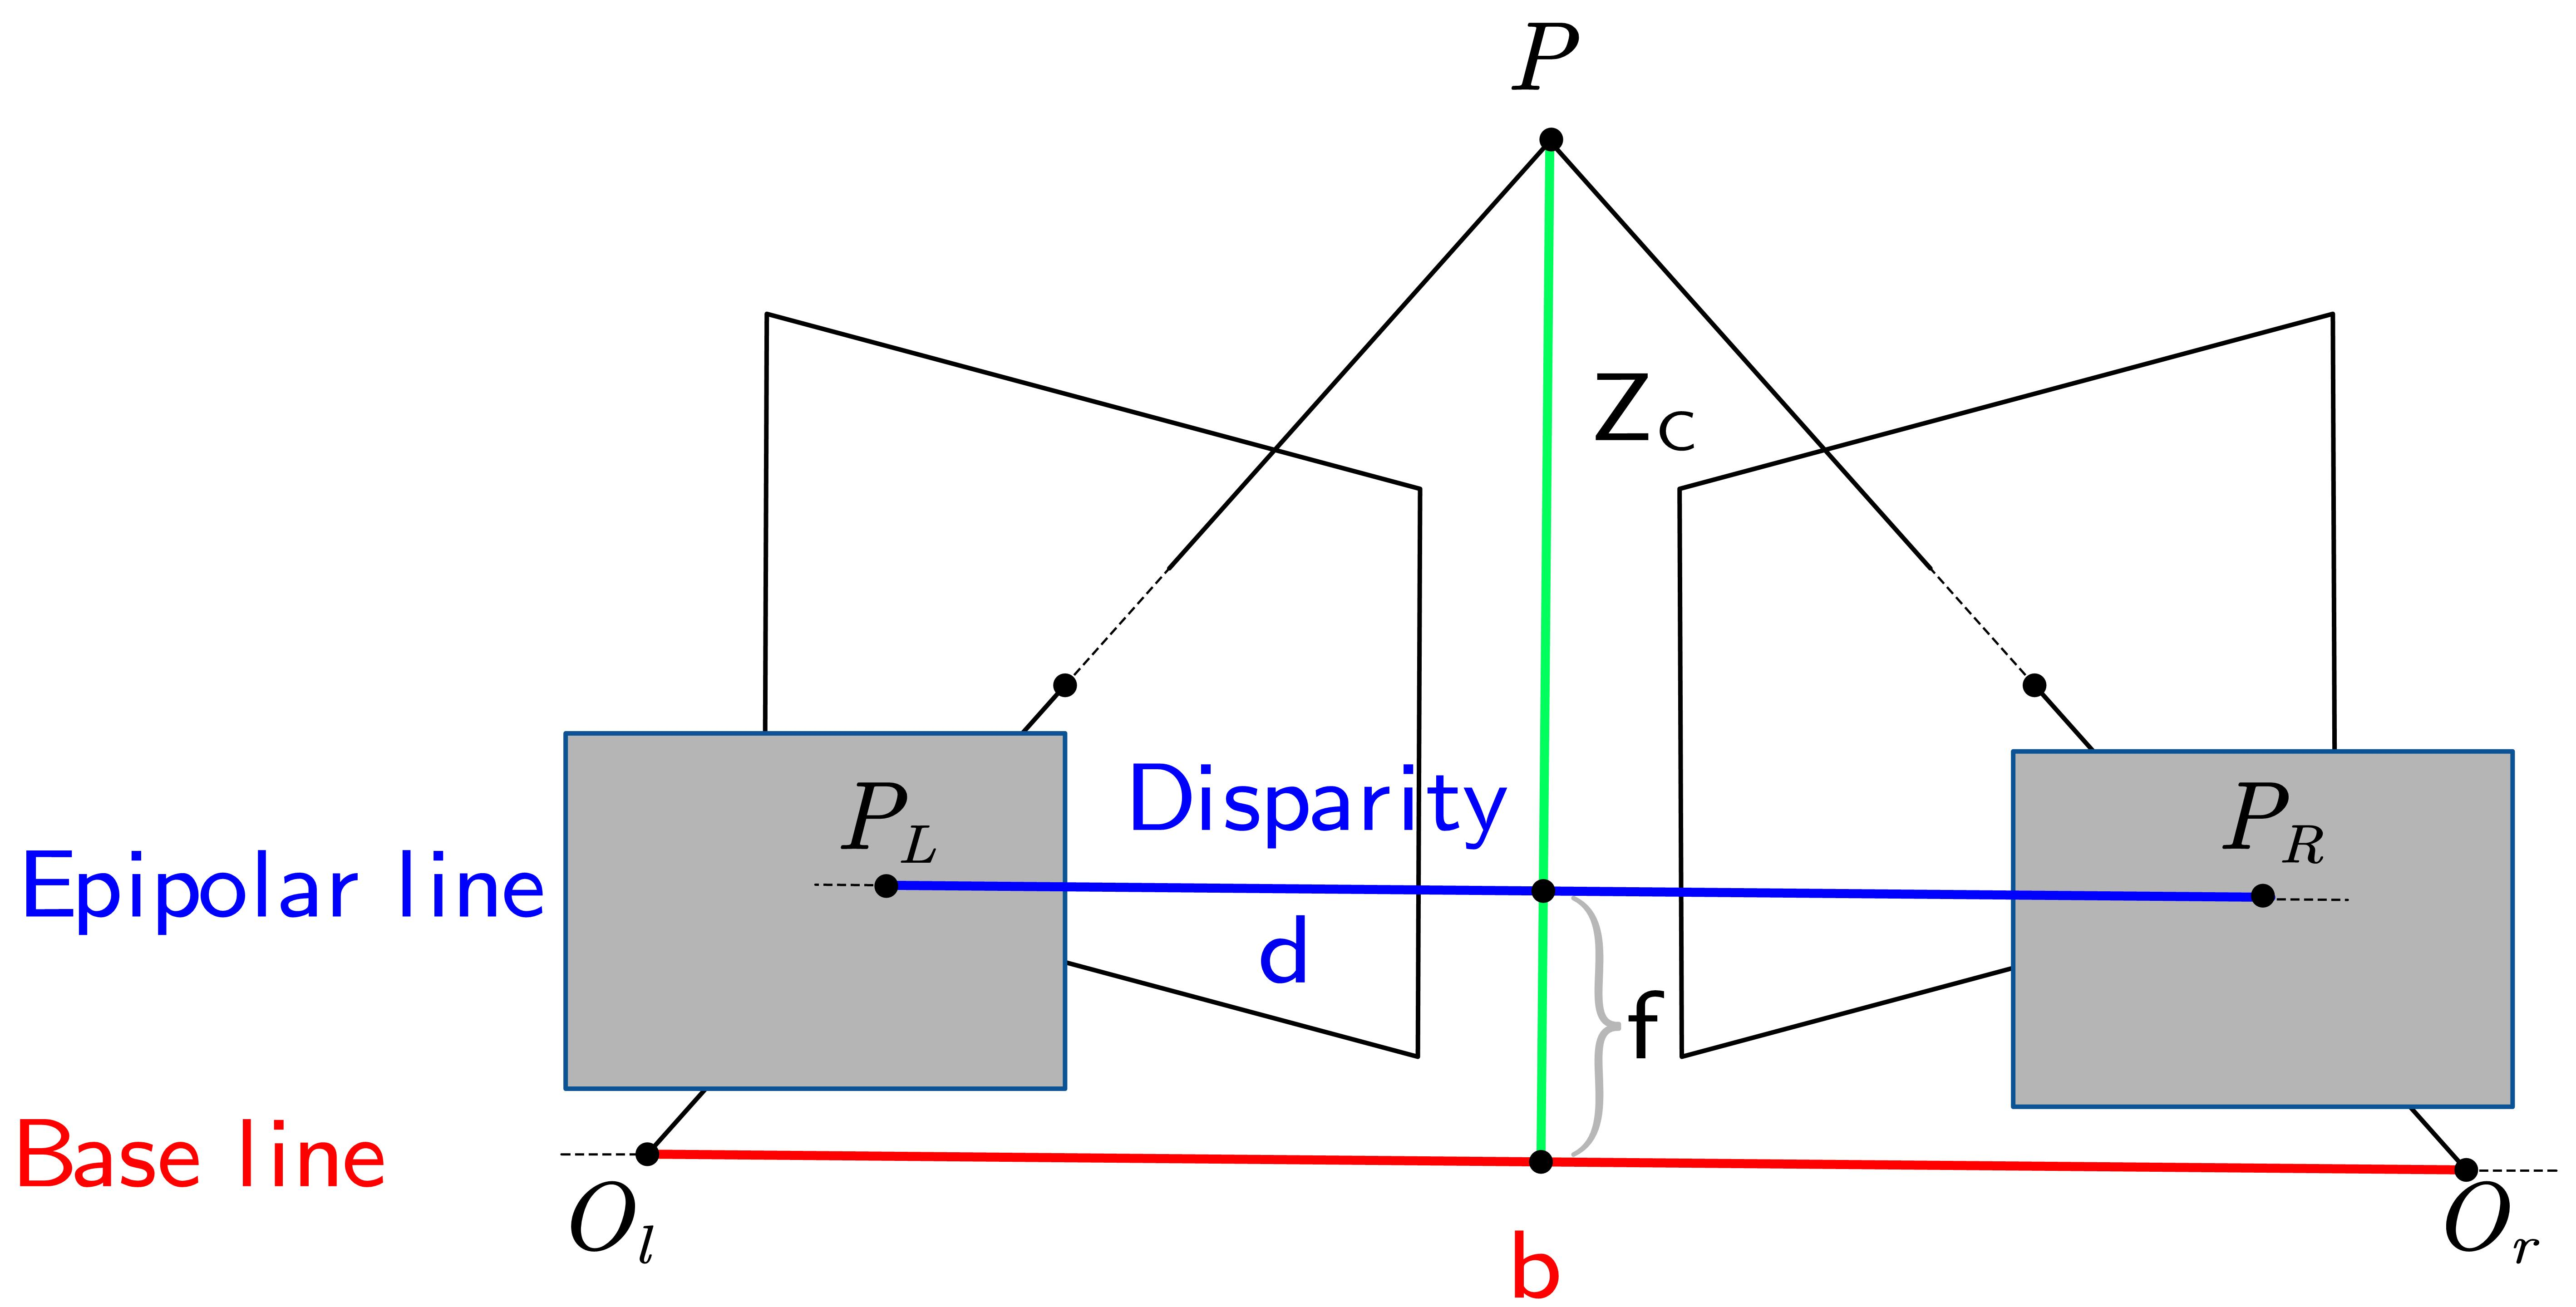
\includegraphics[scale=0.6]{双目相机-极线校正1}
		\end{center}
		\end{figure}
		\begin{itemize}
			\item 视差(Disparity):$d$
			\item 深度:$Z_C$
		\end{itemize}
		\end{frame}
	
		\begin{frame}
		\frametitle{三角法测距}
		\begin{center}
			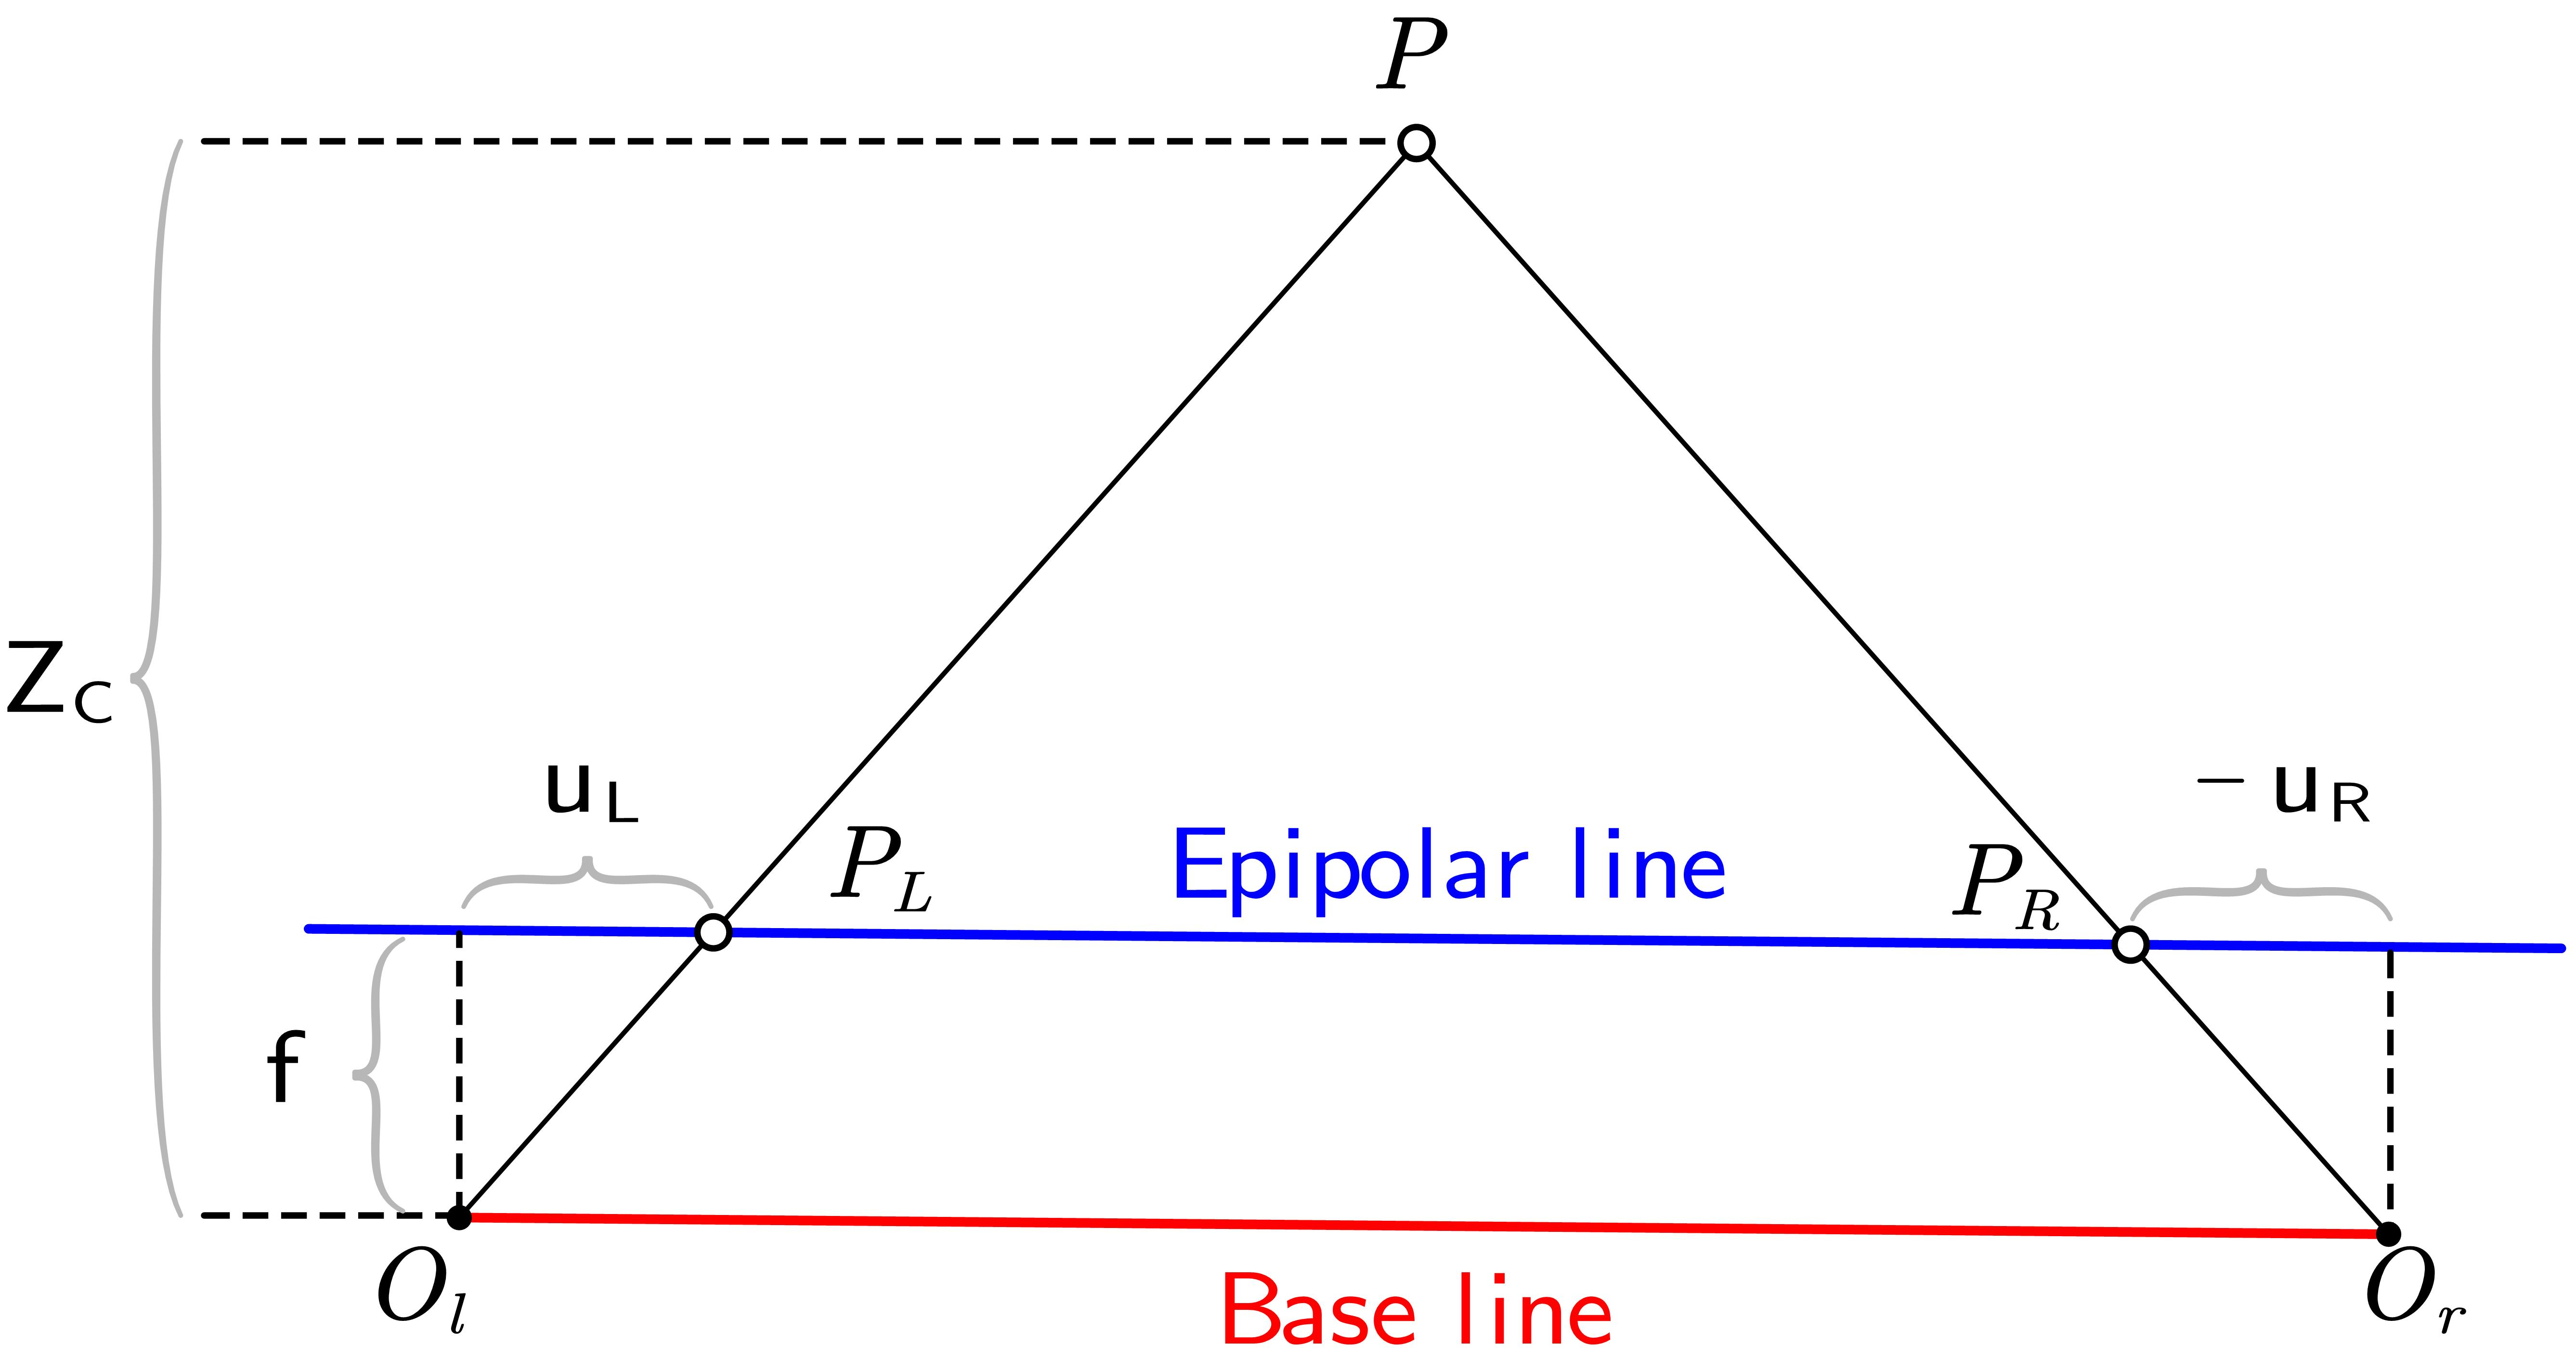
\includegraphics[scale=0.55]{双目相机-极线校正2}
		\end{center}		
		\begin{itemize}
			\item 根据相似关系:
			\begin{small}
			\begin{equation}
			\begin{aligned}
				\frac{Z_C-f}{Z_C}=\frac{b-u_L+u_R}{b}		
			\end{aligned}	
			\end{equation}
			\end{small}
			\item 整理得:
			\begin{small}	
			\begin{equation}
			\begin{aligned}
				Z_C=f\cdot \frac{b}{d},    d=u_L-u_R
			\end{aligned}	
			\end{equation}
			\end{small}
		\end{itemize}
		\end{frame}


	
	\subsection{机器人手眼标定实现物品抓取}

	\begin{frame}
	\frametitle{手眼标定}
	
	\begin{itemize}
		\item Eye-in-hand(眼在手上)
		
		相机安装在机械臂末端执行器位置,标定板不动,随着机械臂的移动,实现了相机从不同角度拍摄图像
		\item Eye-to-hand(眼在手外)
		
		相机固定不动,标定板固定在机械臂末端执行器位置,让标定板出现在相机视野中,随着机械臂的移动,实现了相机从不同角度拍摄图像

	\end{itemize}


	\begin{figure}
	\setcounter{subfigure}{0}
	\subfigure[Eye-in-hand]
	{
		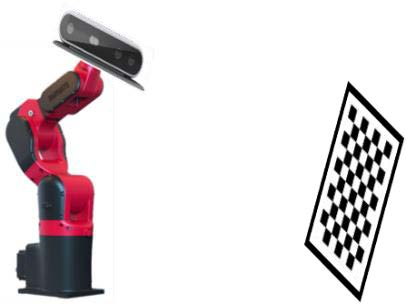
\includegraphics[scale=0.7]{Eye-in-hand}
	}
	\subfigure[Eye-to-hand]
	{
		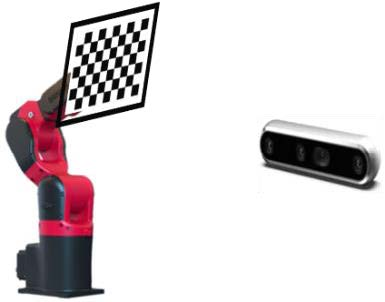
\includegraphics[scale=0.7]{Eye-to-hand}
	}
	\caption{手眼标定分类及示意图}    %大图名称
	\label{手眼标定分类}
	\end{figure}
	\end{frame}

	\section{参考文献(Reference)}
	
		\begin{frame}
			\frametitle{Reference}
			\begin{itemize}
				\item Digital Image Processing-Gonzalez
				\item Machine Vision Algorithms and Applications-Carsten Steger
				\item A flexible new technique for camera calibration-Z.Zhang
				\item 工业机器人视觉定位抓取技术的研究-杨人豪
				\item 双目视觉系统标定方法的研究-殷文茜
				\item 摄像机标定方法的研究-舒娜
			\end{itemize}
		\end{frame}
	
\end{document}